%%% Setup
%%% Dokumentenklasse Artikel
%%% 12pt
%%% A4
%%% Titelseite
%%% Nummerierung ohne endende Punkte zB. 1. ; 1.1.
%%% einseitig
\documentclass[fontsize=12pt,paper=a4,titlepage,numbers=noenddot,twoside=false,bibliography=totocnumbered,toc=listof,hidelinks,listof=totocnumbered]{scrartcl}

%%% Schriftart, Kodierung und Sprache
\usepackage[T1]{fontenc}
\usepackage[utf8]{inputenc}
\usepackage[ngerman]{babel}

%%% Erlaube größere Wortzwischenräume.
%%% Damit werden nicht mehr so viele Wörter über den Rand geschrieben.
\setlength\emergencystretch{1em}

%%% Schriftart
%\usepackage{ae}
\usepackage{times}

%%% Space :)
\usepackage{setspace}

%%% Multirow in Tabellen (miktex only?)
\usepackage{multirow}

%%% Longtable
\usepackage{longtable}

%%% Grapfikpaket
\usepackage{graphicx}

%%% Randeinstellungen
\usepackage[left=30mm,right=30mm,bottom=25mm,top=25mm]{geometry}

%%% Blindtext
\usepackage{lipsum}

%%% Footer und Header
%% headsepline - Headerlinie
%% footsepline - Fusslinie
%% mehr unter http://get-software.net/macros/latex/contrib/koma-script/doc/scrguide.pdf
\usepackage[headsepline,footsepline,automark]{scrlayer-scrpage}

%%% Formelkram falls gebraucht
%\usepackage{amsmath}
%\usepackage{amsfonts}
%\usepackage{amssymb}

%%% Listen
\usepackage{enumerate}
\usepackage{listings}
\usepackage{enumitem}

%%% Listeneinträge sollen alle mit Bullets anfangen
%\renewcommand{\labelitemi}{$\bullet$}
%\renewcommand{\labelitemii}{$\bullet$}
%\renewcommand{\labelitemiii}{$\bullet$}
%\renewcommand{\labelitemiv}{$\bullet$}

%%% Für Programm/Code Listings
\renewcommand{\lstlistingname}{Programm}

%%% Gepunktete Linie im Inhaltsverzeichnis entfernen
\usepackage[titles]{tocloft}
\renewcommand{\cftdot}{}

%%% (Kleinere) Randnotizen
\usepackage{marginnote}
\renewcommand*{\marginfont}{\footnotesize}

%%% Farbenkram
%\usepackage{color}

%%% Gedichte
\usepackage{verse}

%%% pdf zusätzlich einbinden
\usepackage{pdfpages}
\pdfoptionpdfminorversion=7

%%% PDF Hyperlinks
\usepackage[ngerman,plainpages=false,pdfpagelabels]{hyperref}

%%% Booksmarks haben ebenfalls Nummern
\hypersetup{bookmarksnumbered}

%%% biblatex (Quellenverz)
%%% mehr unter http://biblatex.dominik-wassenhoven.de/download/DTK-2_2008-biblatex-Teil1.pdf
%%% benutze biber.exe anstelle von bibtex.exe (miktex)
\usepackage[backend=biber,maxbibnames=3,bibencoding=utf8,style=authoryear-icomp,bibstyle=numeric,pagetracker=false,isbn=false,minbibnames=3,maxbibnames=3,mincitenames=3,maxcitenames=5,urldate=long,autocite=footnote]{biblatex}
\usepackage[babel,german=quotes]{csquotes}
\setlength{\bibitemsep}{1em}

\DefineBibliographyStrings{ngerman}{andothers={et\ al\adddot}}

%%% Das Quellenverz. z.B. mit JabRef erstellt. 
\bibliography{bibliography}
\addbibresource{bibliography.bib}

\DeclareNameAlias{sortname}{last-first}
\DeclareNameAlias{default}{last-first}

\AtBeginBibliography{%
  \renewcommand*{\multinamedelim}{\addsemicolon\space}
  \renewcommand*{\finalnamedelim}{\addsemicolon\space}
}

%%% Zeilenabstand 1,5
\onehalfspacing

%%% Extra Kommandos
%% \punkte -> ...
\newcommand*{\punkte}{\dots\unkern}

%\renewcommand\listoffigures{%
    %\section{\listfigurename}% Used to be \section*{\listfigurename}
      %\@mkboth{\MakeUppercase\listfigurename}%
              %{\MakeUppercase\listfigurename}%
    %\@starttoc{lof}%
    %}

\hypersetup{
	pdftitle    = {Schüler haben's schwer, Lehrer aber auch. Außerunterrichtliche Beratungs- und Unterstützungsbedarfe von SchülerInnen im medizinischen und sozialen Bereich und daraus abgeleitete sozialpädagogische Angebote},
	pdfsubject  = {Ermittlung möglicher Problemlagen von Schülern am DRK-Bildungswerk Sachsen; zudem die Sicht der Lehrer auf diese Problematik und daraus schlussfolgernd die Konzeption möglicher Beratungs- und Unterstützungsangebote},
	pdfauthor   = {Doreen Stichel, Daniela Wobst},
	pdfkeywords = {Schulsozialarbeit, Berufsbildende Schulen, Sachsen, DRK-Bildungswerk Sachsen},
	pdfcreator  = {pdflatex},
	pdfproducer = {LaTeX with hyperref}
}

%%% Hier beginnt das Dokument
\begin{document}

\KOMAoption{headsepline}{false} 
\KOMAoption{footsepline}{false}

%%% römische nummerierung
\pagenumbering{roman}

\setcounter{secnumdepth}{5}
\setcounter{tocdepth}{5}

%%% Footer und Header clearen
\clearscrheadfoot

%%% Titelseite
\begin{titlepage}
\begin{center}
\normalsize
\scshape
Technische Universität Dresden\\
\normalsize
\upshape
Fakultät Erziehungswissenschaften\\
Institut für Berufspädagogik und Berufliche Didaktiken\\
Professur für Sozialpädagogik einschließlich ihrer Didaktik\\[2,0cm]
\end{center}

\begin{center}
\Huge
\scshape
\bfseries
Masterarbeit\\[0,5cm]
\normalsize
\mdseries
im Fach Sozialpädagogik\\
\noindent\rule{\textwidth}{1pt}\\[1cm]
\normalsize
\mdseries
\textbf{Schüler haben's schwer}\\
\textbf{Lehrer aber auch}\\[0,5cm]
\normalsize
\mdseries
Außerunterrichtliche Beratungs- und Unterstützungsbedarfe von SchülerInnen im medizinischen und sozialen Bereich\\
-\\
eine explorative Analyse unter Einbeziehung der Lehrerperspektive am DRK Bildungswerk Sachsen\\[2,0cm]
\end{center}

\begin{center}
\textbf{eingereicht von:}\\
Doreen Stichel\\
Daniela Wobst\\[1,0cm]

\textbf{Erstgutachter:}\\
Prof. Dr. rer. soc. habil. Hans Gängler\\[1,0cm]
\textbf{Zweitgutachter:} \\
Dipl. Med.-Päd. Heike Haupt\\[1,0cm]

Dresden, \today
\end{center}

\end{titlepage}

\KOMAoption{footsepline}{true} 
\ofoot{\pagemark}

\begin{flushright}
	
\includegraphics[scale=0.5]{images/TU-Logo.png}
\end{flushright}

\noindent
\textbf{Doreen Stichel}\\[0,5cm]
\begin{tabular}{lll}
geboren am: & 10.02.1984\\[0,5cm]
Anschrift: & Fetscherstrasse 7\\
& 01307 Dresden\\[0,5cm]
E-Mail: & \flq{}doreens84@aol.com\frq{}\\[0,5cm]
Studiengang: & Höheres Lehramt an berufsbildenden Schulen\\
Berufliche Fachrichtung: & Gesundheit und Pflege\\
zweites studiertes Fach: & Sozialpädagogik\\[0,5cm]
Matrikelnummer: & 3686656\\[0,5cm]
immatrikuliert am: & 01. Oktober 2010\\[2cm]
\end{tabular}

\noindent
\textbf{Daniela Wobst}\\[0,5cm]
\begin{tabular}{lll}
geboren am: & 19.06.1979\\[0,5cm]
Anschrift: & Grillparzerstrasse 28\\
& 01157 Dresden\\[0,5cm]
E-Mail: & \flq{}danielawobst@aol.com\frq{}\\[0,5cm]
Studiengang: & Höheres Lehramt an berufsbildenden Schulen\\
Berufliche Fachrichtung: & Gesundheit und Pflege\\
zweites studiertes Fach: & Sozialpädagogik\\[0,5cm]
Matrikelnummer: & 3686834\\[0,5cm]
immatrikuliert am: & 01. Oktober 2010
\end{tabular}

\include{danksagung}


\begin{center}
	\textbf{Schüler haben\grq s schwer ...\footcite{prepolino2010}}
\end{center}

\begin{figure}[h]
	\centering
		
\includegraphics[width=0.4\textwidth]{images/Lasten-eines-Schuelers.jpg}\\
	\caption{Lasten eines Schülers. Prepolino 2010}
	\label{fig:Lasten-eines-Schuelers}
\end{figure}

\begin{center}
	\textbf{... Lehrer aber auch \footcite{prepolino2010}}
\end{center}

\begin{figure}[h]
	\centering
		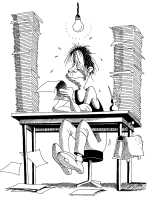
\includegraphics[width=0.4\textwidth]{images/Lasten-eines-Lehrers.jpg}\\
	\caption{Lasten eines Lehrers. Prepolino 2010}
	\label{fig:Lasten-eines-Lehrers}
\end{figure}







%%%-Hinweis
\vspace*{\fill}

\begin{flushleft}
\textbf{(1) Hinweis zur geschlechtlichen Benennung}
\end{flushleft}
Die unzureichende Bezeichnung weiblicher und männlicher Personen in dieser Arbeit bringt die verfassungsrechtlich gebotene Gleichstellung von Mann und Frau sprachlich nicht angemessen zum Ausdruck. Auf die Verwendung von Doppelformen oder andere Kennzeichnungen für weibliche und männliche Personen wird jedoch verzichtet, um die Lesbarkeit und Übersichtlichkeit zu wahren. Mit allen im Text verwendeten Personenbezeichnungen sind stets beide Geschlechter gemeint.

\begin{flushleft}
\textbf{(2) Hinweis zur beiliegenden CD}
\end{flushleft}
Die beiliegende CD enthält sowohl die PDF-Version dieses Dokumentes als auch die vollständigen Transkripte und Audiodateien der Interviews, welche für die Erarbeitung der Inhalte herangezogen wurden.

\begin{flushleft}
\textbf{(3) Hinweis zur Dokumenterstellung (\LaTeX\ und GitHub)}
\end{flushleft}
Die vorliegende Masterarbeit wurde mit \LaTeX\ erstellt. Zur Versionierung und zum Zweck der Datensicherung wurde der Quellcode des Dokumentes bei GitHub hochgeladen und liegt dort einsehbar unter folgender Adresse vor:\\
\url{https://github.com/virtualdreams/ma-schulsozialarbeit}

%%% Inhaltsverzeichnis
%%%Inhaltsverzeichnis
\pdfbookmark[1]{Inhaltsverzeichnis}{toc}
\tableofcontents


\noindent
\textbf{Zuordnung der Kapitel}\\[0,5cm]
Gemäß §21 Absatz 5 der Prüfungsordnung für den konsekutiven Master-Studiengang Höheres Lehramt an berufsbildenden Schulen kann die Masterarbeit auch in Form einer Gruppenarbeit erfolgen, solange der zu bewertende Einzelbeitrag des Studierenden kenntlich gemacht wird \footcite[vgl.][14]{TUDresden2010}.\\
Dieser Anforderung wird mittels folgender Kennzeichnung entsprochen.\\

\noindent
Doreen Stichel: S\\
Daniela Wobst: W\\

\begin{description}[nosep]
	\item[Kapitel 1:] S/W
	\item[Kapitel 2:] W
	\item[Kapitel 3:] W
	\item[Kapitel 4:] W
	\item[Kapitel 5:] S
	\item[Kapitel 6:] S
	\item[Kapitel 7:] S
	\item[Kapitel 8:] S
	\item[Kapitel 9:] W
	\item[Kapitel 10:] S/W	
\end{description}



\KOMAoption{headsepline}{true} 
%\KOMAoption{footsepline}{true} 

%%% Seitenzahl ab hier immer rechts
%\ofoot{\pagemark}
\ohead{Masterarbeit}
\ihead{\headmark}
\pagestyle{scrheadings}

%%% arabische Nummerierung
\pagenumbering{arabic}

%%% Inhalte
\section{Einleitung}
\label{sec:Einleitung}

\section{Allgemeine theoretische Grundlagen zur Schulsozialarbeit}
\label{sec:AllgemeineTheoretischeGrundlagenZurSchulsozialarbeit}

\subsection{Annäherung an eine Definition}
\label{sec:AnnäherungAnEineDefinition}

Bei der Sichtung der aktuellen Literatur zur Thematik Schulsozialarbeit wird vergleichsweise schnell deutlich, dass eine klare Definition sich durchaus als schwierig bzw. unmöglich darstellt. Nahezu alle relevanten und im weiteren Fortgang der Arbeit zitierten Autoren, stellen dies in ihren Ausführungen fest. Für ein einheitliches und unumstrittenes Begriffsverständnis scheint das Arbeitsfeld, welches zwar recht intensiv beforscht worden ist, zu heterogen und inhaltlich immer noch zu unklar \footcite[vgl.][7]{Speck2010}. Bereits bei der reinen Bezeichnung zeigen sich große Unterschiede, da einige Autoren für den Begriff der "`Sozialen Arbeit an Schulen"', andere jedoch für "`Schulsozialarbeit"' plädieren und gleichzeitig auch noch zahlreiche weitere Wortschöpfungen wie zum Beispiel "`schulbegleitende Sozialarbeit"', "`Jugendsozialarbeit an Schulen"', "`schulalltagsorientierte Sozialpädagogik"' oder "`Schoolwork"' verwendet und mit inhaltlichen Differenzierungen versehen werden \footcites[vgl.][14]{Spies2011}[vgl.][17f]{Stuewe2015}. Diese teilweise verwirrende Vielfalt lässt sich vermutlich mit unterschiedlichen theoretischen Ansätzen und praktischen Anforderungen erklären. Zur Begründung der begrifflichen Fülle wird, insbesondere von Speck \footcite[vgl.][23]{Speck2007} angeführt, dass grundsätzlich die föderale Struktur der Bundesrepublik und die Förderpolitik der einzelnen Bundesländer zu zahlreichen synonym verwendeten Begrifflichkeiten führt. Eine gewisse Vorbelastung der Schulsozialarbeit, die stärkere Betonung des Jugendhilfecharakters, die angestrebte Verknüpfung präventiver und intervenierender Angebote sowie die Vermeidung einer einseitigen und etikettierenden Zielgruppenfokussierung sind zusätzliche Gründe, welche zahlreiche Wortschöpfungen in der fachlichen Diskussion hervorbringen \footcite[vgl.][23]{Speck2007}. Dabei merkt Karsten Speck kritisch an, dass verschiedenste eingeführte Bezeichnungen selbst von den Autoren diverser Fachpublikationen nicht konsequent eingehalten werden, klare Aussagen zu Zielen und inhaltlichen Schwerpunktsetzungen oftmals fehlen und "`[a]ngenommen werden kann, dass durch die Begriffsvielfalt [\punkte] ein fachlicher Austausch, die notwendige Konzeptdiskussion und Profilschärfung sowie die Transparenz und Durchsetzung des Arbeitsfeldes in der Fachöffentlichkeit deutlich erschwert sind."' \footcite[24]{Speck2007}. Vor dem Hintergrund der genannten Begründungen und in Anlehnung an Speck, als Autor der meisten relevanten Fachpublikationen im Arbeitsfeld, soll daher in den nachfolgenden Ausführungen der Begriff "`Schulsozialarbeit"' verwendet werden, den er 2006 wie folgt definiert:

\begin{quotation}
\noindent
"`Unter Schulsozialarbeit wird im Folgenden ein Angebot der Jugendhilfe verstanden, bei dem sozialpädagogische Fachkräfte kontinuierlich am Ort Schule tätig sind und mit Lehrkräften auf einer verbindlich vereinbarten und gleichberechtigten Basis zusammenarbeiten, um junge Menschen in ihrer individuellen, sozialen, schulischen und beruflichen Entwicklung zu fördern, dazu beizutragen, Bildungsbenachteiligungen zu vermeiden und abzubauen, Erziehungsberechtigte und LehrerInnen bei der Erziehung und dem erzieherischen Kinder- und Jugendschutz zu beraten und zu unterstützen sowie zu einer schülerfreundlichen Umwelt beizutragen. Zu den sozialpädagogischen Angeboten und Hilfen der Schulsozialarbeit gehören insbesondere die Beratung und Begleitung von einzelnen SchülerInnen, die sozialpädagogische Gruppenarbeit, die Zusammenarbeit und Beratung der LehrerInnen und Erziehungsberechtigten, offene Gesprächs-, Kontakt- und Freizeitangebote, die Mitwirkung in Unterrichtsprojekten und in schulischen Gremien sowie die Kooperation und Vernetzung mit dem Gemeinwesen \footcite[28]{Speck2007}."'
\end{quotation}

\noindent
Auf diese umfangreiche Definition, die zugleich bereits einige Zielstellungen und Aufgabenschwerpunkte beinhaltet und die Schulsozialarbeit sehr breit und insbesondere als Kooperation von schulischen und sozialpädagogischen Fachkräften interpretiert, soll an diversen Stellen in dieser Arbeit nochmals zurückgegriffen und an sie angeknüpft werden. 

Eine weitere und deutlich neuere Begriffsbestimmung liefert Pötter im Jahr 2014, wobei die Kooperation verschiedener Professionen und die engere Verzahnung von außerschulischem und schulischem Leben von Kindern und Jugendlichen in den Fokus genommen werden:

\begin{quotation}
\noindent
"`Schulsozialarbeit ist das Ergebnis von Kooperationen zwischen den verschiedenen Akteuren des Systems Schule -- insbesondere zwischen den sozialpädagogischen und den schulpädagogischen Fachkräften -- mit dem Ziel, "`Anschlussfähigkeit"' zwischen den Funktionssystemen -- insbesondere dem Erziehungs- und dem Bildungssystem -- und den Lebenswelten der Kinder und Jugendlichen sicherzustellen und zu unterstützen."'\footcite[23]{Poetter2014}
\end{quotation}

\noindent
Möglicherweise liegt dieser Definition ein ganzheitlicheres Verständnis, also die weniger strenge Trennung von Schule und "`Nichtschule"' im Sinne der Lebensweltorientierung zugrunde. Dies könnte sich insbesondere bei der Betrachtung persönlicher, außerschulischer Problemlagen von Kindern und Jugendlichen und deren Einfluss auf den schulischen Bereich als durchaus sinnvoll erweisen. Daher und aufgrund ihrer Aktualität wird diese Interpretation in die theoretischen Ausführungen aufgenommen.
 
Abschließend zu diesem Teil soll noch eine letzte Begriffsbestimmung ergänzt werden, welche aufgrund des direkten Bezuges zum Bundesland Sachsen interessant für die weiteren Ausführungen erscheint. In der Handreichung des Landesjugendamtes "`Schulsozialarbeit im Freistaat Sachsen"' aus dem Jahr 2008 wird folgende ausführliche Definition zur Thematik gegeben: 

\begin{quotation}
\noindent
"`Schulsozialarbeit zielt auf Begleitung der Schülerinnen und Schüler in ihrem Prozess des Erwachsenwerdens, auf Unterstützung bei einer für sie befriedigenden Lebensbewältigung sowie auf Förderung ihrer Kompetenzen zur Lösung von persönlichen und/oder sozialen Problemen. Dabei berücksichtigt Schulsozialarbeit, dass die gesellschaftliche Teilhabe über berufliche Eingliederung (Ausbildung, Arbeit) für junge Menschen von zentraler Bedeutung ist. Die berufliche Eingliederung wiederum setzt Schulerfolg, also entsprechende Schulabschlüsse, voraus. Schulsozialarbeit als Leistungsangebot der Jugendhilfe vereint die unterschiedlichen Methoden von sozialer Arbeit "`Einzelhilfe"', "`Gruppenarbeit"' sowie "`Gemeinwesenarbeit"' innerhalb eines sozialpädagogischen Gesamtkonzeptes. Dabei sind Einzelhilfe und Gruppenarbeit konstitutive Elemente des Gesamtkonzeptes.

Durch ihren niedrigschwelligen und aufsuchenden Charakter ist Schulsozialarbeit "`Prävention und Intervention vor Ort"' und hat schwerpunktmäßig die Schülerinnen und Schüler im Blick, die aufgrund sozialer Benachteiligungen und/oder individueller Beeinträchtigungen auf besondere Unterstützung angewiesen sind. Schulsozialarbeit fördert die schulische Ausbildung und die soziale Integration. Sie trägt damit ergänzend und erweiternd zur Verwirklichung des Erziehungsauftrages der Schule bei."' \footcite[10]{SMSSSL2008}
\end{quotation}

\noindent
Auffällig in dieser Definition ist insbesondere die starke Betonung der Bedeutung beruflicher Eingliederung im Sinne von Ausbildung und Arbeit, die sich in den Ausführungen anderer Autoren so nicht findet. Weiterhin bilden die Erwähnungen der Schulsozialarbeit im Sinne von Prävention und Intervention, die ausführlichen Darstellungen der Methoden sowie die Aussagen zur Zielgruppe eine Besonderheit, auf die in den weiteren Ausführungen noch einzugehen sein wird. 

Die vorgestellten Definitionen bilden, wie bereits eingangs ausgeführt, nur eine Auswahl aus einer Fülle vielfältiger begrifflicher Erläuterungen, welche sich in einigen Punkten ähneln und vielfach auch unterscheiden. Ausgewählt wurden die hier verwendeten aus unterschiedlichen Gründen. Zum einen sollten verschiedene Herangehensweisen an das Arbeitsfeld von mehreren Autoren vorgestellt werden. Zum anderen erschien es wichtig, dass Karsten Speck als Verfasser zahlreicher, viel zitierter und grundlegender Publikationen zum Thema Schulsozialarbeit vertreten ist. Die Definition von Pötter aus dem Jahr 2014 soll aufgrund ihrer Aktualität nicht außen vor gelassen werden und die des Sächsischen Staatsministeriums für Soziales repräsentiert die ministeriale Grundauffassung zur Schulsozialarbeit im Bundesland Sachsen. Da die von den Verfasserinnen dieser Arbeit selbst durchgeführten Untersuchungen sich auf eine berufliche Schule in Sachsen fokussieren, muss diese theoretische Grundlage unbedingt mit berücksichtigt werden. 

\subsection{Rechtliche Grundlagen}
\label{sec:RechtlicheGrundlagen}

Aktuelle und prägnant-zusammenfassende Aussagen zu den Rechtsgrundlagen von Schulsozialarbeit bieten die Autoren Stüwe, Ermel und Haupt in ihrer Publikation von 2015 \footcite[24ff]{Stuewe2015}, aus der die Meisten der folgenden Aussagen entnommen sind. Zunächst muss festgehalten werden, dass derzeit keine verbindliche und bundeseinheitliche gesetzliche Regelung existiert. Daraus entstehen erhebliche länderspezifische Unterschiede in der Umsetzung, Wirksamkeit und Finanzierung von Schulsozialarbeit. Unter anderem ist es diese Heterogenität, welche bis in die differenzierten Bezeichnungen für Schulsozialarbeit hineinwirkt, die grundlegende Probleme im Arbeitsfeld bedingt (vgl. Punkt \ref{sec:AnnäherungAnEineDefinition} in Anlehnung an \cite[23]{Speck2007}).

Gesetzliche und bundesrechtliche Einflussfaktoren auf die Schulsozialarbeit sind der originäre Bildungs- und Erziehungsauftrag der Schule (Artikel 7 des Grundgesetzes in Verbindung mit dem Schulgesetz), der Erziehungs- und Bildungsauftrag der Eltern (Artikel 6 des Grundgesetzes) sowie das Wächteramt des Staates (Artikel 6 des Grundgesetzes), ausgeführt durch Schule und Jugendamt \footcite[vgl.][25]{Stuewe2015}.

\begin{quotation}
\noindent
"`Es gibt keine eigene Gesetzesnorm für Schulsozialarbeit, sondern dieses Aufgabengebiet wird abgeleitet aus dem SGB VIII (Sozialgesetzbuch) auf Bundesebene und den schulrechtlichen Regelungen in der Autorität der jeweiligen Bundesländer. Vor diesem Hintergrund müssen die rechtlichen Grundlagen der Kinder- und Jugendhilfe und die schulrechtliche Situation des jeweiligen Bundeslandes berücksichtigt werden und es gilt zu prüfen, inwieweit im entsprechenden Schulgesetz des Bundeslandes eine Kooperation von Schule mit der Kinder- und Jugendhilfe verankert ist."' \footcite[vgl.][25]{Stuewe2015}
\end{quotation}

\noindent
Ergänzend zu dieser Aussage ist zu erwähnen, dass in den Fachgremien der einzelnen Bundesländer sowie in der Expertenschaft allgemein eine große Uneinigkeit bezüglich der Ableitung der rechtlichen Auftragsgrundlage aus dem SBG VIII/KJHG (Kinder- und Jugendhilfegesetz) vorherrscht. Entscheidend in dieser Frage sind die §§ 11 (Jugendarbeit) und 13 (Jugendsozialarbeit) des SGB VIII/KJHG. 

\begin{quotation}
\noindent
"`Hinter dieser rechtlichen Diskussion steht letztlich die viel entscheidendere Frage, ob die Schulsozialarbeit ausschließlich einen intervenierenden Auftrag (§ 13) oder ausdrücklich auch einen primären Präventionsauftrag (§ 11) hat. Aus der Beantwortung dieser Frage, ergeben sich beachtliche Konsequenzen für die Ziele, Zielgruppen und Angebote der anvisierten Schulsozialarbeit."' \footcite[22]{Speck2006}
\end{quotation}

\noindent
Zur Verdeutlichung der oben ausgeführten Schwerpunkte wird nachfolgend das Schulgesetz des Freistaates Sachsen (SchulG) exemplarisch bezüglich der genannten Aussagen geprüft. Dabei ist festzustellen, dass sich konkrete Regelungen zur Schulsozialarbeit im Schulgesetz nicht finden. Eine kurze Erwähnung findet diese, unter Verwendung verschiedener Bezeichnungen, lediglich in folgenden Abschnitten: 
\begin{itemize}
	\item § 8 Berufsschule, Absatz 4: Die Berufsschule kann für Jugendliche, die zu Beginn der Berufsschulpflicht ein Berufsausbildungsverhältnis nicht nachweisen, als einjährige Vollzeitschule (Berufsvorbereitungsjahr) geführt werden. Jugendliche im Berufsvorbereitungsjahr sind \textbf{sozialpädagogisch zu betreuen}. \footcite[7]{SMKSK2010}
	\item § 16 Ganztagsangebote, Absatz 2: Zulässige Formen von Ganztagsangeboten sind insbesondere Schulklubs, Arbeitsgemeinschaften, zusätzlicher Förderunterricht oder \textbf{Angebote der Schuljugendarbeit}. \footcite[9]{SMKSK2010}
	\item § 17 Bildungsberatung, Absatz 2: Zur Unterstützung der Erziehung und Hilfe bei der Lebensbewältigung der Schüler durch die Eltern und Lehrer wird eine schulpsychologische Beratung ermöglicht, die schulartübergreifend durch Schulpsychologen mit Hilfe von Beratungslehrern erfolgt und die \textbf{Schulsozialarbeit} einbezieht. \footcite[9]{SMKSK2010}
	\item § 35b Zusammenarbeit: Die Schulen arbeiten mit den \textbf{Trägern der öffentlichen und der freien Jugendhilfe} und mit außerschulischen Einrichtungen, insbesondere Betrieben, Vereinen, Kirchen, Kunst- und Musikschulen und Einrichtungen der Weiterbildung, sowie mit Partnerschulen im In- und Ausland zusammen. \footcite[17]{SMKSK2010}
\end{itemize}

\noindent
Weitere Ausführungen zur Regelung der Schulsozialarbeit in Sachsen finden sich in diversen Verwaltungsvorschriften und Erlassen, beispielsweise in der Förderzuständigkeitsverordnung des Sächsischen Ministeriums für Kultus (SMKFördZuVO) im § 4 Förderprogramme zur Erfüllung besonderer schulischer Aufgaben, Abschnitt 2 (Maßnahmen zur sozialpädagogischen Betreuung Jugendlicher im Berufsvorbereitungsjahr) und Abschnitt 3 (Maßnahmen der Schuljugendarbeit) \footcite[1f]{SMKSK2015b}. Eine spezielle Verwaltungsvorschrift, ein Erlass oder eine Verordnung zur Schulsozialarbeit existiert derzeit nicht.

Stüwe, Ermel und Haupt weisen in ihren Ausführungen darauf hin, dass die rechtliche Verankerung und prinzipielle Regelung von Schulsozialarbeit in Deutschland derzeit als unzureichend bewertet werden kann \footcite[30]{Stuewe2015}. 

\begin{quotation}
\noindent
"`Anzustreben ist daher eine verbindlichere Erwähnung bzw. Verankerung [\punkte] sowohl im SGB VIII, als auch in den entsprechenden Schulgesetzen, da dies zu einer Verstetigung und Professionalisierung dieses Handlungsfeldes beitragen könnte."' \footcite[30]{Stuewe2015}
\end{quotation}

\subsection{Träger der Schulsozialarbeit}
\label{sec:TrägerDerSchulsozialarbeit}

Aus den im letzten Abschnitt aufgeführten rechtlichen Grundlagen der Schulsozialarbeit ergeben sich keinesfalls automatisch zuständige "`Ausführende"' im Sinne von festgelegten Behörden oder Institutionen. Auch hier ist innerhalb Deutschlands und innerhalb der Bundesländer eine Vielzahl von unterschiedlichen Modellen und Konstellationen vorzufinden. 

\begin{quotation}
\noindent
"`Für die Schulsozialarbeit ist es nicht unerheblich, unter welchen Trägerkonstellationen sie zukünftig stattfindet. Mit der Wahl eines Trägers werden in der Regel sowohl die Dienst- und Fachaufsicht bestimmt als auch konzeptionelle und inhaltliche Prämissen gesetzt."' \footcite{BIVSD2013}
\end{quotation}

\noindent
Die in der Praxis hauptsächlich vorkommenden Trägerkonstrukte lassen sich in drei Schwerpunkte einteilen, welche im Folgenden stichpunktartig kurz vorgestellt werden sollen (alle Informationen entstammen der Bundesweiten Informations- und Vernetzungsseite zur Schulsozialarbeit in Deutschland \footcite{BIVSD2013}:\\

\noindent
\textbf{Örtlicher Schulträger (Ministerium oder Schulamt) bzw. Einzelschule}
\begin{itemize}
	\item Anstellung des Schulsozialarbeiters beim örtlichen Schulträger bzw. der Einzelschule 
	\item Schulsozialarbeiter unterliegt der Schulhierarchie
	\item Dienstaufsicht und zumeist auch Fachaufsicht liegt bei der Schule bzw. dem Schulträger
	\item Vorteile: enge Einbindung der Schulsozialarbeit in den Arbeits- und Kooperationszusammenhang der Schule, keine Barrieren und Vorbehalte gegen einen engen Einbezug von Schulsozialarbeitern in unterrichtliche und außerunterrichtliche Arbeitszusammenhänge und Entscheidungsgremien
	\item Nachteile: mögliche Vereinnahmung und Unterordnung der Schulsozialarbeiter unter schulische Zwecke, Gefahr der Überladung mit schulischen Anforderungen (Feuerwehrfunktion, Vertretung bei Unterrichtsausfall und Betreuungsdienste), sozialpädagogische Ziele, Aufgaben und Arbeitsprinzipien zweitrangig
	\item Hinweis: Fachaufsicht aus der schulischen Hierarchie herauslösen, an einen Träger der Jugendhilfe (z. B. das Jugendamt) delegieren
\end{itemize}

\noindent
\textbf{Örtliches Jugendamt}
\begin{itemize}
	\item Schulsozialarbeiter ist Angestellter des Jugendamtes
	\item örtliches Jugendamt als Dienst- und Fachaufsicht 
	\item Vorteile: enge Verbindung von Schule und Jugendhilfe, gemeinsame Arbeitsgrundlage für Schulsozialarbeiter verschiedener Schulen ist gegeben 
	\item Nachteile: Lehrer fühlen sich durch die Tätigkeit der Jugendhilfe kontrolliert bzw. indirekt kritisiert 
\end{itemize}

\noindent
\textbf{Freier Träger der Jugendhilfe}
\begin{itemize}
	\item Freier Träger kann ein etablierter Wohlfahrtsverband (Arbeiterwohlfahrt, Deutscher Caritasverband, Deutsches Rotes Kreuz, Diakonisches Werk, Deutscher Paritätischer Wohlfahrtsverband, Zentralwohlfahrtsstelle der Juden), ein Jugendverband (z. B. Evangelische Jugend Deutschlands, Feuerwehrjugend, Sportjugend, Deutscher Pfandfinderbund, Gewerkschaftsbund) oder ein kleiner, örtlicher bzw. sogar für die Schulsozialarbeit initiierter Träger (z. B. eingetragener Verein, Elterninitiative, Schulverein etc.) sein.
	\item Anstellung des Schulsozialarbeiters beim freien Träger
	\item Vorteile: fachliche Erfahrungen und Kompetenzen bei großen wohlfahrts- und jugendverbandlichen Trägern (auch in verwandten Arbeitsfeldern), bei Konflikten mit der Institution Schule großer (fach-)politischen Einfluss, besonderes freiwilliges Engagement kleiner Träger, gute Beziehungen zum örtlichen Schulumfeld, größere Flexibilität
	\item Nachteile: strukturelle Schwäche kleinerer Träger in finanzieller, personeller und organisatorischer Hinsicht, Probleme bei der langfristigen Absicherung und Stabilität der Schulsozialarbeit 
\end{itemize}

\noindent
Zusätzlich zu den genannten Trägerkonstrukten sind auch Mischformen, beispielsweise eine Trägerschaft durch sowohl einen öffentlichen oder freien Jugendhilfeträger in Kombination mit dem Schulamt möglich \footcite[vgl.][63]{Spies2011}. Grundsätzlich lässt sich laut Speck \footcite{BIVSD2013} keine Trägerkonstellation eindeutig favorisieren.

\begin{quotation}
\noindent
"`Die Wahl eines möglichen Trägers von Schulsozialarbeit sollte daher in erster Linie aufgrund seiner fachlichen Kompetenz in Bezug auf die Schulsozialarbeit erfolgen. Zur Trägerkompetenz gehören unter anderem die Entwicklung eines sozialpädagogisch fundierten Konzeptes, ein offensives und vorurteilsfreies Zugehen auf die Schulen, die Implementierung von fachlichen Qualitätsstandards in den Schulen, die fachliche Anleitung, Begleitung, Fortbildung und "`Rückendeckung"' für die sozialpädagogischen Fachkräfte in Schulen, die Vernetzung der Fachkräfte mit anderen SchulsozialarbeiterInnen sowie die Unterstützung der Evaluation und Qualitätsentwicklung der Schulsozialarbeit."' \footcite{BIVSD2013}
\end{quotation}

\noindent
Zur Sicherstellung dieser vielfältigen Anforderungen muss der jeweilige Träger über personelle, zeitliche und fachliche Ressourcen verfügen \footcite[vgl.]{BIVSD2013}. Weiterhin weißt Speck auf die Bedeutung von Kooperationen bei der Initiierung von Schulsozialarbeit zwischen dem Träger, der Schule, dem Schulträger und dem Jugendamt hin, welche er als überaus sinnvoll erachtet. Spies und Pötter empfehlen in Anlehnung an zahlreiche Autoren sozialpädagogischer Veröffentlichungen, dass die Schulsozialarbeit bestenfalls bei einem Jugendhilfeträger anzusiedeln ist \footcite[64]{Spies2011}. 

\begin{quotation}
\noindent
"`Ein Hauptargument dafür ist, dass die Dienst- und Fachaufsicht für die SozialarbeiterInnen bei einem Träger liegen sollte, der das fachliche -- also sozialpädagogische -- Know-How besitzt und außerhalb der stark hierarchisch organisierten Schulstruktur steht."' \footcite[64]{Spies2011}
\end{quotation}

\noindent
Dennoch werden auch Projekte mit einer kooperativen Trägerschaft von Jugendhilfe und Schule als sinnvoll erachtet, da oftmals eine bessere Zusammenarbeit mit der Institution Schule gewährleistet wird, von Beginn an größere Ressourcen beider Partner in die Kooperation einfließen und die Schule eine größere formale Verantwortung mit verstärktem Interesse am Erfolg des Projektes übernimmt \footcite[vgl.][64]{Spies2011}.

Inwieweit die genannten und beschriebenen Trägerkonstrukte für Projekte der Schulsozialarbeit an berufsbildenden Schulen eine Bedeutung haben, kann aus der Fachliteratur nicht herausgearbeitet werden. Es kann an dieser Stelle nur davon ausgegangen werden, dass die genannten Vor- und Nachteile sowie die Nützlichkeit von Kooperationen für diese Schulform ebenso zutreffen wie auf alle anderen. 

\subsection{Zielgruppen}
\label{sec:Zielgruppen}

Als Zielgruppen der Schulsozialarbeit im Allgemeinen können die Adressaten der Jugendhilfe verstanden werden, zu denen alle Kinder und Jugendlichen, Eltern und Lehrkräfte gehören \footcite[vgl.][31]{Speck2007}. Auch hierüber herrscht jedoch in der Fachwelt keinesfalls Einigkeit, kontrovers diskutiert wird von einigen Autoren die Zugehörigkeit der Lehrkräfte zur Zielgruppe. Vielmehr verorten einige diese wiederum unter dem Begriff Kooperationspartner \footcite[vgl.][50]{Spies2011}. 

\begin{quotation}
\noindent
"`Wie es unter Kooperationspartnern üblich ist, kann und sollte man sich gegenseitig informieren, beraten und unterstützen. Eventuell kann man in dem einen oder anderen Fall auch zwischen Schülern und Lehrern oder Eltern und Lehrern vermitteln [\punkte]."' \footcite[vgl.][50]{Spies2011}
\end{quotation}

\noindent
Würde man jedoch die Beratung und Unterstützung von Lehrkräften als immanenten Tätigkeitsbereich der Schulsozialarbeit begreifen, könnten die Lehrenden auch wiederum als Zielgruppe verstanden werden.

Lange Zeit richteten sich die Angebote der Jugendhilfe vorwiegend an benachteiligte junge Menschen, diese Orientierung wurde jedoch durch die Neuausrichtung des Sozialgesetzbuches VIII/KJHG von 1991 eigentlich weitestgehend aufgehoben. Stattdessen betont die gültige gesetzliche Grundlage einen stark präventiven, partizipatorischen und freiwilligen Dienstleistungscharakter der Jugendhilfe. Insbesondere die Formulierungen "`junge Menschen in der sozialen Entwicklung fördern und dazu beitragen, Benachteiligungen zu vermeiden und abzubauen"' sowie "`positive Lebensbedingungen für junge Menschen und deren Familien schaffen"' unterstreichen diese Feststellungen \footcites[vgl.][30f]{Speck2007}[vgl.][46]{Spies2011}. 

Dennoch herrscht, wie im Punkt rechtliche Grundlagen bereits ausgeführt, Uneinigkeit über die Umsetzung dieser gesetzlichen Grundlage und die sich daraus ergebenden primären Zielgruppen der Schulsozialarbeit. Erstaunlicherweise fokussiert die im Abschnitt \ref{sec:AnnäherungAnEineDefinition} vorgestellte Definition von Schulsozialarbeit des Sächsischen Landesjugendamtes insbesondere auf "`[\punkte] Schülerinnen und Schüler [\punkte], die aufgrund sozialer Benachteiligungen und/oder individueller Beeinträchtigungen auf besondere Unterstützung angewiesen sind."' \footcite[10]{SMSSSL2008} Hier ergibt sich eine jedoch nur scheinbar eine sächsische Besonderheit, da ein Vergleich der jeweiligen Länderpraxen von Speck aufzeigt, dass in fast allen Bundesländern Schwerpunkte bei Jugendlichen, die am Übergang von der Schule in die Erwerbstätigkeit zu scheitern drohen und Schülern in Hauptschulbildungsgängen gesetzt werden \footcite[vgl.][19ff]{Speck2007}. Dabei konstatiert Speck auch eine besondere Verpflichtung der Schulsozialarbeit, mit ihren Angeboten benachteiligte und beeinträchtigte SchülerInnen zu erreichen und diese zu unterstützen, gleichzeitig soll sich diese jedoch keinesfalls auf diesen problem- oder defizitorientierten Ansatz beschränken \footcite[vgl.][46]{Speck2007}. 
\begin{quotation}
\noindent
"`Bei einem solchen Ansatz sind a) Defizitorientierung und Stigmatisierung der Schüler, b) eine geringe Mitwirkungsbereitschaft der Schüler sowie c) problematische konzeptionelle Beschränkungen, die dem Bild einer präventiven, lebensweltorientierten und anwaltschaftlichen Jugendhilfe widersprechen, vorprogrammiert. Zudem würden Ressourcen, Kooperationsmöglichkeiten und Wirkungspotentiale der Schulsozialarbeit ungenutzt bleiben."'\footcite[vgl.][46]{Speck2007}
\end{quotation}
 
\noindent
Weiterführende Aussagen zur Thematik formulieren Spies und Pötter, indem sie feststellen, dass "`[s]chulpflichtige Kinder und Jugendliche aller Altersstufen und unabhängig von der Schulform und der Trägerschaft der Schule [\punkte] grundsätzlich die Zielgruppe der Schulsozialarbeit sind."' \footcite[46]{Spies2011} Allerdings reichen die Projekte und Möglichkeiten der Schulsozialarbeit gar nicht aus, um überhaupt allen genannten Zielpersonen ein Angebot zu machen, was sich als durchaus problematisch erweist. Dies zwingt die im Handlungsfeld tätigen Personen letztlich dazu, ihre Adressaten einzugrenzen und erfordert Schwerpunktsetzungen, die praktisch zur Folge haben, dass doch wieder vermeintlich sozial benachteiligte und individuell beeinträchtigte Kinder und Jugendliche im Fokus der Arbeit stehen bzw. stehen müssen \footcite[vgl.][47]{Spies2011}.
 
Bezogen auf die beruflichen Schulen lässt sich festhalten, dass die dort stattfindende soziale Arbeit grundsätzlich alle Schülerinnen und Schüler ansprechen sollte, jedoch aufgrund der oben geschilderten praktischen Problemstellungen ähnlichen institutionellen Bedingungen unterworfen ist wie an allgemeinbildenden Schulen. Dabei  bilden ganz allgemein formuliert Jugendliche, sowohl mit Ausbildungsplatz als auch ohne, die Zielgruppe der berufsschulischen Sozialarbeit \footcite[vgl.][5]{ASSB2011}. Einzig Stüwe, Ermel und Haupt nehmen von allen Autoren, die sich mit theoretischen Grundlagen zur Thematik beschäftigen, in ihren Ausführungen überhaupt auf diese Schulform Bezug:

\begin{quotation}
\noindent
"`Eine besondere Rolle nimmt die Schulsozialarbeit an den berufsbildenden Schulen ein. Hier hat sie vor allem die Funktion einer Begleitung bei der Gestaltung des Übergangs in das Arbeitsleben und bei der Lösung individueller Konflikte und Defizite. Durch die einzelfallbezogenen Schwerpunktsetzungen sind somit die Zielgruppenfragen anders zu stellen."' \footcite[74]{Stuewe2015}
\end{quotation}

\noindent
Über die tatsächliche Fülle der Angebote für die genannten Zielgruppen, speziell bezogen auf den Freistaat Sachsen, wird an anderer Stelle der vorliegenden Arbeit noch ausführlich einzugehen sein. 

\subsection{Ziele}
\label{sec:Ziele}

Grundlegende Zielstellungen der Schulsozialarbeit finden sich relativ wenige in der vorhandenen Literatur, was dem geschuldet sein könnte, dass je nach definitorischem und zielgruppenbezogenem Ansatz durchaus sehr individuelle Ziele möglich sein könnten. Weiterhin spielen auch die jeweilige Schulform, das Schülerklientel, die institutionellen und finanziellen Gegebenheiten sowie die gesetzlichen Grundlagen des jeweiligen Bundeslandes bei der Betrachtung der Zielstellungen eine Rolle. 

Allgemeingültige Aussagen lassen sich primär aus den in Punkt \ref{sec:AnnäherungAnEineDefinition} benannten Definitionen herausarbeiten und sind auch dabei durchaus als heterogen zu bezeichnen. Laut Speck bestehen sie vordergründig in der Förderung junger Menschen in ihrer individuellen, sozialen, schulischen und beruflichen Entwicklung. Weiterhin soll und muss Schulsozialarbeit dazu beizutragen, Bildungsbenachteiligungen zu vermeiden und abzubauen sowie Erziehungsberechtigte und Lehrkräfte bei der Erziehung und dem erzieherischen Kinder- und Jugendschutz zu beraten und zu unterstützen sowie zu einer schülerfreundlichen Umwelt beizutragen \footcite[vgl.][28]{Speck2007}.

Folgt man hingegen der Definition von Pötter, so ist das vordergründige "`[\punkte] Ziel, Anschlussfähigkeit zwischen den Funktionssystemen -- insbesondere dem Erziehungs- und dem Bildungssystem -- und den Lebenswelten der Kinder und Jugendlichen sicherzustellen und zu unterstützen."' \footcite[23]{Poetter2014} Diese Anschlussfähigkeit definiert Pötter als wichtigen Parameter in einem jeweiligen spezifischen Kontext, "`[\punkte] der die Lebenswelten der Kinder und Jugendlichen und die gesellschaftlichen Strukturen und Anforderungen am Ort Schule miteinander verknüpft und dessen Aufgabe es ist, einerseits auf kommende Strukturen vorzubereiten und der andererseits bereits Chancen und Möglichkeiten innerhalb dieser Strukturen verteilt."' \footcite[24]{Poetter2014} Abgeleitet werden kann daraus, dass bei dieser Betrachtungsweise das Ziel der Schulsozialarbeit in der vielfältigen Nutzbarmachung von unterschiedlichen Angeboten und Chancen für alle Schüler in der derzeitigen Schulform liegt und gleichzeitig auch individuell gelingende Übergänge in weiterführende Schulformen oder in die berufliche Ausbildung sichergestellt, unterstützt und begleitet werden sollen.
 
Das Landesjugendamt des Freistaates Sachsen formuliert ganz ähnliche Zielstellungen, jedoch etwas einfacher und praktischer. 

\begin{quotation}
\noindent
"`Schulsozialarbeit zielt auf Begleitung der Schülerinnen und Schüler in ihrem Prozess des Erwachsenwerdens, auf Unterstützung bei einer für sie befriedigenden Lebensbewältigung sowie auf Förderung ihrer Kompetenzen zur Lösung von persönlichen und/oder sozialen Problemen. Dabei berücksichtigt Schulsozialarbeit, dass die gesellschaftliche Teilhabe über berufliche Eingliederung (Ausbildung, Arbeit) für junge Menschen von zentraler Bedeutung ist."' \footcite[15]{SMSSSL2008}
\end{quotation}

\noindent
Neben der Begleitung Heranwachsender stehen hier insbesondere die Kompetenzförderung bei individuellen Problemlagen und die Förderung der Anschlussfähigkeit, im Sinne der Eingliederung in Ausbildung und Berufstätigkeit, im Vordergrund. 

Spezifische Zielstellungen zur Schulsozialarbeit an berufsbildenden Schulen existieren derzeit nicht. Bezüglich der genannten Aussagen ist jedoch festzustellen, dass diese zweifelsohne auch für den berufsbildenden Bereich gelten können. Neben der Förderung und Herausbildung beruflicher Handlungskompetenzen kann in dieser Schulform immer wieder auch die Förderung persönlicher Kompetenzen und die Unterstützung von Anschlussfähigkeit in eine weiterführende Ausbildung oder eine Erwerbstätigkeit als Ziel verstanden werden. Ob insbesondere die persönliche Problemlösekompetenz und die Unterstützung der Anschlussfähigkeit als Ziele auf die Schulsozialarbeit beschränkt sind oder nicht auch Ziele der Schule und der pädagogischen Fachkräfte sein können und müssen, könnte kritisch diskutiert werden. 

\subsection{Aufgabenfelder}
\label{sec:Aufgabenfelder}

Wie bereits in den Definitionsversuchen zur Schulsozialarbeit ausgeführt, finden sich auch zu den Arbeitsbereichen und Aufgabenfeldern in der verwendeten Fachliteratur unterschiedlichste Darstellungen, Leistungsschwerpunkte und Kategorien. Insbesondere Speck weist darauf hin, dass es für die notwendige Etablierung von Schulsozialarbeit unerlässlich ist, ein klares Arbeitsprofil herauszuarbeiten, welches bestimmte Kernleistungen (gemäß dem Förderauftrag für die schulische und außerschulische Entwicklung) beinhalten sollte, die als ergänzungsoffene Pflichtaufgaben zu verstehen sind \footcite[vgl.][62]{Speck2007}. Orientiert am Konzept der lebensweltorientierten Schulsozialarbeit im Rahmen der Jugendhilfe und an den Befunden dessen wissenschaftlicher Begleitung lassen sich nach Speck folgende sechs Kernleistungen bzw. -aufgaben herauskristallisieren: 
\begin{itemize}
	\item \textbf{Beratung und Begleitung von einzelnen SchülerInnen} (z. B. Einzelfallhilfe, Beratungsgespräche, Einzelförderung, Sprechstunden)
	\item \textbf{sozialpädagogische Gruppenarbeit} (z. B. berufsorientierende Angebote, erlebnispädagogische Maßnahmen, soziales Kompetenztraining, außerunterrichtliche Projekte, offenes Förderangebot)
	\item \textbf{offene Gesprächs-, Kontakt- und Freizeitangebote} (z. B. Schülerclub, offener Treff, Freizeitangebote)
	\item \textbf{Mitwirkung an Unterrichtsprojekten und in schulischen Gremien} (z. B. Gesamtkonferenzen, Klassenkonferenzen, Schulprogrammarbeit)
	\item \textbf{Zusammenarbeit mit und Beratung der LehrerInnen und Erziehungsberechtigungen} (z. B. Beratungsgespräche, Fortbildungen, Elterngespräche, Elternabende und -besuche)
	\item \textbf{Kooperation und Vernetzung mit dem Gemeinwesen} (z. B. Jugendamt, Arbeitsverwaltung, Ämter, freie Träger der Jugendhilfe, Aufbau von Hilfestrukturen, Integration von Personen, Unternehmen und Institutionen aus dem Gemeinwesen \footcite[vgl.][63f]{Speck2007}.
\end{itemize}

\noindent
Eine hilfreiche Erweiterung der Thematik bieten Spies und Pötter, indem sie konstatieren, dass "`[s]tets Ermöglichung von Schulerfolgen, Abbau von Lernbarrieren, Sicherung verwertbarer Abschlüsse und Gewährleistung von schulischer Haltekraft die Leitgedanken sind, die hinter der schulsozialarbeiterischen Deklination jedes Arbeitsbereiches stehen"' \footcite[93]{Spies2011}. Die Autorinnen unterteilen die bereits von Speck formulierten Kernleistungen der Schulsozialarbeit dazu in drei Arbeitsbereiche, nämlich "`Bildungsbedingungen"', "`individuelle Orientierung und Hilfe"' sowie "`Förderung des sozialen Lernens"' und erweitern sie um die fachlichen Hintergründe der jeweiligen Aufgabenfelder. Dabei werden der "`sozialpädagogischen Expertise der Jugendhilfe"' die individuelle Förderung, sozialpädagogische Gruppenarbeit, offene Angebote und sozialpädagogische Einzelfallberatung, dem "`schulischen Hoheitsbereich"' das  Schulprogramm und dessen Entwicklung, gemeinsam mit der Berufsorientierung sowie der "`schulischen Zuständigkeit mit sozialpädagogischem Fach- und Methodeninput"' die Kooperation mit Eltern, schulbezogene Hilfen und Konfliktbewältigung zugeteilt. Unternommen wird der Versuch, "`die tatsächlichen Tätigkeiten in ihrer Bildungsfunktion abzubilden, ohne die dafür nötige Fachlichkeit zu eng an die sozialpädagogische Expertise zu binden."' \footcite[91]{Spies2011} Mit dieser Positionierung wird die Herangehensweise unterstrichen, die Schulsozialarbeit als ein Produkt der Kooperation verschiedener, an Schulen tätiger Disziplinen, insbesondere der Schul- und der Sozialpädagogik zu verstehen und davon ausgehend auch die Aufgabenbereiche der Schulsozialarbeit abzubilden.

\begin{quotation}
\noindent
"`Schulsozialarbeit dient der Sicherstellung und Unterstützung von Anschlussfähigkeit von Schülerinnen und Schülern mit unterschiedlichen sozialen und ethischen Hintergründen, deren Bildungsbedingungen sie verbessert, indem sie mit bildungswissenschaftlicher und sozialpädagogischer Expertise dazu beiträgt, bestehende Benachteiligungen abzubauen, die individuelle und soziale Entwicklung zu fördern und Empowerment-Strategien zu vermitteln. Sie ist als interinstitutionelle Vermittlungsinstanz im Bildungs- und Hilfesystem zu verstehen, die zur Verbesserung der Lern- und Lebensraumbedingungen von Kindern und Jugendlichen in Kontexten des Bildungssystems unter zu Hilfenahme eines breiten Handlungsspektrums von Lern- und Bildungssettings agiert."' \footcite[92]{Spies2011}
\end{quotation}

\noindent
Den genannten Aufgabenfeldern gibt es aus der Sicht der beruflichen Schule nichts hinzuzufügen. Die klassische sozialpädagogische Elternarbeit, geschlechtsspezifische Arbeit (Projektarbeit, Mädchenförderung) und offene Arbeit (insbesondere in Form von Kontakt- und Freizeitangeboten) rücken jedoch im genannten Handlungsfeld zugunsten von individueller Beratung, Begleitung und Unterstützung, sozialem Lernen und Projektarbeit eher in den Hintergrund  \footcite[vgl.][10]{LSS2004}.

\subsection{Methoden}
\label{sec:Methoden}

Nachdem verschiedene Grundlagen der Schulsozialarbeit bis hierhin erläutert wurden, soll nun im letzten dazugehörigen Abschnitte ein Überblick über die dazu zur Verfügung stehenden methodischen Möglichkeiten gegeben werden. Unter Methoden werden dabei "`[\punkte] zielgerichtete wissenschaftsgestützte und handlungserprobte Techniken verstanden, die sich im Rahmen einer Konzeption, orientiert an ethischen Prinzipien begründen lassen."' \footcite[25]{Kilb2009}. Weiterhin folgen sie definierten Prinzipien und vollziehen sich in bestimmten Arbeitsschritten. Bei jedem Arbeitsschritt werden Techniken und Instrumente berücksichtigt, die am besten geeignet sind, um die jeweiligen Ziele zu erreichen und als Einzelelemente von Methoden zu verstehen sind \footcite[vgl.][30]{Kilb2009}. Das fachliche Handeln des Schulsozialpädagogen orientiert sich dabei stets an den Zielgruppen, Zielen und Aufgabenfeldern und muss flexibel, variabel und bedarfsorientiert für den jeweiligen Schulstandort sein. Dabei erfordert die Praxis durch die bereits ausgeführte und insbesondere im Punkt \ref{sec:BedarfeFürSchulsozialarbeit}, Bedarfe für Schulsozialarbeit, noch auszuführende Vielfältigkeit ein großes Methodenrepertoire \footcite[vgl.][94]{Stuewe2015}. 

Festzustellen ist nach der Analyse mehrerer Quellen, dass keine spezifischen Methoden theoretisch ausgeführt und praktisch angewandt werden, da die Schulsozialarbeit unter dem methodischen Blickwinkel gesehen keine autonomes Arbeitsfeld ist \autocites[vgl.][94]{Stuewe2015}[vgl.][32]{Kilb2009}[vgl.][63]{Speck2007}. 
\begin{quotation}
\noindent
"`Für die Schulsozialarbeit bieten die Methoden der Sozialen Arbeit den fachlichen Hintergrund, der allerdings in den schulischen Kontext übertragen werden muss. Außerdem kann sie durchaus auf das methodische Repertoire der Schulpädagogik zurückgreifen -- sofern sie dies [\punkte] gründlich geprüft hat."' \footcite[67]{Spies2011}. 
\end{quotation}

\noindent
Das Methodenspektrum der Schulsozialarbeit ist damit äußerst vielfältig und kann in klassische direkt klientenbezogene Methoden, zu denen die Beratung und Einzelfallhilfe, die soziale Gruppen- und Projektarbeit und die inner- und außerschulische Gemeinwesenarbeit zählen, sowie indirekt klientenbezogene, wie Supervision und Selbstevaluation, gegliedert werden \footcites[vgl.][22]{Kilb2009}[vgl.][64]{Speck2007}. Die drei genannten klientenbezogenen Schwerpunkte sind als klassisches Methodentrio der Sozialen Arbeit bekannt \footcite[vgl.][95]{Stuewe2015}. 

\begin{quotation}
\noindent
"`Da professionelles methodisches Handeln weit über diese drei Methoden hinausgeht, ist jedoch eine feinere Kategorisierung notwendig. Schulsozialarbeit zieht zur Erreichung ihrer Ziele sehr unterschiedliche Methoden heran, die in der Theorie der Sozialen Arbeit in zwei mal zwei Kategorien unterteilt werden können."' (\cite[vgl.][95]{Stuewe2015} in Anlehnung an \cite[64f]{Speck2007})
\end{quotation}

\noindent
Direkt wirkende Angebote der Schulsozialarbeit mit Interventionsbezug sind dabei:
\begin{itemize}
	\item \textbf{Einzelfall- und primärgruppenbezogene Methoden} dienen einem gezielten und überprüfbaren Unterstützungsprozess zwischen Fachkraft und einem Kind bzw. Jugendlichen. Beispiele dafür sind die Einzelfallhilfe, sozialpädagogisch-klientenzen-\\
	trierte, systemische und lösungsorientierte Beratung, multiperspektivische Fallarbeit, Case-Management, Mediation, Familientherapie und Methoden der Gesprächsführung. 
	\item \textbf{Sekundärgruppen- und sozialraumbezogene Methoden} dienen ebenfalls einem gezielten und überprüfbaren Unterstützungsprozess, beziehen jedoch das soziale Netzwerk der Klienten (Eltern, Gruppenangehörige, Klasse, Lehrkräfte usw.), andere Gruppenmitglieder oder das Gemeinwesen mit ein. Zu dieser Methodengruppe gehören die Soziale Gruppenarbeit, Erlebnispädagogik, themenzentrierte Interaktion, themen- und zielgruppenspezifische Methoden (Suchtprävention, Mädchen- und Jungenarbeit), Sozialkompetenztraining, Empowerment, soziale Netzwerkarbeit und Gemeinwesenarbeit. 
\end{itemize}

\noindent
Neben diesen direkten wirkenden Angeboten gibt es weitere, indirekt wirkende Leistungen der Schulsozialarbeit, welche die Ziererreichung und die angestrebte Wirkung der Schulsozialarbeit unterstützen können bzw. Voraussetzungen für die Handlungsfähigkeit schaffen:
\begin{itemize}
	\item \textbf{Indirekte unterstützungsbezogene Methoden} dienen der Erhaltung und Verbesserung von Handlungsfähigkeit, Arbeitsstruktur und Professionalität der Schulsozialarbeiter sowie der Qualitätsentwicklung und -sicherung. Das Arbeitsfeld wird dabei systematisch evaluiert und reflektiert, beispielsweise mittels Supervision, Selbstevaluation, Fort- und Weiterbildung und Konzeptentwicklung. 
	\item \textbf{Struktur- und organisationsbezogene Methoden} haben das Ziel, strukturelle und organisatorische Voraussetzungen, Rahmenbedingungen und Grundlagen für konkrete Angebote zu schaffen und dienen der Abstimmung und Planung von Hilfestrukturen vor der eigentlichen Intervention. Beispielhaft können dafür Sozialmanagement, Jugendhilfeplanung sowie interdisziplinäre Diskussionen und Vernetzungen genannt werden (\cite[vgl.][96ff]{Stuewe2015} in Anlehnung an \cite[64f]{Speck2007}).
\end{itemize}

\noindent 
Der Einzelfallhilfe als Beispiel der einzelfall- und primärgruppenspezifischen Methoden scheint in der Praxis eine zentrale Bedeutung zuzukommen, da die "`[i]ndividuelle Begleitung von Schülerinnen und Schülern mit den Bezugspunkten "`Hilfen bei der Alltagsbewältigung"' und "`Biografie-Begleitung"' vor dem Hintergrund von Schulschwierigkeiten, Problemen im Elternhaus sowie Fragen, die den Übergang von der Schule in Ausbildung bzw. Ausbildung in Arbeit betreffen, häufig im Vordergrund der sozialpädagogischen Arbeit stehen. In jedem Fall sollte die Einzelfallhilfe sich am Prinzip "`Hilfe zur Selbsthilfe"' orientieren."' \footcite[23]{SMSSS2009} Die soziale Gruppenarbeit hingegen hat eine überwiegend erzieherische Intention und orientiert sich an den Problemen und Verhaltensmustern ihrer Zielgruppe. Durch die Gruppe in ihrem Gesamtgefüge und gruppenspezifische Aktivitäten können unter sozialpädagogischer Anleitung positive Sozialisationseffekte erzielt werden, wodurch die Gruppenarbeit das geeignete Übungsfeld für soziales Lernen im Rahmen der Schulsozialarbeit bildet \footcite[vgl.][24]{SMSSS2009}. Abschließend stellt die Gemeinwesenarbeit im Rahmen der Schulsozialarbeit eine Methode dar, die es sich zur Aufgabe macht, Lebenszusammenhänge und Probleme von jungen Menschen nicht nur individuell zu verstehen, sondern sie in einem Wirkungssystem zwischen Schule und dem jeweiligen sozialem Umfeld zu begreifen. Dabei wird angestrebt, Schule und Gemeinwesen besser zu vernetzen, um die Öffnung der Schule nach außen zu unterstützen und Kooperationen mit außerschulischen Einrichtungen und Institutionen zu fördern \footcite[vgl.][25]{SMSSS2009}. 

Die Einzelfallhilfe in verschiedenen Formen von Beratung und individueller Begleitung, sowie die soziale Gruppenarbeit und Projektarbeit scheinen methodisch insbesondere an beruflichen Schulen eine große Bedeutung zu haben \footcite[vgl.][10ff]{LSS2004} (vgl. Punkt \ref{sec:Aufgabenfelder}).

\subsection{Konzeptionen}
\label{sec:Konzeptionen}

Wie bei allen bisher ausgeführten Punkten der theoretischen Grundlagen zur Schulsozialarbeit gibt es auch hinsichtlich der Konzepte bzw. Konzeptionen zahlreiche verschiedene Aussagen und Ansatzpunkte, weshalb im Folgenden nur die wichtigsten Aspekte betrachtet werden, die für die weiteren Ausführungen der vorliegenden Arbeit von Bedeutung sein könnten. 

Nach Stüwe, Ermel und Haupt ist ein Konzept ein Handlungsmodell, welches Strukturen und Wege beschreibt, mit denen Ziele und erwünschte Ergebnisse erreicht werden können \footcite[vgl.][148]{Stuewe2015}. Zu diesem Zweck werden Inhalte, Methoden und Verfahren in einen sinnvollen Zusammenhang gebracht. Eine Konzeption hingegen wird als Zusammensetzung aufeinander bezogener Konzepte verstanden. Erst ein kommunales, gegebenenfalls trägerspezifisches Konzept und ein davon ausgehendes spezifisches Schulstandortkonzept können zusammen dem Anspruch an eine Konzeption gerecht werden. Die Entwicklung der einzelnen genannten Konzepte wird als komplexer und anspruchsvoller Prozess bezeichnet, der einer intensiven Planung und Beteiligung der Schule, der Anstellungsträger und der Zielgruppen bedarf. Neben einem träger- und schulartspezifischen Rahmenkonzept und dem schon benannten individuellen Schulstandortkonzept können weiterhin themenspezifische, angebotsspezifische, schlüsselsituative und kooperationsbedingte Konzepte die verschiedenen Ebenen der Schulsozialarbeit abbilden und in einer Gesamtkonzeption zusammenfließen. Die Zielstellungen bei der Erstellung von Konzeptionen und Konzepten sind ebenfalls als multidimensional zu bezeichnen. Diese können von der Praxissteuerung mittels Orientierung für die Fachkräfte, über die Transparenz nach innen und außen durch eine klare Beschreibung des Tätigkeitsprofils bis hin zu Profilbildung, kontinuierlicher systematischer Weiterentwicklung der Praxis und Verbesserung der Fachlichkeit reichen \footcite[vgl.][148ff]{Stuewe2015}.

Speck konstatiert hinsichtlich der Konzepte und Konzeptionen eine erhebliche Unübersichtlichkeit und versucht sich an einer sinnvollen fachlichen Systematisierung, die die wichtigsten Konzeptionsmodelle von Projekten der Schulsozialarbeit abbildet \footcite[vgl.][25f]{Speck2006}. Diese Modelle werden nachfolgend kurz vorgestellt:
\begin{description}
	\item[Projekte mit stark freizeitpädagogischer Ausrichtung] integrieren die Schulsozialarbeit häufig aufgrund fehlender Betreuungs- und Freizeitangebote in der Schule und zielen auf sozialpädagogische Betreuung und Kommunikation im außerunterrichtlichen Bereich ab. Die Zielgruppe bilden grundsätzlich alle Schüler. Die Angebote sind meist gruppenbezogen konzipiert und werden zum Beispiel als Schülerclubs, Arbeitsgemeinschaften sowie gemeinsame Freizeitaktivitäten umgesetzt. Lehrkräfte und sozialpädagogische Fachkräfte kooperieren meist wenig. 
	\item[Projekte mit einer problembezogenen fürsorgerischen Ausrichtung] begrün-\\ 
den den Einsatz von Schulsozialarbeit mit den gestiegenen Belastungen und vielfältigen Problemlagen von Kindern und Jugendlichen, bedingt durch familiäre, schulische und gesellschaftliche Veränderungen oder durch problematische Verhaltensweisen. Die Zielgruppe bilden daher vorrangig sozial benachteiligte und/oder individuell beeinträchtigte Schüler. Als wichtige Einsatzbereiche für diese Art von Projekten gelten z. B. "`Brennpunktschulen"' oder bestimmte Schultypen (z. B. Hauptschule oder Berufsschulen). Inhaltlich werden hauptsächlich Angebote zur Beratung und Unterstützung unterbreitet, die methodisch vorwiegend in Form der Einzelfallhilfe und der sozialen Gruppenarbeit umgesetzt werden. Zwischen Lehrkräften und sozialpädagogischen Fachkräften können verschiedene Kooperationsstufen gegeben sein. Möglicherweise arbeiten beide Gruppen mit unterschiedlichen Zuständigkeiten ohne relevante Berührungspunkte, wichtig ist aber auch eine Zusammenarbeit in Form der Überweisung problematischer Schüler durch Lehrkräfte an die Schulsozialarbeiter.
	\item[Projekte mit einer integriert sozialpädagogischen Ausrichtung] verweisen auf die Notwendigkeit der Schulsozialarbeit aufgrund der wünschenswerten niedrigschwelligen und lebensweltorientierten Verzahnung von Jugendhilfe und Schule. Zu den Zielgruppen gehören daher alle Schüler unter besonderer Berücksichtigung solcher mit sozialen Benachteiligungen und/oder individuellen Beeinträchtigungen sowie Eltern und Lehrkräfte. Es werden offene, präventiv ausgerichtete Betreuungs- und Freizeitangebote mit einzelfall- und gruppenbezogenen Probleminterventionen sowie der Gemeinwesenarbeit kombiniert. Weiterhin kann von einer intensiven und gleichberechtigten Kooperation von Schulsozialarbeitern und Lehrkräften ausgegangen werden \footcite[vgl.][25f]{Speck2006}.
\end{description}

\noindent
Aussagen zu den spezifischen Konzeptionen und der konzeptionellen Ausgestaltung von Angeboten im berufsbildenden Bereich finden sich in der gesichteten Literatur wiederum wenige bis keine. Lediglich Speck verweist in seinen Ausführungen zur Schulartspezifik auf die Bedeutung der Projekte mit einer problembezogenen fürsorgerischen Ausrichtung für den Bereich der Berufsschulen \footcite[vgl.][25f]{Speck2006}. Dem kann ohne Frage nur zugestimmt werden, da die freizeitpädagogisch ausgerichteten Konzeptionen aufgrund der Alters- und Schülerstruktur an berufsbildenden Schulen schon von vornherein als unbedeutsam eingestuft werden können. Projekte mit einer integriert sozialpädagogischen Ausrichtung erscheinen zwar auch für die genannte Schulart, wie für andere Schularten auch, als wünschenswert, sind wohl jedoch aufgrund von Umsetzungshürden (z. B. Finanzierung der für die zahlreichen möglichen Angebote dieser Konzeptionsform) oder der heterogenen, auch gesetzlich bedingten, Definition der Zielgruppen (in Punkt \ref{sec:RechtlicheGrundlagen} und \ref{sec:Zielgruppen} ausführlich ausgeführt) praktisch wenig vorzufinden. 

\section{Schulsozialarbeit an berufsbildenden Schulen in Sachsen}
\label{sec:k3_Schulsozialarbeit an berufsbildenden Schulen in Sachsen}


\section[Bestandsaufnahme zur Schulsozialarbeit]{Bestandsaufnahme zur Schulsozialarbeit an berufsbildenden Schulen in Sachsen}
\label{sec:BestandsaufnahmeZurSchulsozialarbeitAnBerufsbildendenSchulenInSachsen}

\subsection{Vorbemerkungen}
\label{sec:Vorbemerkungen}

Nach den auf den vorherigen Seiten dargestellten theoretischen Grundlagen zur Schulsozialarbeit und den Problemlagen von Schülern soll nunmehr der Blick auf die tatsächlich vorhandenen Angebote gerichtet werden. Die Feststellung weitreichender Problemlagen, die vermutlich auch im Bereich der berufsbildenden Schulen vorzufinden und insbesondere auch in den berufsvorbereitenden Maßnahmen ausgeprägt sein könnten, lässt die Annahme zu, dass Schulsozialarbeit in dieser Schulart ebenso reichlich vorzufinden sein müsste, wie in anderen Schularten. Dieser Abschnitt soll dabei wiederum hauptsächlich die Verhältnisse im Bundesland Sachsen betrachten, da die Ergebnisse möglicherweise relevant für die eigenen Forschungen an der dafür ausgewählten Schule sein könnten. Erinnert werden soll an dieser Stelle noch einmal an die rechtlichen Grundlagen zur Schulsozialarbeit in Sachsen, die im Abschnitt \ref{sec:RechtlicheGrundlagen} ausführlich beschrieben wurden. Insbesondere die gesetzliche Vorgabe der sozialpädagogischen Betreuung von Jugendlichen im Berufsvorbereitungsjahr scheint hier von Relevanz zu sein \footcite[vgl.][7]{SMKSK2010}.

\subsection{Statistische Angaben}
\label{sec:StatistischeAngaben}

Bevor Angaben zur Schulsozialarbeit an berufsbildenden Schulen erfolgen, sollen vorab die Schülerzahlen und die Aufgliederung in relevante Schulformen einen Überblick über mögliche Zielgruppen bzw. Adressaten der Schulsozialarbeit bieten. Im Schuljahr 2014/15 wurden an berufsbildenden Schulen in Sachsen insgesamt 99499 Schüler unterrichtet. Dazu standen 259 berufsbildende Schulen bzw. Schulzentren mit mehreren integrierten Schulformen zur Verfügung, die sich in 78 unter öffentlicher und 181 unter freier Trägerschaft stehende aufteilten. An den öffentlichen Einrichtungen wurde eine Schülerzahl von 71000 erreicht, die verbleibenden 28499 Schüler wurden an den in der deutlichen Überzahl befindlichen Einrichtungen in freier Trägerschaft beschult \footcite[vgl.][10ff]{SLFS2015}.

Hinsichtlich der Fachrichtungen Gesundheit, Pflege und Soziales sind neben diesen allgemeinen Angaben auch die Anteile der Berufsfachschulen und Fachschulen interessant. An diesen wurden insgesamt 31686 Schüler beschult, dazu standen 175 Berufsfachschulen (20244 Schüler) und 106 Fachschulen (11442 Schüler) zur Verfügung. Auf öffentliche Berufsfachschulen entfielen 35 Schulen mit 5127 Lernenden, auf die in freier Trägerschaft 140 Schulen mit 15117 Lernenden. In 37 Fachschulen in öffentlicher Trägerschaft lernten 4272 Teilnehmer, an den 69 freien Einrichtungen 7170 \footcite[vgl.][286ff]{SLFS2015}. 

Abschließend sollen noch die Angaben zu den Berufsvorbereitungsjahren (BVJ) mit explizit vorgeschriebener sozialpädagogischer Betreuung betrachtet werden. In diesen befanden sich insgesamt 3106 sächsische Schüler, an öffentlichen Schulen 2322 und an Schulen in freier Trägerschaft 784 \footcite[vgl.][286ff]{SLFS2015}. 

\subsection{Erhebungen zur Schulsozialarbeit an berufsbildenden Schulen}
\label{sec:ErhebungenZurSchulsozialarbeitAnBerufsbildendenSchulen}

Eine erste verfügbare Bestandsaufnahme zum Stand der Schulsozialarbeit in Sachsen wurde 2002 durch die Landesarbeitsgemeinschaft Schulsozialarbeit e. V. durchgeführt und 2004 veröffentlicht. In dieser wurden auch die beruflichen Schulen, zumindest in öffentlicher Trägerschaft, untersucht und dabei aus 46 dieser Schulen Daten erhoben. Notwendig erachteten die berufsbildenden Schulen dabei insbesondere Beratungsangebote durch die Schulsozialarbeit, soziales Lernen und Projektarbeit \footcite[vgl.][6ff]{LSS2004}. Der festgestellte Bedarf bei \mbox{43 \%} der Schulen (höhere Bedarfe zeigten sich nur an Förderschulen mit \mbox{73 \%} und an Mittelschulen mit \mbox{66 \%}) lässt nun den Verdacht zu, dass in dieser Schulart relativ viele sozialpädagogische Fachkräfte zur Umsetzung von Angeboten der Schulsozialarbeit eingesetzt werden. Demgegenüber steht jedoch die Tatsache, dass 2002 nur in drei der genannten 46 Berufsschulen Schulsozialarbeit stattfand \footcite[vgl.][6ff]{LSS2004}. Dabei ist jedoch zu berücksichtigen, dass die gesetzlich vorgeschriebene sozialpädagogische Betreuung im Berufsvorbereitungsjahr unerfasst blieb. Interessant erscheint weiterhin die Tatsache, dass einige berufsbildende Schulen keinen Bedarf für Angebote der Schulsozialarbeit signalisierten, da diese intern an dreizehn und extern an drei Schulen bereits abgedeckt wurde \footcite[vgl.][5]{LSS2004}. Dies lässt die Vermutung zu, dass sozialpädagogische Angebote in irgendeiner Art und Weise existieren, leider werden keine Angaben zu Form und Umfang gemacht. Von einer Bedarfsdeckung geht die Landesarbeitsgemeinschaft mit den erhobenen Daten auf keinen Fall aus, es wird im Gegenteil von einem "`Tropfen auf den heißen Stein"' gesprochen und die Unterausstattung und der Ausbaubedarf des Handlungsfeldes klar benannt (Landesarbeitsgemeinschaft Schulsozialarbeit Sachsen e. V., Vorwort \footcite[vgl.]{LSS2004}). Weiterhin konstatiert die Landesarbeitsgemeinschaft folgende interessante Tatsache: 

\begin{quotation}
\noindent
	"`Schulsozialarbeit wird nach wie vor von der Schule in der Regel nicht als wichtiger, geschweige denn gleichwertiger Partner bei der Lösung sozialer Probleme von SchülerInnen akzeptiert. Entsprechend unzureichend ist die Einbindung von Schulsozialarbeit in die institutionellen Strukturen und Prozesse der Schule [\punkte]."' (Landesarbeitsgemeinschaft Schulsozialarbeit Sachsen e. V., Vorwort \footcite[vgl.]{LSS2004})
\end{quotation}

\noindent
Eine weitere Erhebung zum Stand wurde 2006 im Auftrag der Bundesarbeitsgemeinschaft Jugendsozialarbeit e. V. von einer Mitarbeiterin der Jugendberufshilfe Thüringen e. V. als Überblick über die Berufsschulsozialarbeit in den einzelnen Bundesländern erstellt. In dieser Bestandsaufnahme führt die Autorin aus, dass das Land Sachsen nicht über eine vollständige Auflistung von Projekten der Schulsozialarbeit verfügt, die in Berufsvorbereitungsjahren und beruflichen Schulen allgemein stattfinden. Aus den Daten der Land\-rats\-äm\-ter ging jedoch hervor, dass an sechs beruflichen Schulzentren Sozialpädagogen und Schulsozialarbeiter angestellt waren und weitere Projekte ausgeschlossen werden konnten \footcite[vgl.][28]{Lassmann2006}.

Weiterhin konnte eine Publikation des Sächsischen Landesjungendamtes über die Projekte der Schulsozialarbeit im Freistaat Sachsen aus dem Jahr 2007 zu Tage bringen, dass Kooperationen mit einer Berufsschule bestanden \footcite[vgl.][4]{SLFS2007}. Hinsichtlich des Berufsvorbereitungsjahres konnte ergänzend folgende Aussage aufgefunden werden: 

\begin{quotation}
\noindent
	"`Das Sächsische Staatsministerium für Kultus informiert im Januar 2007 im Rahmen der Beantwortung einer entsprechenden Landtagsanfrage über den Einsatz von sozialpädagogischem Fachpersonal an den einzelnen Beruflichen Schulzentren im Freistaat Sachsen. Demnach arbeiten 15 sozialpädagogische Fachkräfte an 15 Beruflichen Schulzentren."' \footcite[vgl.][13]{SLFS2007}
\end{quotation}

\noindent
Die aktuellste Publikation zur Thematik liegt aus dem Jahr 2014 vor. Zu bemerken ist, dass diese "`Übersicht zur Schulsozialarbeit im Freistaat Sachsen"' die Angebote zur sozialpädagogischen Betreuung im Berufsvorbereitungsjahr wiederum nicht berücksichtigt, da diese auf der gesetzlichen Grundlage des Schulgesetzes basieren und nicht dem SGB VIII zuzuordnen sind \footcite[vgl.][3]{SMSSSV2014}. Hinsichtlich der berufsbildenden Schulen wurde festgestellt, dass Schulsozialarbeit an zwei Einrichtungen stattfand \footcite[vgl.][5]{SMSSSV2014}. 

In allen auffindbaren Erhebungen der Ministerien und der Landesarbeitsgemeinschaft ist zu berücksichtigen, dass ausschließlich Angebote der Schulsozialarbeit und der sozialpädagogischen Betreuung an öffentlichen Schulen Beachtung fanden. Deshalb wurden zur Vorbereitung der vorliegenden Arbeit weitere eigene Versuche unternommen, um insbesondere auch mögliche Angebote an Schulen in freier Trägerschaft zu eruieren bzw. weitere Gesamtangebote aufzudecken. Dazu erfolgte im Mai 2015 eine Anfrage bei der Landesarbeitsgemeinschaft Schulsozialarbeit Sachsen e. V., die lange unbeantwortet blieb. Auf erneute Rückfrage wurde mitgeteilt, dass keine aktuellen Daten vorliegen, nur an beruflichen Schulzentren mit Berufsvorbereitungsjahr eine sozialpädagogische Betreuung vorgeschrieben ist und das Schulverwaltungsamt genauere Auskünfte erteilen könnte. Die nachfolgende Anfrage beim Schulverwaltungsamt blieb leider bis heute unbeantwortet. Zusätzlich wurde im Juni die Gewerkschaft Erziehung und Wissenschaft (GEW) -- Landesverband Sachsen angefragt, da das dortige Referat Jugendhilfe und Soziale Arbeit sich ebenfalls mit der Thematik beschäftigt. Eine Antwort erfolgte zügig telefonisch, erbrachte leider keine neuen Erkenntnisse zum aktuellen Stand, jedoch den Hinweis einer Anfrage an das SMK, Referat 4, berufsbildende Schulen sowie einer stichprobenartigen Internetrecherche zur Schulsozialarbeit und sozialpädagogischen Betreuung auf den Home\-pa\-ges der beruflichen Schulzentren. Dort fanden sich in den Stichproben der beruflichen Schulzentren Plauen, Aue, Chemnitz, Dresden und Leipzig keinerlei Angaben zur genannten Thematik, so dass auch dieser Rechercheversuch erfolglos blieb. 

Die abschließende Anfrage im SMK ergab, dass aus Datenschutzgründen keine konkreten Angaben zum Thema erfolgen können. Somit können zu möglichen weiteren Angeboten der Schulsozialarbeit und insbesondere zu der an Schulen in freier Trägerschaft leider keine Ausführungen erfolgen. 

\subsection{Fazit der Bestandsaufnahme}
\label{sec:FazitDerBestandsaufnahme}

Folgt man der letzten Bestandsaufnahme zur Schulsozialarbeit aus dem Jahr 2014, so finden sich an zwei der 78 öffentlichen berufsbildenden Schulen in Sachsen Projekte der Schulsozialarbeit. Davon ausgehend, dass die Landesarbeitsgemeinschaft Schulsozialarbeit in Sachsen e. V. bereits im Jahr 2004 die vorhandenen Angebote, damals immerhin drei an 46 Schulen, als "`Tropfen auf den heißen Stein"' beschrieb und diese sich seitdem offenbar nochmals verringert haben, hat sich die Situation an sächsischen Berufsschulen wiederum verschlechtert. Obwohl zahlreiche Studien und der Dritte Sächsische Kinder- und Jugendbericht eine stetige Zunahme der Problemlagen feststellen, werden die Angebote der Schulsozialarbeit weniger und können wohl ohne weitere Begründung als unzureichend und nicht bedarfsdeckend bezeichnet werden. Die Gründe für diese Diskrepanz sind nicht nachvollziehbar und entziehen sich, zumindest in der vorliegenden Literatur, jeglicher fachlicher Erklärungsansätze und Argumentationen. Spekulationen dazu sollen an dieser Stelle vermieden werden. Leider fehlen auch jegliche Bestandsaufnahmen zu den 181 Schulen in freier Trägerschaft, an denen immerhin 28499 sächsische Schüler berufsbezogen unterrichtet werden. Mutmaßlich finden sich auch dort Angebote der Schulsozialarbeit oder sozialpädagogischen Betreuung, die beachtenswert sein könnten. Möglicherweise wird Schulsozialarbeit aber auch, sowohl im öffentlichen Bereich als auch bei freien Schulträgern, begrifflich gar nicht als solche verortet, was aufgrund der zahlreichen Konzepte, Inhalte, Träger und Ziele durchaus denkbar sein könnte. Die Aussage der internen und externen Abdeckung von Bedarfen außerhalb der Schulsozialarbeit (vgl. Punkt \ref{sec:ErhebungenZurSchulsozialarbeitAnBerufsbildendenSchulen}) deutet zumindest auf Projekte oder Unterstützungsangebote hin, die sich den bisherigen Erhebungen entziehen. 

Interessant erscheint auch die Tatsache, dass 2007 scheinbar durch fünfzehn Fachkräfte die gesamte vorgeschriebene sozialpädagogische Betreuung im Berufsvorbereitungsjahr realisiert wurde. Vergleicht man diese personelle Ausstattung rein theoretisch mit den Schülerzahlen des letzten Schuljahres, so hätte jeder Sozialarbeiter 207 Schüler (oder ca. acht bis zehn Klassen) dieses, als durchaus schwierig beschriebenen Klientels zu betreuen gehabt. Bedenkt man dabei noch die rückläufigen Schülerzahlen der letzten Jahre, ist davon auszugehen, dass 2007 der Anteil zu betreuender Schüler sogar noch größer gewesen sein dürfte. Ob mit einer solchen personellen Ausstattung eine qualifizierte Begleitung und Unterstützung gewährleistet werden kann, darf bezweifelt werden.

Hinsichtlich der Wirksamkeit von Schulsozialarbeit an berufsbildenden Schulen gibt es für Sachsen keine Erhebungen. Deshalb kann lediglich auf Ausführungen zu dieser Schulart aus Thüringen Bezug genommen werden. Dort wurde, im Jahr 2000 beginnend, ein fünfjähriges Modellprojekt begleitet und evaluiert, welches flächendeckend Schulsozialarbeit an den entsprechenden Schulen implementierte und ausbaute \footcite[vgl.][119]{Bauer2010}. Auch hier stand das Berufsvorbereitungsjahr wieder sehr stark im Fokus der Betrachtungen. Zusammenfassend lässt sich feststellen, dass der Schulsozialarbeit aus der Perspektive aller beteiligten Akteure eine bedeutsame Rolle bei der situativen Bearbeitung von komplexen Problemlagen zugeschrieben wird. Insbesondere betrifft dies Probleme, die unmittelbar aus dem schulischen Geschehen entstehen und die schulischen Ziele, wie Schulabschluss oder Ausbildungsplatz, beeinträchtigen \footcite[vgl.][129]{Bauer2010}. 

\begin{quotation}
\noindent
	"`Eine wirksame sozialpädagogische Bearbeitung [\punkte] erschien aus Sicht aller Beteiligten als ein wichtiger Beitrag zur Erreichung der Ziele. [\punkte] Erfolge und Wirkungen von Schulsozialarbeit lassen sich in diesem Bereich daher überwiegend als erfolgreiche Bearbeitung von "`Problemfällen"' beschreiben."' \footcite[131]{Bauer2010}
\end{quotation}

\noindent
 Dem gegenüber ließen sich Effekte auf einer umfassenderen gruppen- oder schulbezogenen Ebene, wie z. B. die Verminderung und Beseitigung allgemeiner schulischer Probleme (Gewalt, Drogen, Unterrichtsstörungen, Schulverweigerung) kaum oder gar nicht nachweisen \footcite[vgl.][131]{Bauer2010}. 

\begin{quotation}
\noindent
	"`Gründe dafür liegen sicherlich in der geringen personellen und materiellen Ausstattung der Schulsozialarbeit, in der gewachsenen Komplexität von Problemlagen der SchülerInnen an berufsbildenden Schulen, aber auch in methodologischen und messtheoretischen Problemen [\punkte]"'. \footcite[131f]{Bauer2010}
\end{quotation}

\noindent
 Trotz der offensichtlichen Bedarfe wurde die Sozialarbeit an vielen Schulen mit dem Auslaufen der Mittel des Landes Thüringen und des Europäischen Sozialfonds nach Abschluss des Projektes wieder eingestellt, nur einige Kommunen übernahmen die Trägerschaft und führten diese weiter \footcite[vgl.][119]{Bauer2010}. 
\section[Vorstellung des DRK Bildungswerk Sachsen]{Berufsbildende Schulen in Sachsen - Eine exemplarische Vorstellung am DRK Bildungswerk Sachsen}
\label{sec:BerufsbildendeSchulenInSachsenEineExemplarischeVorstellungAmDRKBildungswerkSachsen}

\subsection{Allgemeines}
\label{sec:Allgemeines}

Die in diesem Abschnitt vorgestellten allgemeinen Informationen zum DRK Bildungswerk SN dienen dazu, einen ersten Überblick über die für die eigenen Forschungsprojekte ausgewählte Bildungseinrichtung zu geben. Da eine der Verfasserinnen der vorliegenden Arbeit bereits seit 2003 dort als fest angestellte Mitarbeiterin beschäftigt ist, wurden für diesen Abschnitt, mit Ausnahme des Punktes "`Historische Entwicklung"', keine Quellen verwendet. Vielmehr dienten eigenes Wissen und langjährige Erfahrung, die Recherche in den schuleigenen Dokumenten und die Absprache mit den Kollegen dazu, alle relevanten Informationen zusammen zutragen.

Das DRK Bildungswerk SN ist eine gemeinnützige GmbH und als solche eine 100-prozentige Tochtergesellschaft des DRK Landesverbandes Sachsen. Innerverbandlich wird das Bildungswerk als sogenanntes "`Kompetenzzentrum für die berufliche und verbands\-spe\-zifische Aus-, Fort- und Weiterbildung"' des Deutschen Roten Kreuzes in Sachsen bezeichnet. Innerhalb dieses Aufgabenbereiches werden Ausbildungs-, Fortbildungsdienst- und Serviceleistungen nicht nur für Einrichtungen des DRK sondern auch für externe Interessenten erbracht. Die sich daraus ableitenden immanenten Haupttätigkeitsfelder sind der Betrieb von staatlich anerkannten Berufsfachschulen und Fachschulen im sozialen, pflegerischen und medizinischen Bereich sowie die Unterstützung der Ausprägung von Handlungskompetenz bei haupt- und ehrenamtlich tätigen Personen im Deutschen Roten Kreuz und bei externen Kunden. Zur Erfüllung der Bildungsaufgaben kooperiert das DRK Bildungswerk SN mit  Unternehmen, Bildungsträgern, Universitäten, Behörden und Verbänden der Freien Wohlfahrtspflege.

Das DRK Bildungswerk SN bietet seit über 20 Jahren jungen Erstauszubildenden und Umschülern die Möglichkeit, in den fünf staatlich anerkannten Berufsfachschulen und in der staatlich anerkannten Fachschule, im Fachbereich Sozialwesen in zwei verschiedenen Fachrichtungen, einen Gesundheits-, Pflege- oder sozialen Beruf zu erlernen. Dazu stehen am Schulstandort Bremer Straße 10d in Dresden, nach einem Umzug von einem anderen Standort im Jahr 2011, modern ausgestattete Unterrichtsräume und zahlreiche Fachkabinette, wie z. B. Pflegekabinette, Kreativräume, Gymnastik- und physiotherapeutischer Behandlungsraum, Lehrküche und SAN-Arena zur Verfügung. In allen Fachrichtungen wird ständig daran gearbeitet, eine qualifizierte, wissenschaftlich fundierte, praxis- und handlungsorientierte Berufsausbildung nach modernen Lehr- und Lernmethoden zu gewährleisten, obwohl sich dies aufgrund unterschiedlicher gesetzlicher Vorgaben und Lehrplanregelungen für die einzelnen Berufe durchaus als Herausforderung erweist. Die einzelnen Fachrichtungen, welche derzeit im DRK Bildungswerk SN nach den gesetzlichen Regelungen der Verordnung des Sächsischen Staatsministeriums für Kultus über die Berufsfachschule im Freistaat Sachsen (Schulordnung Berufsfachschule -- BFSO) ausbilden, sind: Altenpflege, Diätassistenz, Krankenpflegehilfe, Notfallsanitäter- bzw. Rettungsassistenz und Physiotherapie. Die Ausbildung für Erzieher und Heilerziehungspfleger erfolgt nach den Regelungen der Verordnung des Sächsischen Staatsministeriums für Kultus und des Sächsischen Staatsministeriums für Umwelt und Landwirtschaft über die Fachschule im Freistaat Sachsen (Schulordnung Fachschule -- FSO). Über die konkreten Ausbildungsformen und Anzahlen der Schüler in den einzelnen Fachrichtungen wird im Punkt \ref{sec:MitarbeiterSchülerUndFortbildungsteilnehmer} detaillierter berichtet. Alle genannten Berufsfachschulen und die Fachschule befinden sich im Status der staatlich anerkannten Ersatzschulen.

Die berufliche Fort- und Weiterbildung wird vorrangig ebenfalls im Tätigkeitsbereich Gesundheit, Pflege und Sozialwesen angeboten und richtet sich mit dem Ziel der Aufrechterhaltung, Verbesserung und kontinuierlichen Weiterentwicklung einer kompetenten Berufstätigkeit sowohl an Absolventen der vorherigen Berufsausbildungen und an Fach- und Hilfskräfte im DRK sowie bei verschiedensten öffentlichen und privaten Trägern. Neben beruflichen Fort- und Weiterbildungen werden auch zahlreiche weitere Schulungs- und Bildungsmaßnahmen angeboten, beispielsweise für Teilnehmer am Bundesfreiwilligendienst oder im Rahmen der Ersten Hilfe und des Sanitätsdienstes bis hin zu Man\-age\-ment- und IT-Themen. 

\subsection{Historisches}
\label{sec:Historisches}

Das DRK Bildungswerk SN entwickelte sich in der Nachwendezeit aus der "`Bezirksakademie für Gesundheits- und Sozialwesen"', in der von 1960 bis 1992, am Standort Schevenstraße 3 in Dresden, Weiterbildungen für Krankenschwestern und –pfleger, Fachkrankenschwesternausbildungen, Fachärzteaus- und -weiterbildungen, Pharmazieausbildungen sowie die Orthopädieschuhmacherausbildung angeboten wurden. Die Bezirksakademie für Gesundheits- und Sozialwesen stand in der Nachwendezeit vor strukturellen, finanziellen und fachlichen Problemen, so dass das Land Sachsen auf der Suche nach einem geeigneten privaten Träger an das Deutsche Rote Kreuz herantrat. Sehr schnell wurde 1991 die berufsbegleitende Ausbildung zum Heilerziehungspfleger im Schulgebäude Schevenstraße, noch unter der Trägerschaft der Bezirksakademie, begonnen. 1992 erhielt das DRK durch Ministeriumsentscheid den Auftrag zur Übernahme der Trägerschaft für die Bezirksakademie. Durch den DRK Landesverband Sachsen sowie die DRK Schwesternschaft wurde am 24.09.1992 die Gründung des "`DRK-Bildungswerk für soziale und pflegerische Berufe Sachsen e. V."' beschlossen.  

Bereits 1993 fanden die ersten Erweiterung des Bildungswerkes statt, als der zusätzliche Schulstandort Wilthen mit dem Ziel, Aus-, Fort- und Weiterbildungsmaßnahmen für Mitarbeiterinnen und Mitarbeiter in gesundheitlichen und pflegerischen Bereichen anzubieten, errichtet wurde. Am gleichen Standort erhielt die bereits langjährig dort angesiedelte Landesrettungsschule die staatliche Anerkennung als Berufsfachschule für Rettungsassistenten unter der Trägerschaft des DRK Landesverbandes Sachsen e. V. Zusätzlich begann im gleichen Jahr die damalige Fachschulausbildung zum Altenpfleger in Dresden (Schulstandort Kaitzer Straße 2) und in Leipzig und es erfolgte der Umzug der Heilerziehungspflege auf die Goetheallee 39. 1994 wurden erste Rettungsassistenten in Wilthen ausgebildet und der Weiterbildungsbereich für Krankenschwestern und -pfleger in den verschiedensten Disziplinen, für Stationsleiter, Heimleiter, Pflegedienstleiter sowie Orthopädieschuhmachermeister am Ausbildungsstandort Dresden aufrechterhalten. Ende des Jahres wurden die Fachkrankenschwesteraus- und -weiterbildungen von den Krankenhäusern übernommen und die Orthopädieschuhmachermeister verlegten ihre Ausbildung an eine private Schule. 1995 erhielt das DRK Bildungswerk SN die schulaufsichtliche Genehmigung zum Errichten und Betreiben der Fachschule für Sozialwesen Fachrichtung Heilerziehungspflege, 1996 folgte diese für die Fachrichtung Altenpflege. Zusätzlich wurden Berufsfachschulen zur Ausbildung in der Krankenpflege, Krankenpflegehilfe und Physiotherapie an verschiedenen Schulstandorten beantragt und genehmigt. Jedoch wurde nur in der Physiotherapie die Ausbildung wirklich begonnen. 1998 kam als weitere Fachrichtung die Diätassistenz hinzu. Als 2003 die Ausbildung in der Altenpflege bundeseinheitlich neu geregelt wurde, wurde die 2-jährige Fachschulausbildung durch eine 3-jährige Berufsfachschulausbildung ersetzt und somit Erstausbildungen zum Altenpfleger möglich. Zusätzlich wurden erstmals auch Praxisanleiter an der Berufsfachschule für Altenpflege ausgebildet. 2004 übernimmt das DRK Bildungswerk SN die Trägerschaft der Landesrettungsschule in Wilthen und integriert die Berufsfachschulausbildung zum Rettungsassistenten in ihr Portfolio. 2006 wurden alle bisherigen Dresdener Fachrichtungen am Standort Haydnstraße 39 in Dresden vereinigt und die Berufsfachschule für Altenpflege in Leipzig geschlossen. Durch einen Rechtsformwechsel wurde 2008 aus dem DRK-Bildungswerk für soziale und pflegerische Berufe Sachsen e. V. das DRK Bildungswerk SN gemeinnützige GmbH als 100 \%ige Tochtergesellschaft des DRK Landesverbandes Sachsen e. V., zusätzlich wurde die Gründung der Abteilung für berufliche und verbands\-spe\-zi\-fische Aus-,\- Fort-\- und Weiterbildung vollzogen. Im darauffolgenden Jahr erweiterte die Berufsausbildung zum Erzieher das Angebot der fachschulischen Vollzeitausbildungen. 2010 erfolgte der Umzug der Berufsfachschule für Rettungsassistenten an den Standort des Bildungswerks in Dresden, worauf auch dieser seine Kapazitätsgrenzen erreichte. Daher wurde 2011 der Umzug aller Fachrichtungen und der Abteilung Aus-,\- Fort-\- und Weiterbildung in das DRK Zentrum SN auf der Bremer Straße 10d in Dresden realisiert, wo zusätzlich die neu geregelte Ausbildung zum Krankenpflegehelfer startete und weitere berufsbegleitende Angebote konzipiert wurden. 2014 wurde schließlich die Ausbildung im Fachbereich Rettungsassistenz durch die neue Ausbildung zum Notfallsanitäter abgelöst, so dass nunmehr alle eingangs genannten Fachrichtungen in ihrer Entwicklung benannt und erläutert wurden \footcite[vgl.]{DRKBS2015}.

\subsection{Mitarbeiter, Schüler und Fortbildungsteilnehmer}
\label{sec:MitarbeiterSchülerUndFortbildungsteilnehmer}

Zum Zeitpunkt der durchgeführten Studien im Mai und Juni 2015 waren am DRK Bildungswerk SN insgesamt 40 Mitarbeiter in Vollzeit und Teilzeit zur Realisierung der eingangs erläuterten Aufgaben beschäftigt. Von diesen sind drei der Geschäftsführung zuzuordnen, 28 Beschäftigte entfallen auf den pädagogischen Bereich, sechs sind in der allgemeinen Schulverwaltung und dem Geschäftsführungssekretariat tätig und drei Mitarbeiter betreuen fachlich und organisatorisch den Bereich der Fort- und Weiterbildung. Zusätzlich wird die Absicherung des Unterrichts in allen schulischen und außerschulischen Abteilungen durch eine Vielzahl von externen Honorardozenten gewährleistet, mit denen das DRK Bildungswerk SN teilweise bereits sehr langjährig zusammenarbeitet. 

Am Stichtag 10.05.2015 lernten im Schuljahr 2014/15 insgesamt 679 Schüler, aufgeteilt auf 32 Klassen, in den einzelnen berufsfachschulischen und fachschulischen Ausbildungsrichtungen. Davon entfielen 152 Schüler auf die Altenpflege, 9 auf die Diätassistenz, 268 auf die Erzieher, 35 auf die Heilerziehungspflege, 43 auf die Krankenpflegehilfe, 70 auf die Physiotherapie und 82 auf die Rettungsassistenz/Notfallsanitäter. 101 Schüler aus der Gesamtheit lernten in berufsbegleitenden Ausbildungsgängen der Fachbereiche Altenpflege, Erzieher und Heilerziehungspflege. 

Zur Darstellung der Teilnehmerzahlen hinsichtlich der Fort- und Weiterbildung wird auf die Zahlen des Kalenderjahres 2014 zurückgegriffen, da diese Maßnahmen selten dem Schuljahresturnus folgen, sondern häufig in Eintages- oder Mehrtagesveranstaltungen bis hin zu mehrmonatigen Schulungsprogrammen absolviert werden. Dazu wurden im genannten Jahr 450 Veranstaltungen mit insgesamt 4200 Teilnehmern durchgeführt.

\subsection{Schülerstruktur und Besonderheiten}
\label{sec:SchülerstrukturUndBesonderheiten}

In diesem Punkt werden einige Voraussetzungen und Hintergrundinformationen beschrieben, welche für die Konzeption und Durchführung der eigenen Forschungsarbeiten relevant sind. 

Bedingt durch die unterschiedlichen gesetzlichen Grundlagen der einzelnen Ausbildungsberufe ergeben sich auch im DRK Bildungswerk SN die bereits in Punkt \ref{sec:BerufsbildendeSchulen} ausgeführten sehr heterogenen Zusammensetzungen der Schülerstruktur. Diese Heterogenität betrifft einige Fachrichtungen mehr, andere weniger, ist jedoch insgesamt sehr präsent und führt vielfach zu unterrichtlichen und außerunterrichtlichen Problemen, auf die im Forschungsteil noch näher einzugehen sein wird. Hinsichtlich der Altersstruktur, der allgemeinbildenden Voraussetzungen und Schulabschlüsse sowie der beruflichen Vorbildung sind alle denkbaren Konstellationen vertreten. Während derzeit bei den Diätassistenten, Krankenpflegehelfern, Physiotherapeuten und Rettungsassistenten/Notfallsanitätern mit Ausnahmen Erstauszubildende zu verzeichnen sind, ist dies bei Altenpflegern, Erziehern und Heilerziehungspflegern nicht der Fall. Insgesamt steigt jedoch der Anteil an Schülern mit anderer beruflicher Vorbildung oder langjähriger fachfremder Berufstätigkeit und demzufolge mit höherem Lebensalter, bis hinein ins 4. oder 5. Lebensjahrzehnt, an. Die Altenpflege ist bereits langjährig als klassischer Umschulungsberuf bekannt, so dass dort ebenfalls junge Erstauszubildende mit älteren Umschülern, die durch die Arbeitsagenturen gefördert werden, vertreten sind. Im Bereich der Fachschule, welche schulrechtlich dem Weiterbildungsbereich zugeordnet wird (vgl. Punkt \ref{sec:BerufsbildendeSchulen}), müssen alle Schüler einen förderlichen Grundberuf oder einen nicht förderlichen mit entsprechender beruflicher Tätigkeit nachweisen, so dass auch hier die Altersstrukturen und Vorkenntnisse sehr verschieden sind. Es ist deutlich zu beobachten, dass es Schülern, die die allgemeinbildende Schule schon viele Jahre oder Jahrzehnte verlassen haben, oft schwer fällt, sich wieder in der Schülerrolle zurecht zu finden und erfolgreiche Lernstrategien anzuwenden bzw. ihre Lernmotivation aufrecht zu erhalten.

Auch in Bezug auf die allgemeinen Schulabschlüsse, welche Voraussetzungen für den Zugang zu den einzelnen Berufen sind, gibt es eine breite Varianz. Für die Fachrichtungen Krankenpflegehilfe und Rettungsassistenz (auslaufend) wird der Hauptschulabschluss oder jeder höherwertige Schulabschluss zugrunde gelegt, für die Fachrichtungen Altenpflege, Diätassistenz, Notfallsanitäter und Physiotherapeuten mindestens der mittlere Bildungsabschluss. Auch bei Erziehern und Heilerziehungspflegern gibt es dahingehend eine Streuung in der gesamten Bandbreite, da die jeweiligen individuellen Vorberufe oder sogar Studienabschlüsse die notwendige allgemeine schulische Vorbildung definieren. Demzufolge ist das Leistungsniveau in einzelnen Klassen sehr unterschiedlich und Probleme mit leistungsbedingter Über- und Unterforderung sind durchaus sehr präsent. Beide Aspekte, also sowohl die Altersstruktur und damit verbundenen verschiedenen Erfahrungen, Werte und Einstellungen als auch die Varianz hinsichtlich der schulischen Voraussetzungen stellen für Lehrkräfte und Schüler gleichermaßen eine große Herausforderung dar. Soziale und persönliche Unterschiede und Problemlagen sind selbstverständlich im DRK Bildungswerk SN genauso wie in der Gesamtgesellschaft repräsentiert und wirken ebenfalls erheblich in das Unterrichtsgeschehen ein. 

Zusätzlich zu den oben genannten Schwerpunkten sind auch finanzielle Aspekte bei der Analyse der Schülerstruktur nicht außer Acht zu lassen. Das DRK Bildungswerk SN als freier Schulträger erhebt für die einzelnen Ausbildungen Schulgelder in unterschiedlicher Höhe. In den vollzeitschulischen Ausbildungsgängen Diätassistenz, Erzieher, Heilerziehungspflege, Krankenpflegehilfe, Physiotherapie und Rettungsassistenz verfügen die Schüler in der Regel über kein Einkommen und erhalten keine Ausbildungsvergütung. Zahlreiche Schüler finanzieren die Ausbildung über ihre Eltern bzw. Partner oder erhalten, in Abhängigkeit von der Einkommenssituation der Familie, Schüler- oder Meister-BAföG (nur Erzieher und Heilerziehungspfleger). Die Schüler in der Altenpflege und dem Bereich Notfallsanitäter haben einen Arbeitgeber ("`quasi-duale Ausbildung"'), ebenso wie die Teilnehmer der berufsbegleitenden Ausbildungsgänge bei Erziehern und Heilerziehungspflegern. Um eine staatliche Förderung von Schülern in einzelnen Fachrichtungen zu gewährleisten, unterhält das DRK Bildungswerk SN seit 2009 ein QM-System nach DIN EN ISO 9001-2008 und ist zertifizierter Träger nach AZAV (Akkreditierungs- und Zulassungsverordnung Arbeitsförderung). Somit besteht eine Berechtigung für einzelne zertifizierte Ausbildungsmaßnahmen (Altenpfleger Vollzeit, Altenpfleger verkürzt, Erzieher Vollzeit, Erzieher verkürzt, Rettungsassistenten Vollzeit) Bildungsgutscheine der Arbeitsagenturen entgegen zu nehmen. Schüler mit Bildungsgutschein erhalten Leistungen zur Sicherung ihres Lebensunterhaltes von den Arbeitsagenturen, müssen aber in der Regel die Ausbildung im angestrebten Beruf um ein Drittel verkürzen, was wiederum zu fachlichen Kompetenzproblemen und Überforderung führen kann.

Zur Unterstützung der Schüler hinsichtlich ihrer schulischen und außerschulischen (noch näher zu erforschenden und einzugrenzenden) Problemlagen gibt es derzeit wenige bis keine Angebote im DRK Bildungswerk SN. In einzelnen Fachrichtungen werden sporadisch themen- bzw. fächerbezogene Nachhilfeangebote gemacht, teilweise unterstützen sich die Schüler auch gegenseitig durch Lern- oder praktische Übungsgruppen außerhalb der Schulzeit. Weiterhin stehen allen Schülern ihre Klassenlehrer und auch Fachbereichsleiter oder Schulleiter für fachliche und persönliche Fragen in unterschiedlichem Maße zur Verfügung. In Abhängigkeit von der Größe des jeweiligen Fachbereiches und der Anzahl der Schüler können sich Lehrkräfte und Leiter in unterschiedliche Qualität und Quantität um "`ihre"' Schüler kümmern, wobei jedoch auch immer das persönliche Verhältnis eine große Rolle spielt. Zusätzlich ist eine für die gesamte Bildungseinrichtung zuständige Vertrauenslehrerin eine mögliche Ansprechpartnerin für alle Schüler. Nach eigenen Aussagen treten jedoch bisher nur wenige Schüler an sie heran, was sich auch mit theoretischen Befunden zur Nutzung von Vertrauenslehrer-Angeboten deckt und ursächlich im Rahmen der eigenen Forschungsarbeit untersucht werden soll. Angebote der klassischen Schulsozialarbeit gibt es derzeit nicht. Hausintern können Lehrkräfte und Schüler jedoch zusätzliche Möglichkeiten der Beratung und Betreuung bei Bedarf nutzen (z. B. Schwangerenberatung und psychologische Beratung im DRK Landesverband, Bereich soziale Arbeit).  

\subsection{Perspektiven}
\label{sec:Perspektiven}

Abschließend zur Vorstellung der Bildungseinrichtung soll ein kurzer Blick in die Zukunft die Ausführungen abrunden. Ab dem Schuljahr 2015/16 plant das DRK Bildungswerk SN das Portfolio der Ausbildungsberufe um den Bildungsgang Sozialassistenten zu erweitern. Die dazugehörige Berufsfachschule befindet sich derzeit in der Genehmigungsphase. Weiterhin ist der Aufbau zusätzlicher Schulstandorte mit unterschiedlichen Fachrichtungen in den Regionen Leipzig und Chemnitz geplant, um hier insbesondere den Anforderungen an die Aus-, Fort- und Weiterbildung von Fachpersonal der DRK Kreisverbände gerecht zu werden.

Durch die Geschäftsführung und die Schulleitungen wurde in den zurückliegenden Monaten verstärkt die Erkenntnis gewonnen, dass sich derzeit weitreichende Veränderungen in der Schülerstruktur, im fachlichen wie auch im sozialen und persönlichen Bereich ergeben, die zunehmend in die Unterrichtsvorbereitung, -durchführung und –nachbereitung hineinwirken und verschiedene Ressourcen der Lehrkräfte zunehmend binden. Daher gab es bereits Überlegungen, ob und in welcher Form unterstützende Maßnahmen für die Schüler angeboten werden können. Diese sollen vertieft und ausgebaut und in den nächsten Monaten in durchführungsfähige Angebote und Projekte umgewandelt werden. Ergänzend befindet sich ein sogenanntes "`Development-Center"' in Kooperation mit der TU Dresden in Planung, wodurch eine Eingangsdiagnostik hinsichtlich fachlicher, sozialer und methodischer Ressourcen und Schwächen bereits im Bewerbungsverfahren erprobt werden soll. Damit wird anvisiert, über mehrere Testverfahren die individuellen fachlichen und persönlichen Unterstützungsbedarfe der Schüler frühzeitig in Erfahrung zu bringen, um mit möglichen Unterstützungs- und Beratungsangeboten Problemen entgegenzuwirken oder diese bearbeiten zu können. Zusätzlich soll auch der Anteil der für die Ausbildungsberufe ungeeigneten Schüler reduziert werden, indem ihre fehlende Eignung oder Motivation bereits im Bewerbungsverfahren erkannt wird. Im Rahmen einer noch konzeptionell auszuarbeitenden Form der Berufsorientierung könnten diese Bewerber hinsichtlich anderer Berufsausbildungen oder Vorbereitungsmaßnahmen beraten werden. Die Ergebnisse der vorliegenden Arbeit werden in die ausgeführten Perspektivprojekte einfließen und hoffentlich zu deren Gelingen beitragen. 
\section{Überleitung vom theoretischen zum praktischen Teil der Arbeit}
\label{sec:ÜberleitungVomTheoretischenZumPraktischenTeilDerArbeit}

Im gesamten vorangestellten theoretischen Teil dieser Arbeit, mit Ausnahme des Gliederungspunktes \ref{sec:BerufsbildendeSchulenInSachsenEineExemplarischeVorstellungDesDRKBildungswerkSachsen}, sind Grundlagen der Schulsozialarbeit vorgestellt, interpretiert und bewertet worden, meist jedoch mit dem Hinweis, dass sie nur in bestimmten Anteilen auf den berufsbildenden Bereich anwendbar und übertragbar sind. Vorausschickend auf den nächsten, forschungsbezogenen Abschnitt der Arbeit ist zunächst zuzugeben, dass der Begriff "`Schulsozialarbeit"' nunmehr kaum noch verwendet werden wird. Der Leser könnte sich nun berechtigterweise fragen, warum denn bis hierher ausführlich darüber referiert wurde, wenn der Begriff inklusive seiner Definition und charakterisierenden Merkmale gar keine Verwendung mehr findet. Zum einen ist dies damit zu begründen, dass Schulsozialarbeit in ihrer ganzen Merkmalsbreite und Ausdifferenzierung nach Ansicht der Verfasserinnen auf viele Bereiche der berufsbildenden Schulen gar nicht zutrifft, was an einigen Stellen der theoretischen Ausführungen (siehe Punkt \ref{sec:Konzeptionen}) bereits dargelegt wurde. Bezogen auf die vorgestellte Forschungsschule, das DRK Bildungswerk SN, müssen, bedingt durch strukturelle, personelle und finanzielle Besonderheiten, weitere Abstriche vom eigentlichen Begriff erfolgen. Aus diesen Gründen wurde die Entscheidung für die Bezeichnung "`außerunterrichtliche Beratungs- und Unterstützungsangebote"' getroffen, die jedoch sehr wohl ausgewählte theoretische Grundlagen der Schulsozialarbeit enthält, diese jedoch nicht in ihrer gesamten Breite und Tiefe abbildet. Dementsprechend können diese außerunterrichtlichen Beratungs- und Unterstützungsangebote z. B. in Bezug auf konzeptionelle, methodische sowie ziel- und zielgruppenbezogene Aspekte auf die eigentliche Schulsozialarbeit zurückgreifen. 

Ebenfalls mit einer kurzen Erläuterung zu versehen ist die Tatsache, dass auf eine Vorstellung und theoretisch fundierte Darstellung des Schulsozialarbeiters verzichtet wurde. Zu diesem Berufsbild gäbe es eine ganze Fülle an interessanten Aspekten, möglicherweise auch in der Spezifik des Einsatzfeldes berufsbildende Schule, zu beleuchten. Da jedoch die Einstellung eines Schulsozialarbeiters derzeit nach Aussagen der Geschäftsführung am DRK Bildungswerk SN nicht geplant ist, blieben diese Aspekte unberücksichtigt, zumal die vorliegende Arbeit ja ausdrücklich als nur relevant für die exemplarische Forschungsschule betitelt wurde.

Weiterhin wurde in den theoretischen Grundlagen nicht auf die Fachbereiche Gesundheit, Pflege und Soziales Bezug genommen, obwohl die eigenen Forschungsarbeiten doch dafür ausgerichtet sind. Auch hier muss die Begründung angeführt werden, dass Publikationen und Studien über veränderte Schülerstrukturen und Problemlagen in diesen Bereichen kaum vorhanden sind, was zum Teil ausschlaggebend für die eigene Forschungsidee war. Für zukünftige Lehrkräfte in diesem Feld erscheinen die genannten Themen als durchaus wichtig und relevant für die eigene Arbeit.

Nun könnte leicht festgestellt werden, dass gesellschaftliche Veränderungen, bezogen auf Schülerstrukturen und Problemlagen, selbstverständlich aus anderen Berufsfeldern oder allgemein aus dem beruflichen Bereich abgeleitet werden können, da die Schüler in Gesundheits-, Pflege- und sozialen Berufen den gleichen Lebensbedingungen unterliegen wie alle anderen Berufsschüler auch. Das mag auch zutreffend sein, dennoch liegen nach Ansicht der Verfasserinnen einige weitere Besonderheiten vor, die in diese Berufe und deren Ausbildung hineinwirken. Lehrkräfte beklagen hier, ebenso wie anderswo auch, die seit einigen Jahren deutlich schwierigeren, leistungsschwächeren, demotivierten, problembehafteten und für die Berufe ungeeigneten Schüler. Sind diese Beobachtungen nur als allgemeine, schon immer dagewesenen Lehrerklagen und subjektive Wahrnehmungen zu sehen oder haben sie auch eine begründbare Substanz? Ohne wieder die veränderten Lebensbedingungen und gesellschaftlichen Umbrüche, allgemein oder auch bis in die Tiefe ausgedeutet, heranzuziehen \footcite[vgl.][37ff]{BundesministeriumFamilie2013} und zu sehr in das allgemeine Lamento der "`schwierigen Jugendlichen"' einzustimmen, das die Geschichte der Jugendhilfe und der Pädagogik seit jeher begleitet \footcite[vgl.][144]{UniversitaetLeipzig2007}, sollen einige eigene Gedanken zu diesen wahrgenommenen Veränderungen formuliert werden. 

Die auch als "`Helferberufe"' bezeichneten Tätigkeitsbereiche im Gesundheits-, Pflege- und Sozialwesen unterliegen von jeher besonderen Anforderungen, insbesondere hinsichtlich der Fach- und Sozialkompetenz. Wer in seinem späteren Berufsleben so intensiv mit unterschiedlichsten Menschen aller Altersgruppen, oft in gesundheitlich oder sozial schwierigen Lagen, arbeiten möchte, sollte dafür bestimmte Voraussetzungen mitbringen. Viele praktische Fähigkeiten und Fertigkeiten und theoretische Kenntnisse sind erlernbar, jedoch scheinen auch eine gewisse Grundeignung und eine "`Berufung"' für die Tätigkeiten unabdingbar. Erfahrene Lehrkräfte behaupten, dass dies immer seltener zu beobachten wäre und sich in den letzten zehn bis fünfzehn Jahren stark verändert hätte. "`Die schulischen Voraussetzungen, bzw. personellen Eignungen der Bewerber werden seitens der Einrichtungen jedoch als abnehmend eingeschätzt."' konstatiert dazu das Deutsche Krankenhausinstitut in einer Studie von 2006 \footcite[8]{DeutschesKrankenhausinstitut2006}. Als Untermauerung der genannten Eindrücke können auch am DRK Bildungswerk SN gemachte persönliche Erfahrungen und Beobachtungen von Mobbing und Diskriminierung in Erzieherklassen oder enormen Lernschwierigkeiten in der Physiotherapie gelten, die so wie derzeit vorher kaum berichtet wurden. Dafür scheint vielfach die bereits beschriebene Heterogenität hinsichtlich der Altersstruktur und der schulischen Voraussetzungen in den Klassen mit verantwortlich zu sein. Neben vielen anderen möglichen Gründen, die an dieser Stelle nicht alle aufzuarbeiten sind, können sicherlich die demografische Veränderungen und insbesondere die Veränderungen auf dem Ausbildungsmarkt als Ursachen mitverantwortlich gemacht werden. Noch vor ca. 15-20 Jahren galten die Schüler in den Gesundheits-, Pflege- und sozialen Berufen als "`handverlesen"', am DRK Bildungswerk SN wurden z. B. ausschließlich Abi\-tu\-ri\-en\-ten und gute Realschulabsolventen für die Berufe aufgenommen. 200 Bewerber für eine Klasse Physiotherapeuten waren damals keine Seltenheit, so dass die Auswahl geeigneter Kandidaten mit bereits gefestigten Persönlichkeiten, keine besondere Schwierigkeit war. Die Klassen wiesen aus fachlicher und sozialer Sicht keine so große Heterogenität auf. Heute jedoch hat sich dieses Bild deutlich gewandelt, viele Abiturienten studieren und  gute Realschulabsolventen durchlaufen andere, bevorzugt duale Ausbildungen mit den entsprechenden Ausbildungsvergütungen und guten Aufstiegschancen. Im Ausbildungsjahr 2013/14 blieben beispielsweise 37100 betriebliche Ausbildungsstellen unbesetzt, was die große Auswahl an Möglichkeiten für Bewerber mit guten Schulabschlüssen nur im Ansatz verdeutlicht \footcite[vgl.][15]{BBF2015}. Demgegenüber blieben jedoch auch ca. 20900 Bewerber aus verschiedensten Gründen "`unversorgt"' und stellen damit mögliche Kandidaten für berufsvorbereitende Maßnahmen, Praktika oder eben auch den Berufsfachschulbereich mit niedrigen Zugangsvoraussetzungen (z. B. am DRK Bildungswerk SN die Krankenpflegehilfe mit Zugangsvoraussetzung Hauptschulabschluss) dar \footcite[vgl.][15]{BBF2015}. Diese eben ausgeführte Gesamtsituation zeigt sich auch an den Berufsfachschulen mit einem insgesamt deutlichen Rückgang der Bewerberzahlen und der damit verbundenen geringeren Auswahl fachlich und persönlich geeigneter Schüler sowie damit einhergehend auch einer steigenden Heterogenität in den Klassen. 

Erschwerend kommt hinzu, dass derzeit die "`Helferberufe"' aktuell mit einem niedrigeren Status konfrontiert sind, vermeintlich schlechte Arbeitsbedingungen, Schichtdienste und ein vergleichsweise geringes Einkommen bei hoher Verantwortung sind Schwerpunkte, die bei Jugendlichen und jungen Erwachsenen offenbar eine abschreckende Wirkung ausmachen, was sich besonders an den Bewerberzahlen in der Altenpflege am DRK Bildungswerk SN zeigen lässt. 

\begin{quotation}
\noindent
"`So verwundert es auch nicht, dass das Image der Pflegeberufe in der Öffentlichkeit schlecht und der Beruf bei Schulabgänger/-innen unattraktiv ist."'
\end{quotation}

\noindent 
[\punkte] stellt dazu zutreffend Hall in ihrer Publikation fest \footcite[19]{Hall2012}. Noch drastischer wird diese Entwicklung in einer Studie des ipp Bremen dargestellt, in der Berufe in der Pflege und dabei insbesondere in der Altenpflege als sogenannte "`Out-Berufe"' aus der Sicht der Jugendlichen bezeichnet werden \footcite[18]{BPHP2010}. Mit diesen kurzen Auszügen können im Ansatz Veränderungen in der Ausbildungs- und Bewerbersituation der Gesundheits-, Pflege und Sozialberufe dargestellt werden, mit denen ein scheinbar sinkendes fachliches Niveau und auch soziale Probleme verbunden sind, die in die genannten Ausbildungsbereiche hineinwirken und die Heterogenität innerhalb der Klassen mitbedingen. Viele weitere Fragestellungen und Probleme der beruflichen Ausbildung stehen damit in Zusammenhang, so scheinen bspw. die Lehrpläne noch vielfach an ein nicht mehr vorhandenes Schülerklientel angepasst zu sein, was eine fachliche Überforderung nach sich zieht, die immer wieder beobachtbar wird. Zu all den dargestellten Herausforderungen gesellen sich, z. B. durch das Aufkommen und die Verbreitung der sozialen Netzwerke ganz neue Problemstellungen für die Berufsausbildung, die neben der Ablenkung und Beschäftigung im Unterricht und auch ganz neue Tendenzen für Mobbing und Diskriminierung mit sich gebracht haben und Lehrkräfte sowie ganze Schulen vor gänzlich neue Probleme stellen.

All die genannten und hier kurz vorgestellten Beobachtungen, Wahrnehmungen und Tendenzen und noch viele mehr wirken in die Zusammensetzung der Schülerschaft mit ihren individuellen Problemlagen hinein und bedingen somit auch in die aktuellen Herausforderungen für die berufsbildenden Schulen bzw. möglicherweise auch den Bedarf für außerunterrichtliche Beratungs- und Unterstützungsangebote. Deshalb wurden sie als Hintergrundinformationen dem sich nun anschließenden Forschungsteil vorausgeschickt. 

\section{Vorstellung des Forschungsvorhabens}
\label{sec:VorstellungDesForschungsvorhabens}

\subsection{Das erste eigene Forschungsprojekt - Eine Hinführung}
\label{sec:DasErsteEigeneForschungsprojektEineHinführung}

Studierende sehen sich am Ende ihrer Zeit an der Universität den Anforderungen aus der Perspektive verschiedener Rollen ausgesetzt: Lehrer auf der einen Seite. Forscher auf der anderen. Also zugleich auch forschende Lehrer? 

Als Student an einer deutschen Hochschule ist man am Ende seines Studiums dazu aufgefordert eine Abschlussarbeit zu verfassen, welche die erworbenen Kenntnisse, Methoden und Wissensstrukturen angemessen widerspiegelt. Auch die Autorinnen standen kurz vor der Beendigung ihres Lehramtsstudiums vor dieser abschließenden Herausforderung. Bereits Monate zuvor macht man sich Gedanken, welche Fachrichtung man dafür heranziehen möchte, welches Themengebiet spannend und erforschbar wäre, welche Betreuer sich der Arbeit annehmen würden und wie man diesen Arbeitsprozess überhaupt organisieren könnte.

Doch zunächst ein Blick zurück ins Jahr 2010. In diesem Jahr haben sich Daniela Wobst und Doreen Stichel dazu entschlossen, ein Studium für das Lehramt an berufsbildenden Schulen im Bereich Gesundheit und Pflege und Sozialpädagogik an der TU Dresden aufzunehmen. Zu diesem Zeitpunkt hatten beide bereits eine Ausbildung absolviert, entsprechende Berufserfahrung gesammelt und waren in verschiedenen Branchen des Gesundheitswesens tätig. Beide hatten sich mit Aufnahme des Studiums das Ziel gesetzt, den bestehenden beruflichen Qualifikationen neue Wissensbereiche, Kompetenzen und berufliche Möglichkeiten hinzuzufügen. Zum Zeitpunkt der Immatrikulation war das Lehramt für berufsbildende Schulen in Bachelor- und Masterstudiengang organisiert, wohingegen im Jahr 2013 das Staatsexamen erneut eingeführt wurde. 

Zurück im Jahr 2015 stand man nun, wie alle Kommilitonen, vor der Frage, welches Thema für eine wissenschaftliche Bearbeitung im Rahmen einer Masterarbeit geeignet wäre. Unabhängig voneinander haben beide Autorinnen bei der Eingrenzung der möglichen Themen besonderes Interesse für den Gegenstand der Schulsozialarbeit entwickelt. Aufgrund einer guten persönlichen Beziehung und positiver Erfahrungswerte in Bezug auf die Erarbeitung gemeinsamer Seminararbeiten entschloss man sich dazu, das bestehende Forschungsinteresse auf dem Gebiet der Schulsozialarbeit zu nutzen und eine gemeinsame Arbeit in die Wege zu leiten. 

Die wissenschaftliche Bearbeitung einer Problemstellung im Rahmen einer Masterarbeit an der Fakultät Erziehungswissenschaften kann durch zwei verschiedene Herangehensweisen erfolgen. Entweder man nutzt den theoretischen Zugang mittels der literaturbezogenen Bearbeitung einer wissenschaftlichen Problemstellung oder den praktischen Zugang in Form eines eigenen Forschungsprojektes.
Aufgrund persönlicher Interessen und Ansichten erschien ein kleines Forschungsprojekt, welches in der Lage ist, eigene Erkenntnisse zu generieren, äußerst attraktiv und zugleich motivierend für die gemeinsame Erstellung einer Abschlussarbeit. Zudem entspricht diese Vorgehensweise dem Anspruch an eine Masterprüfung gemäß § 20 der Prüfungsordnung für das Höhere Lehramt an berufsbildenden Schulen nach dem "`der Studierende die fachlichen Zusammenhänge überblickt sowie die Fähigkeit besitzt, wissenschaftliche sowie gegebenenfalls künstlerische Methoden und Erkenntnisse anzuwenden, und die für den Übergang in den für die Befähigung für das Höhere Lehramt an berufsbildenden Schulen vorgeschriebenen Vorbereitungsdienst bzw. eine Promotion notwendigen gründlichen Fachkenntnisse erworben hat. Ebenso wird festgestellt, dass der Studierende über vertiefte fachliche Kenntnisse und berufsfeldbezogene Qualifikationen als Beschäftigungsbefähigung für eine Tätigkeit in Berufsfeldern des öffentlichen oder privaten Bildungssektors verfügt."' \footcite[13]{TUDresden2010}

Angesicht dieser Ausgangslage entschied man sich im Dialog für ein gemeinsames Forschungsprojekt, welches sich dem Thema der Schulsozialarbeit an berufsbildenden Schulen widmen sollte. 

Nach einer grundlegenden Sichtung der zum Zeitpunkt der Arbeit veröffentlichten Literatur zum Thema Schulsozialarbeit an berufsbildenden Schulen zeigte sich eine deutliche geringere Repräsentativität sozialpädagogischer Beratungs- und Unterstützungsangebote an berufsbildenden Schulen im Vergleich zu denen an allgemeinbildenden Schulen beispielsweise in Form der Grund- oder Förderschule; ein Umstand der u. a. gesetzliche Gründe hat (siehe Punkt \ref{sec:RechtlicheGrundlagen}) aber auch Verwunderung hervorrief, kollidiert er doch mit persönlichen Vermutungen und Erfahrungen. Aus diesem Grund setzte man sich nun zum Ziel die Probleme und Unterstützungsbedarfe von Schülern reell zu erfassen, um so eine Aussage über den potentiellen Bedarf von Schulsozialarbeit für Schüler an berufsbildenden Schulen formulieren zu können. Aufgrund der begrenzten zeitlichen und personellen Möglichkeiten entschied man sich für eine exemplarische Untersuchung an einer berufsbildenden Schule in Sachsen.
 
Die für die Realisierung des Forschungsprojekts notwendige Kooperationsvereinbarung mit einer berufsbildenden Schule konnte aufgrund der jahrelangen Tätigkeit von Daniela Wobst am DRK Bildungswerk SN und der freundlichen Genehmigung der dortigen Geschäftsleitung in Persona von Fr. Hösel, Hr. Vlodrop und Hr. Eckert umgesetzt werden. Die genauen Abläufe sollen nun im Folgenden vorgestellt werden.

\subsection{Problemdefinition}
\label{sec:Problemdefinition}

\subsubsection{Relevanz des Themas}
\label{sec:RelevanzDesThemas}

Da unter Punkt \ref{sec:BedarfeFürSchulsozialarbeit} die Sachlage zum Thema der Schulsozialarbeit an beruflichen Schulen in Sachsen bereits ausführlich erläutert wurde, wird hier auf eine grundlegende Darstellung zur Relevanz des Themas verzichtet. Die folgenden Ausführungen, eine Kurzfassung bisheriger Inhalte, dienen der Hinführung zum Forschungsprojekt.

Es gibt subjektiv viele Problemlagen, denen sich Jugendliche bzw. junge Menschen in Ausbildung gegenüber sehen, dennoch sind kaum Studien, Bedarfsanalysen oder konkrete Angebote von Schulsozialarbeit zur Lösung dieser Probleme vorhanden. Forschungen und Publikationen zum Thema sind zwar sehr vielfältig und zahlreich, darunter auch umfassende Begründungen zu Notwendigkeit und Bedarf, diese richten sich aber vorwiegend an den grundschulischen und allgemeinbildenden Bereich. Trotz intensiver Recherche in Fachliteratur und einschlägigen Datenbanken existieren nur sehr wenige Ausführungen, Studien und Bedarfsanalysen für den berufsbildenden Bereich. Eine Ursache hierfür ist gesetzlich bedingt, denn Schulsozialarbeit ist in Sachsen nur in Schulen mit Berufsvorbereitungsjahr vorgeschrieben (siehe Punkt \ref{sec:RechtlicheGrundlagen}). Dem gegenüberzustellen sind jedoch die der sozialwissenschaftlichen Literatur zu entnehmenden vielfältigen Problemlagen von Jugendlichen und jungen Menschen in Ausbildung, die mit gesellschaftlichen und strukturellen sowie institutionellen Gegebenheiten in Zusammenhang stehen. 

Doch inwiefern machen diese Problemlagen den Einsatz von Schulsozialarbeit an berufsbildenden Schulen prinzipiell erforderlich, wenn man die momentan geringen Angebote für diese Schulform beachtet? 

\subsubsection{Forschungsgegenstand}
\label{sec:Forschungsgegenstand}

Im Rahmen der Masterarbeit sollen die Problemlagen und außerunterrichtlichen Be\-rat\-ungs- sowie Unterstützungsbedarfe von Schülern an einer exemplarischen berufsbildenden Schule in Sachsen erfasst werden.

Zusätzlich sollen die Sicht der Lehrkräfte hinsichtlich der Problemlagen von Schülern sowie mögliche Beratungs- und Unterstützungsbedarfe durch Lehrkräfte eruiert werden.

\subsubsection{Nutzen der Forschung/Forschungslücke}
\label{sec:NutzenDerForschungForschungslücke}

In Anlehnung an die im Vorfeld dargelegte Literatur (u. a. Drilling \footcite[vgl.][10]{Drilling2004} wird folgende These aufgestellt: Lehrkräfte nehmen Problemlagen von Schülern und individuelle Unterstützungsbedarfe (subjektiv) wahr, sehen sich jedoch mit den teilweise komplexen Problemlagen überfordert und bemängeln die unzureichende Unterstützung in dieser Sachlage. Sie fordern eine Rückbesinnung auf ihr Kerngeschäft -- nämlich den Unterricht.

Die geplanten Datenerhebungen aus Schüler- und Lehrerperspektive untersuchen die tatsächlichen Probleme von Schülern und Bedarfe für Schulsozialarbeit an einer berufsbildenden Schule in Sachsen. Abgeleitet werden sollen sowohl die Bedarfe als auch mögliche Beratungs- und Unterstützungsangebote.

\subsubsection{Vorannahmen}
\label{sec:Vorannahmen}

\begin{itemize}
	\item Die Problemlagen von Schülern an berufsbildenden Schulen unterscheiden sich wenig bis gar nicht von denen an allgemeinbildenden Schulen.
	\item Außerunterrichtliche Problemlagen wirken sich tendenziell negativ auf das Unterrichtsgeschehen aus.
	\item Lehrkräfte sehen Problemlagen bei Schülern und erkennen Bedarfe für sozialpädagogische Unterstützungsangebote. 
\end{itemize}

\subsubsection{Forschungsfragen}
\label{sec:Forschungsfragen}

\begin{enumerate}
	\item Welche persönlichen und sozialen (außerunterrichtlichen) Problemlagen haben Schüler des DRK Bildungswerk SN in sozialen und medizinischen Ausbildungsberufen, die das Unterrichtsgeschehen und den Ausbildungserfolg beeinflussen?
	\item Welche persönlichen und sozialen (außerunterrichtlichen) Problemlagen von Schüler nehmen Lehrkräfte des DRK Bildungswerk SN im Bereich Gesundheit, Pflege und Sozialwesen als besondere Belastung für den Unterricht wahr?
	\item Wie schätzen Schüler und Lehrkräfte anhand der (möglichen) subjektiv wahrgenommenen Problemlagen den Bedarf an sozialpädagogischen und anderweitigen Unterstützungs- und Beratungsangeboten ein und wie könnten passende Angebote aussehen?
\end{enumerate}

\noindent
\textbf{Begründung}\\

\noindent
Die Verfasserinnen nehmen aufgrund persönlicher Erfahrungen vielschichtige außerunterrichtliche Problemlagen berufsbildender Schüler wahr, welche einen potentiellen Bedarf für sozialpädagogische und anderweitige Unterstützungsangebote aufzeigen, da diese das Unterrichtsgeschehen negativ beeinflussen. Die Literatur hingegen, verweist primär auf die Problemlagen und Unterstützungsbedarfe allgemeinbildender Schüler, welche beim Übertritt von der Schule in die Ausbildung zu verblassen scheinen (siehe u.a Punkt \ref{sec:ProblemlagenVonSchülernAnBerufsbildendenSchulen}). Doch auch wenn die Probleme der allgemeinbildenden und berufsbildenden Schüler annähernd gleich zu sein scheint und die Berufsschulen massive individuelle Probleme und Lernprobleme schildern, existieren so gut wie keine Studien die eine Notwendigkeit von Unterstützungsangeboten für den berufsbildenden Bereich aufzeigen. Das Projekt der Autorinnen setzt an dieser Forschungslücke an und hat das Ziel ausbildungsbeeinflussende Problemlagen und Unterstützungsbedarfe berufsbildender Schüler zu erfassen.\\

\newpage
\noindent
\textbf{Erläuterung der Forschungsfragen}\\

\noindent
Im ersten Teil der vorliegenden Arbeit wurde das Prinzip der Schulsozialarbeit in Deutschland bzw. Sachsen als Ausgangspunkt der weiterführenden Überlegungen grundlegend dargelegt. Dennoch wurde, wie bereits am Titel der Arbeit erkennbar, bei der Formulierung der Forschungsfragen auf eine Verwendung dieses Begriffes verzichtet. Diesen Umstand gilt es aus verschiedenen Sichtweisen zu klären.
 
Wie bereits unter Punkt \ref{sec:AllgemeineTheoretischeGrundlagenZurSchulsozialarbeit} erläutert wurde, ist das Wort Schulsozialarbeit ein sehr umfassender Begriff, welchem eine Vielzahl an Maßnahmen, Zielgruppen, Einsatzmöglichkeiten und Zielstellungen zuzuordnen sind. Viele dieser Maßnahmen und Angebote sind jedoch aufgrund gesetzlicher oder schulspezifischer Gegebenheiten nicht im Kontext der berufsbildenden Schulen, explizit am DRK Bildungswerk SN umsetzbar. Das schließt u. a. die am Zielort zu berücksichtigende Abwesenheit eines Schulsozialarbeiters ein. Unabhängig davon sind sowohl sozialpädagogische als auch anderweitige Angebote, die durch die Lehrkräfte aufgezeigt werden können, im Fokus des Forschungsinteresse. Diese können möglicherweise in Auszügen den genannten Angeboten der Schulsozialarbeit zugeordnet werden (siehe Punkt \ref{sec:Methoden}) und so eine Verbindung zwischen Theorie und Praxis bilden. Zudem ist darauf hinzuweisen, dass die Erfassung subjektiver Problemlagen und die Eruierung potentieller Unterstützungsbedarfe von Schülern im Fokus dieser Untersuchung stehen. Konzeptionelle Überlegungen hinsichtlich möglicher sozialpädagogischer oder anderweitiger Angebote werden als Ergebnis der Bedarfsanalyse erst am Ende der Arbeit formuliert und sind als Anregung oder Empfehlung für die eventuelle Konzeption eigener Angebote für das DRK Bildungswerk SN zu verstehen.
 
Wie im weiteren Verlauf erkennbar, wurde bei der Formulierung der Umfrage und der Interviews ebenfalls auf den Begriff Schulsozialarbeit verzichtet, da dieser für viele Lehrer und Schüler ein zumeist unbekannter und schwer zu definierender Begriff ist. Schulsozialarbeit hätte aus dieser Vermutung heraus zunächst erst als "`Fremdwort"' grundlegend erläutert werden müssen; dem wurde entsagt.

Aus diesen Gründen wurde im Rahmen der Untersuchung komplett darauf verzichtet, den Begriff Schulsozialarbeit zu verwenden und eher die leicht verständliche Formulierung von "`Beratungs- und Unterstützungsangeboten"' gewählt. Darunter werden alle möglichen Angebote mit beratenden und unterstützenden Charakter subsumiert, welche einen Gewinn für die Schüler erkennen lassen.

Desweiteren sollen im Rahmen dieses Forschungsprojektes ausschließlich außerunterrichtliche Probleme und Bedarfe eruiert werden. Das bedeutet, dass nur die Problemlagen Betrachtung finden, die unabhängig von Unterrichtsinhalten entstehen, das schulische Miteinander und Erleben jedoch stark beeinflussen können. Beispiel hierfür sind finanzielle oder familiäre Probleme. Es ist in dieser Studie nicht von Interesse, inwieweit Schüler mit ihren Lehrkräften zufrieden sind oder ob Unterrichtsinhalte interessant und abwechslungsreich vermittelt werden; jegliche Problematiken, die innerhalb des Unterrichtsgeschehens entstehen, werden nicht betrachtet. 

Um ein möglichst realistisches und breitgefächertes Abbild der momentanen Probleme und Unterstützungsbedarfe von Berufsschülern in Sachsen zu erhalten, wurde im Vorfeld der Untersuchung beschlossen, zwei verschiedene Perspektiven in Bezug auf das Forschungsinteresse in die Analyse einzubinden. Neben der Schülerperspektive wird auch die Lehrerperspektive bei der Erfassung der Daten berücksichtigt. Beide Parteien haben trotz des gemeinsam erlebten Schulalltages ggf. eine unterschiedliche Wahrnehmung bezüglich der Probleme und Unterstützungsbedarfe von Schülern. Daher betrachtet die erste Forschungsfrage ausschließlich die Schülerperspektive, die zweite Forschungsfrage hingegen widmet sich der Lehrerperspektive. Beide Sichtweisen sollen schließlich mit der dritten Forschungsfrage zusammengeführt und auf eine Schnittmenge hin untersucht werden.

\subsection{Projektplanung}
\label{sec:Projektplanung}

\subsubsection{Zugang zum Forschungsfeld}
\label{sec:ZugangZumForschungsfeld}

Zu Beginn der Projektplanung gab es mehrere Ideen, diese institutionell umzusetzen. In Sachsen gibt es eine Vielzahl von berufsbildenden Schulen unter privater sowie öffentlicher Trägerschaft. Der Gedanke, mehrere öffentliche Schulen zur Generierung einer großen Datenmenge heranzuziehen, wurde aufgrund der geringen zeitlichen Ressourcen negiert. Desweiteren wurden Überlegungen angestellt, öffentliche und private schulische Einrichtung(en) bei der Auswertung der beabsichtigten Ergebnisse zu vergleichen; dieser Aspekt wurde jedoch aufgrund zeitlicher und organisatorischer Hürden ebenso verworfen. Letztendlich wurde beschlossen, dass nur eine exemplarische Einrichtung in freier Trägerschaft zur Projektrealisierung berücksichtigt werden soll. Diese Entscheidung verspricht den Autorinnen bessere personelle, organisatorische und zeitliche Absprachen und ermöglicht zudem eine fokussierte, abgrenzbare und ganzheitlich angelegte Darstellung einer berufsbildenden Schule hinsichtlich der gewählten Problemstellung. Diese exemplarische  Betrachtungsweise ermöglicht zudem konkrete Empfehlungen hinsichtlich Bedarf und Konzeption möglicher Beratungs- und Unterstützungsangebote für eine schulische Einrichtung.

Wie bereits angesprochen, wurde die notwendige schulische Kooperation für dieses Forschungsprojekt durch die freundliche Genehmigung der Geschäftsleitung des DRK Bildungswerk SN ermöglicht, wobei Daniela Wobst durch ihre bereits langjährig andauernde Anstellung in dieser Bildungseinrichtung vermittelnd fungierte. 

\subsubsection[Selektive Erarbeitung im Rahmen einer universitären Gruppenarbeit]{Darlegung über die selektive Erarbeitung relevanter Inhalte im Rahmen einer universitären Gruppenarbeit}
\label{sec:DarlegungÜberDieSelektiveErarbeitungRelevanterInhalteImRahmenEinerUniversitärenSeminararbeit}

Bestandteile der vorliegenden Ausarbeitung beruhen auf einer universitären Gruppenarbeit; ein Umstand der zu klären ist. Zeitgleich mit Beginn der Masterarbeit wurden Daniela Wobst und Doreen Stichel Teil einer universitären Arbeitsgruppe, die bis Ende September 2015 Bestand hat. Diese Gruppe formierte sich im Rahmen des Seminars "`Forschungsfelder"', einem Modul der Fachrichtung Gesundheit und Pflege unter Leitung von Fr. Thümmler. Im Rahmen dieser Veranstaltung ist eine Prüfungsleistung in Form einer Qualitativen Studie zu erbringen. Im gemeinsamen Dialog entschloss man sich, das bereits bestehende Thema der Autorinnen aufzugreifen und die Sicht der Lehrkräfte hinsichtlich der Problemlagen von Schülern sowie mögliche Beratungs- und Unterstützungsbedarfe durch Lehrkräfte in Bezug auf die o. g. Forschungsfrage in Auszügen für die Seminararbeit heranzuziehen bzw. zu bearbeiten. Die Gruppenmitglieder, bestehend aus Juliane Hemmerling, Janet Kaiser, Anne Krause, Doreen Stichel und Daniela Wobst, erarbeiteten somit gemeinsam Inhalte, die auch in die vorliegende Arbeit eingeflossen sind. Inhalte und Arbeitsschritte, die unter Mitwirkung dieser Arbeitsgruppe erbracht wurden, werden im weiteren Verlauf kenntlich gemacht. Da die entsprechende Seminararbeit mit dem vorläufigen Arbeitstitel "`Eine qualitative Einzelfallstudie am DRK Bildungswerk Sachsen"' zum Zeitpunkt der Abgabe dieser Arbeit noch nicht vorlag, kann hiermit nur eine allgemeine Referenz auf diese erfolgen \footcite{Hemmerling2015}. Alle Gruppenmitglieder haben sich jedoch schriftlich damit einverstanden erklärt, das etwaige Inhalte, die unter ihrer Mithilfe entstanden sind, in der vorliegenden Masterarbeit verwendet werden dürfen (siehe \ref{sec:Sonstiges} Einverständniserklärung Gruppe).

\subsubsection{Universitäre Betreuung}
\label{sec:UniversitäreBetreuung}

Es ist uns ein Anliegen, die fachkundige, freundliche und unterstützende universitäre Betreuung durch Hr. Gängler und Fr. Haupt bei der Realisierung des Forschungsprozesses zu betonen. Deren hilfreiche Tipps und haben zum Gelingen dieses Projektes maßgeblich beigetragen. Weitere Unterstützung haben wir durch die Materialien von Fr. Thümmler zum Seminar "`Forschungsfelder"'  und durch das vorbereitende Expertengespräch mit Fr. Haase zum Thema Schulsozialarbeit erfahren.

\subsubsection{Grundlegende Organisation des Forschungsprojektes}
\label{sec:GrundlegendeOrganisationDesForschungsprojektes}

Im Folgenden sollen die grundlegenden organisatorischen Schritte dargelegt werden, die zur Realisierung des Forschungsprojektes notwendig waren. 

Die ersten Schritte auf dem Weg zur gemeinschaftlichen Abschlussarbeit waren bereits im Februar 2015 vollzogen. Themengebiet, Problemstellung, Forschungsfrage(n) und wesentliche Inhalte der geplanten Untersuchung wurden im stetigen Dialog durch die Autorinnen festgelegt. Ehe jedoch mit der eigentlichen Projektumsetzung begonnen werden konnte, hielt man zunächst Rücksprache mit den universitären Gutachtern, welche sich dem Thema angenommen hatten. Dank dieser kompetenten und inhaltlich ergiebigen Gespräche konnten neue Details und Gedanken in das geplante Forschungsvorhaben einfließen. Nach Abschluss dieser grundlegenden Arbeitsschritte konnte mit der detaillierten Planung der Erhebung begonnen werden. 
Es ist zu beachten, dass einige Arbeitsschritte, welche im Folgenden beschrieben werden, gleichzeitig erfolgten, was eine klare zeitliche Einordnung erschwert.
Dank dem Engagement von Daniela Wobst, u. a. Fachbereichsleiterin der Diätassistenz am DRK Bildungswerk SN, konnte diese langjährige Bildungseinrichtung in Dresden als Untersuchungsfeld bereits frühzeitig festgelegt werden. Nach ersten mündlichen Absprachen von Frau Wobst mit der Geschäftsführung, unterbreiteten beide Autorinnen zu einem späteren Zeitpunkt ihr genaues Forschungsvorhaben im Rahmen einer kleinen Präsentation vor der gesamten Geschäftsleitung, so dass Ziel, Methoden und Verwendung der gesammelten Daten transparent erläutert werden konnten. Im Laufe dieses freundlichen Gesprächs konnten zudem organisatorische und inhaltliche Fragen geklärt werden und den Autorinnen wurde anschließend Unterstützung in Form der Bereitstellung der zahlreichen Umfragekopien zugesichert. Dank der freundlichen Projektbewilligung durch die Schulleitung konnte man im Anschluss an die betreffenden Lehrer und Schüler herantreten.

Bereits zuvor wurden Überlegungen angestellt, welche wissenschaftlichen Methoden sich als geeignet zur Beantwortung der gewählten Forschungsfragen erweisen könnten. Um möglichst wirklichkeitsnahe Aussagen in Bezug auf etwaige Schülerprobleme und Bedarfe unter Berücksichtigung der zur Verfügung stehenden Zeit zu generieren, entschied man sich für zwei verschiedene Methoden. Der Umfragebogen, eine Methode der quantitativen Forschung, ermöglicht das Zusammentragen potentieller Probleme und Bedarfe für Schulsozialarbeit von relativ vielen Schülern; das Interview hingegen, eine Methode der qualitativen Forschung, dient der Erfassung subjektiver Aussagen von ausgewählten Lehrkräften hinsichtlich der Probleme und Bedarfe ihrer Schüler. Die genauere theoretische Einbettung und praktische Erarbeitung dieser Methoden wird unter Punkt \ref{sec:DieUmfrage} sowie \ref{sec:DasInterview} vertieft dargelegt.

Im nächsten Schritt wandt man sich nun an die Lehrkräfte des DRK Bildungswerk SN. Zu diesem Zweck kontaktierte Daniela Wobst zunächst alle betreffenden Personen über die berufliche E-Mail-Adresse. Über diesen Weg wurden sie über Inhalt, Ziel und Ablauf des universitären Forschungsprojektes an der Schule informiert, über anstehende Besuche in den Klassen bezüglich der Schülerumfragen in Kenntnis gesetzt, aber auch um persönliche Unterstützung in Form der Interviewteilnahme gebeten. Im Anschluss erreichten Daniela Wobst neben vielen freundlichen und interessierten Reaktionen, auch zahlreiche Angebote von Lehrkräften, welche bereitwillig als Interviewpartner zu Verfügung stehen wollten. Da die betreffenden Pädagogen zumeist in verschiedenen Ausbildungsgängen tätig sind, entschied man sich für eine Auswahl an Personen, die mit ihrem Erfahrungshorizont alle Fachrichtungen DRK Bildungswerk SN abbilden konnten. Somit wurden nach und nach fünf Lehrpersonen kontaktiert und für ein Interview gewonnen. Die individuelle Terminvergabe der Interviews erfolgte erneut per E-Mail oder telefonisch, organisiert durch Doreen Stichel. Bereits während dieser Absprachen zeigten die ausgewählten Lehrkräfte großes Interesse an Inhalt, Durchführung und Ergebnis der gesamten Untersuchung.

Nachdem die Lehrer über das Forschungsprojekt in Kenntnis gesetzt wurden, oblag es ihnen, die betreffenden Klassen auf den Besuch von Doreen Stichel oder Daniela Wobst vorzubereiten. Die Autorinnen nahmen vor Beginn der Untersuchung selbst keinen Kontakt zu den Klassen auf.

Ehe mit der Untersuchung begonnen werden konnte, musste zunächst die genaue Zielgruppe der zu befragenden Schüler am DRK Bildungswerk SN untersucht werden. Um ein möglichst realistisches Bild der vorhandenen Problemlagen und potentiellen Unterstützungsbedarfe zu erhalten, galt es, mit der Stichprobe die Grundgesamtheit der schulischen Einrichtung abzudecken. Von der Umfrage ausgeschlossen wurden jedoch die berufsbegleitenden Klassen. Schüler dieser Klassen zeichnen sich durch ein deutlich höheres Durchschnittsalter aus, besitzen bereits einen Beruf, oftmals eine eigene Familie mit Kindern und haben daher gänzlich andere Problemlagen als Schüler, die ihre Erstausbildung machen und zumeist noch im Elternhaus wohnen. Daher wurden, abzüglich der berufsbegleitenden Klassen, alle zum Zeitpunkt der geplanten Umfrage anwesenden Ausbildungsklassen erfasst. Diese wurden vermerkt, in der Personenanzahl erfasst und die für die Befragung nötige Anzahl ermittelt. Die genaue Darlegung dieses Prozesses, untermauert von einigen theoretischen Ausführungen zu Fragekonzeption und Methode, erfolgt unter Punkt \ref{sec:DieUmfrage}. 

\subsubsection{Angestrebte wissenschaftliche Ziele}
\label{sec:AngestrebteWissenschaftlicheZiele}

\textbf{Ziele im Rahmen des Forschungsinteresses}

\begin{itemize}
	\item Die Bearbeitung des Themas dient dem Abgleich subjektiv wahrgenommener Problemlagen berufsbildender Schülern seitens der Forschungsgruppe mit den real beschriebenen Problemlagen berufsbildender Schüler, durch Auszubildende und Lehrkräfte einer exemplarischen berufsbildenden Schule.
	\item Das Projekt ermöglicht einen konkreten Einblick in reale Problemlagen der Schüler am DRK Bildungswerk SN, welche den Unterricht negativ beeinflussen bzw. denen die Lehrkräfte in ihrem beruflichen Selbstbild potentiell nicht gewachsen sind.
	\item Aus der Erfassung möglicher Problemlagen könnte ein Bedarf für außerunterrichtliche sozialpädagogische Unterstützungsangebote abgeleitet werden.
\end{itemize}

\noindent
\textbf{Angestrebte Ziele für das DRK Bildungswerk Sachsen}
 
\begin{itemize}
	\item Für Schüler mit möglichen außerunterrichtlichen Problemlagen:
	\\
	Ziel ist es, die Lernleistung durch Minderung oder Lösung persönlicher Problemlagen, die die Aufmerksamkeit auf Schule und Unterricht senken, zu steigern.
	\item Entlastung der Lehrer bei möglichen außerunterrichtlichen Problemlagen:
	 \\
	Ziel ist es, die zusätzliche zeitliche und psychische Belastung der Lehrer zu reduzieren. 
	\item Auf einen möglichen Bedarf, durch das Heranziehen von Beratungs- und Unterstützungsangebote entsprechend zu reagieren.
\end{itemize}

\subsubsection{Eigene Vorarbeiten und Expertisen}
\label{sec:EigeneVorarbeitenUndExpertisen}

\noindent
\textbf{Gruppenvorstellung}\\

\noindent
Da einige Inhalte dieser quantitativen Studie auf einer Gruppenarbeit von fünf Personen beruhen, soll die Expertise aller Gruppenmitglieder hiermit auch berücksichtigt werden.

Alle Teilnehmer der Seminargruppe weisen eine Berufsausbildung nach, welche sich durch 2 Physiotherapeutinnen sowie 1 Diätassistentin, 1 Operationstechnische Assistentin und 1 Medizinische Fachangestellte näher charakterisieren lässt. Alle Beteiligten haben zum Zeitpunkt der Befragung den Abschluss "`Bachelor of Education"' erreicht und streben ihren Masterabschluss für das Höhere Lehramt an berufsbildenden Schulen an. Zudem weisen alle die berufliche Fachrichtung Gesundheit und Pflege im Erstfach auf, jedoch verschiedene Zweitfächer.

Neben den praktischen Lehrerfahrungen aus dem Blockpraktikum A und B sowie den Schulpraktischen Übungen im Rahmen der universitären Ausbildung besitzen alle Personen individuelle Erfahrungen mit außerunterrichtlichen Problemlagen durch Mitschüler während der eigenen Ausbildung, aber z. T. auch weitere Erfahrungen durch die Betreuung von Praktikanten und durch eigene Lehrtätigkeiten.

Aufgrund dieser Sachlage bestehen Erfahrungen mit zahlreichen Situationen, in denen die Unterrichtsstunde nicht für Lerninhalte, sondern zum Klären von außerunterrichtlichen Problemen genutzt wurde. Das wurde sowohl von Lehrern als auch von nicht betroffenen Schüler als belastend empfunden.

Bekannte Ausbildungsschulen bzw. Praktikumsschulen aus dem Erfahrungsbereich der Gruppenmitglieder wiesen bisher keine sozialpädagogischen Unterstützungsangebote auf, obwohl z. T. subjektiv gesehen Bedarf bestanden hätte.\\

\newpage
\noindent
\textbf{Vorstellung der Autorinnen}\\

\noindent
Die bisher erfolgten "`gruppenverbindenden"' Angaben sollen hiermit um ein paar individuelle Informationen zu den Autorinnen erweitert werden.\\

\noindent
\underline{Vorbildung Daniela Wobst}
\begin{itemize}
	\item Erfahrungen als Schülerin im Berufsfeld: 1998-2001 Ausbildung zur Diätassistentin
	\item 2001-2003: Praxisanleiterin für Praktikantinnen in Krankenhaus und Rehaklinik
	\item 2003-2010: Lehrkraft für fachpraktischen Unterricht im Fachbereich Diätassistenz sowie Klassenlehrertätigkeit; QM-Beauftragte des DRK Bildungswerk Sachsen mit Aufgabe der Schülerbetreuung (Klassensprechersitzungen, Zusammenkünfte mit Schülervertretern)
	\item seit 2010: weitere unterrichtliche Tätigkeit (fachpraktischer und theoretischer Bereich) sowie Beginn des Lehramtstudiums an der TU Dresden
	\item seit 2014: Fachbereichsleitung der Berufsfachschule für Diätassistenten am DRK Bildungswerk SN
\end{itemize}

\noindent
\underline{Vorbildung Doreen Stichel}
\begin{itemize}
	\item Erfahrungen als Schülerin im Berufsfeld: 2002-2005 Ausbildung zur Physiotherapeutin
	\item 2006-2012: Praktische Erfahrungen im Bereich der physiotherapeutischen Praxis, der stationären Behandlung, Intensivtherapie sowie in der Fitnessbranche
	\item Erfahrung im Umgang mit Praktikanten und Auszubildenden im Rahmen der beruflichen Tätigkeit
	\item 2010: Aufnahme des Lehramtstudiums an der TU Dresden
\end{itemize}

\newpage
\subsubsection{Arbeitsprogramm (inkl. Zeitplan)}
\label{sec:ArbeitsprogrammInklZeitplan}

\begin{longtable}{l|p{9.8cm}}
	
	\textbf{1. Problemdefinition} & \\
	\emph{Januar 2015} &
	\vspace*{-0.6cm}
	\begin{itemize}[nosep,topsep=-0.6cm]
		\item Bildung der Arbeitsgruppe
		\item Erste Literaturrecherche
		\item Entwicklung der Fragestellung/Zielsetzung
	\end{itemize} \\* 
	
	\emph{Februar 2015} & 
	\vspace*{-0.6cm}
	\begin{itemize}[nosep,topsep=-0.6cm]
		\item Suche nach universitären Betreuern
		\item Vorstellung des Vorhabens bei den Betreuern
		\item Ausformulierung der Forschungsfrage(n)
	\end{itemize} \\
	
	\multicolumn{2}{c}{Kurzzeitige Unterbrechung durch das Blockpraktikum B im März 2015} \\*
	
	\textbf{2. Projektplanung} & \textbf{Klärung Projektbewilligung am DRK Bildungswerk Sachsen} \\
	\emph{April 2015} & 
	\vspace*{-0.6cm}
	\begin{itemize}[nosep,topsep=-0.6cm]
		\item Vorstellung des Forschungsvorhabens bei der Geschäftsleitung
		\item Klären möglicher Fragen bezgl. der geplanten Schülerumfrage und der Lehrerinterviews
		\item Besprechen einer möglichen Ergebnispräsentation nach Fertigstellung der Masterarbeit
	\end{itemize} \\ 
	& \textbf{Ressourcenbestimmung Schüler} \\*
	\emph{Mai 2015} & 
	\vspace*{-0.6cm}
	\begin{itemize}[nosep,topsep=-0.6cm]
		\item Welche Ausbildungsrichtungen sollen befragt werden?
		\item mögliche Ausschlusskriterien bestimmen
		\item Welche Klassen und Schüler stehen im Juni/Juli am DRK Bildungswerk SN zur Verfügung?
		\item Absprache mit den betreffenden Lehrern zum gegebenen Zeitpunkt
	\end{itemize} \\
	& \textbf{Ressourcenbestimmung Lehrer} \\*
	&
	\vspace*{-0.6cm}
	\begin{itemize}[nosep,topsep=-0.6cm]
		\item eingrenzen geeigneter Lehrkräfte, um das gewählte Ausbildungsspektrum angemessen zu repräsentieren
		\item anschreiben der Lehrkräfte bezüglich Forschungsvorhaben und Interviewanfrage
		\item Termine für Interviews festlegen
		\item Interviewer und Beisitzer festlegen
	\end{itemize} \\ 
	& \textbf{Erstellung der Umfragematerialien} \\*
	&
	\vspace*{-0.6cm}
	\begin{itemize}[nosep,topsep=-0.6cm]
		\item Umfragebogen (+ Pretest)
		\item Merkzettel zur Studie
	\end{itemize} \\
	& \textbf{Erstellung der Interviewmaterialien} \\*
	& 
	\vspace*{-0.6cm}
	\begin{itemize}[nosep,topsep=-0.6cm]
		\item Leitfragen des Interviews erstellen (+ Pretest)
		\item Datenschutzerklärung
		\item Einverständniserklärung
		\item Postscript
	\end{itemize} \\
	
	\textbf{3. Projektdurchführung} & \textbf{Datenerhebung} \\*
	\emph{Juni 2015} &
	\vspace*{-0.6cm}
	\begin{itemize}[nosep,topsep=-0.6cm]
		\item Durchführung der Schülerumfrage
		\item Durchführung der Lehrerinterviews I.01 -- I.05
	\end{itemize} \\
	& \textbf{Dateneingabe} \\*
	\emph{Juli 2015} &
	\vspace*{-0.6cm}
	\begin{itemize}[nosep,topsep=-0.6cm]
		\item Dateneingabe der Schülerumfragewerte in LimeSurvey
		\item Transkription der Interviews
	\end{itemize} \\
	& \textbf{Zwischenprojektevaluation} \\*
	\emph{Juli 2015} &
	\vspace*{-0.6cm}
	\begin{itemize}[nosep,topsep=-0.6cm]
		\item regelmäßiger Austausch in der Gruppe über Fortschritte und mögliche Probleme im Forschungsprozess
	\end{itemize} \\
	
	\textbf{4. Evaluation} & \textbf{Datenauswertung} \\*
	\emph{August 2015} &
	\vspace*{-0.6cm}
	\begin{itemize}[nosep,topsep=-0.6cm]
		\item ... der Schülerumfrage mittels Statistikausgabe von LimeSurvey und anschließender Gruppengespräche
		\item ... der Lehrerinterviews mittels Qualitativer Inhaltsanalyse nach Mayring
	\end{itemize} \\
	
	\textbf{5. Projektbericht} & \\*
	\emph{bis Ende August 2015} &
	\vspace*{-0.6cm}
	\begin{itemize}[nosep,topsep=-0.6cm]
		\item zusammenfügen aller Daten mit dem Ziel der Beantwortung der Forschungsfragen
		\item konzeptionelle Überlegungen für Unterstützungsangebote am DRK Bildungswerk SN
		\item Verschriftlichung der Ergebnisse
		\end{itemize} \\
	
	\textbf{6. Abgabe Masterarbeit} & \\*
	\emph{15.09.2015} & \\
	
\end{longtable}

\subsubsection{Studiendesign und Methoden}
\label{sec:StudiendesignUndMethoden}

Um den vorliegenden Abschnitt nicht gänzlich mit Inhalten zu überladen, werden die Methoden der Umfrage und des Interview zum Zwecke der besseren Gliederungsmöglichkeit unter Punkt \ref{sec:DieUmfrage} sowie \ref{sec:DasInterview} näher erläutert.

\subsubsection{Erwartungshorizont}
\label{sec:Erwartungshorizont}

Aufgrund einer guten Kommunikation zwischen den Autorinnen und den betreffenden Lehrkräften am DRK Bildungswerk SN im Vorfeld der Befragung wird eine reibungslose Durchführung der Schülerumfrage sowie der Lehrerinterviews erwartet. Da Daniela Wobst aktuell am Bildungsinstitut beschäftigt ist, wird auch die organisatorische Gestaltung in Bezug auf Raumplanung, Bereitstellung von Kopien, kurzzeitige Absprachen mit Interviewpartnern oder das Auffinden der entsprechenden Klassen vermutlich problemlos ablaufen. Doch trotz einer sorgfältigen Planung und Organisation der Untersuchung bleiben Unsicherheiten in Bezug auf eine gelingende Durchführung und der zu gewinnenden Datenmenge mittels der genannten Methoden.

Bezüglich der Schülerumfrage werden folgende Bedenken gehegt: Was geschieht, wenn viele Schüler eine Befragung verweigern?; Wie wird mit fehlerhaft ausgefüllten Umfragebögen umgegangen?; Wie verfährt man, wenn keinerlei Probleme und Unterstützungsbedarfe benannt werden?

Im Hinblick auf die Lehrerinterviews gibt es im Vorfeld ebenso Unsicherheiten: Wie reagiert man auf Desinteresse oder vermeintlich unreflektierte Antworten der Gesprächspartner?; Werden die Lehrkräfte Probleme und Unterstützungsbedarfe für die Schüler wahrnehmen und benennen können? 

\subsubsection{Qualitätssicherung}
\label{sec:Qualitätssicherung}

Folgende Maßnahmen dienen der Qualitätssicherung der Forschungsarbeit:
\begin{itemize}
	\item grundlegende theoretische Fundierung, vor Aufnahme der eigenen Untersuchungen und anschließend zur wissenschaftlichen Einordnung gewonnener Erkenntnisse in bereits vorhandene Wissensstrukturen
	\item inhaltliche oder organisatorische Fragen, Aufgaben oder auch entstehende Probleme werden regelmäßig gemeinsam besprochen, diskutiert, reflektiert und evaluiert (das bezieht sich sowohl auf die gemeinsame Arbeit der Autorinnen als auch auf die partielle Zusammenarbeit mit der Seminargruppe)
	\item bei Fragen oder Problemen wird Rücksprache mit den Betreuern gehalten
	\item im Interviewverlauf wird eine Rückkopplung mit dem Interviewpartnern angestrebt, d. h., inwieweit die Interpretation des Interviewers, den Aussagen des Interviewpartners entspricht
	\item Sowohl vor Beginn der Schülerumfrage als auch vor den Lehrerinterviews wird ein Probelauf (Pretest) erfolgen. Dieser Schritt dient sowohl der Erprobung organisatorischer Abläufe als auch der Überprüfung der erarbeiteten Unterlagen (Umfragebogen; Interviewleitfaden) in Bezug auf Logik, Verständnis, Zeitvorgabe und potentielle Fehler. Zudem werden die Probanden im Anschluss um ein ehrliches Feedback gebeten. Die dabei involvierten Schüler und die Lehrperson werden bei der weiteren Datenerhebung nicht berücksichtigt, um keine Ergebnisverzerrung zu verursachen.
\end{itemize}

\subsection{Die Umfrage}
\label{sec:DieUmfrage}

\subsubsection{Hinführung}
\label{sec:Hinführung}

Nachdem soeben die grundlegende Herangehensweise an das Forschungsprojekt dargelegt worden ist, gilt es nun, den Arbeitsprozess bezüglich Konzeption und Erstellung der Schülerumfrage transparent darzustellen. Dazu soll im Folgenden die wissenschaftliche Methode des Fragebogens parallel zur Konzeption der Schülerumfrage in kurzen Zügen erläutert werden.

Der Fragebogen ist ein Instrument, welches aufgrund seiner inflationären Anwendung in den vergangenen Jahren zunehmend Einzug in das Alltagserleben der Menschen gehalten hat. Er findet Verwendung bei Straßenumfragen, TV-Shows, im Interesse der Kundenakquise bei Energie- oder Handyanbietern, zur Sicherung der Erfolgskontrolle bei Wirtschaftsunternehmen oder auch im Rahmen von Abschlussarbeiten von Studenten und Kommilitonen. Bei dieser mannigfaltigen Präsenz von Fragebögen kommt häufig die systematische und wissenschaftliche Ausarbeitung dieser Methode zu kurz \footcite[vgl.][11]{Kallus2010}. Doch mit dem Anspruch an wissenschaftliches Arbeiten gilt es, bei der Konzeption von Fragebögen gewissen Kriterien zu genügen, um so eine nachvollziehbare Systematik frei von subjektiven Deutungen zu konstruieren \footcite[vgl.][9]{Mayer2013}. Im Rahmen dieser Arbeit wurde versucht, diesen wissenschaftlichen Kriterien im Ansatz gerecht zu werden, wenn auch geringe zeitliche Ressourcen, mangelnde Erfahrungswerte der Autorinnen und der exemplarische Charakter der Untersuchung das Unterfangen z. T. erschwerten. Zur Beantwortung der folgenden Forschungsfragen wurde der standardisierte Fragebogen als Erhebungsmethode herangezogen:\\
 

\noindent
\textbf{(1)} Welche persönlichen und sozialen (außerunterrichtlichen) Problemlagen haben Schüler des DRK Bildungswerk SN in sozialen und medizinischen Ausbildungsberufen, die das Unterrichtsgeschehen und den Ausbildungserfolg beeinflussen?\\

\noindent
\textbf{(3)} Wie schätzen Schüler anhand der (möglichen) subjektiv wahrgenommenen Problemlagen den Bedarf an sozialpädagogischen und anderweitigen Unterstützungs- und Beratungsangeboten ein? (Teilfrage der unter Punkt \ref{sec:Problemdefinition} dargelegten vollständigen dritten Forschungsfrage)\\

\noindent
Zunächst wird die relevante Stichprobe ermittelt. Die Grundgesamtheit (also alle zu befragenden Schüler am DRK Bildungswerk SN) betrug zum Zeitpunkt der Umfragekonzeption 679 Schüler. Aus zeitlichen Gründen war es nicht möglich alle Personen zu befragen. Die eingehende Literaturrecherche ergab unterschiedliche bzw. uneindeutige Angaben hinsichtlich der passenden Stichprobengröße; daher wurde im anschließenden Gespräch mit Prof. Gängler, Fr. Haase und Hr. Bloße über eine passende Anzahl an Probanden diskutiert. 30\% wurden schließlich als repräsentative Stichprobe festgelegt. Zudem muss man anmerken, je größer die gewählte Stichprobe, desto größer die Annäherung an die wahre Grundgesamtheit und desto weniger Fehler werden in Kauf genommen \footcite[vgl.][65f]{Mayer2013}. 

Nun gilt es zu bestimmen, welche Personen bzw. Klassen für die Befragung herangezogen werden. Ziel ist es, "`ohne große Fehler Fehler zu machen [\punkte] von der Stichprobe auf die Grundgesamtheit zu schließen."'\footcite[60]{Mayer2013}. Das bedeutet, alle relevanten Merkmale der Grundgesamtheit von Geschlecht, Ausbildungsgang, über unterschiedlich vorliegende Probleme und Unterstützungsbedarfe müssen von der Stichprobe auf die Grundgesamtheit schließen lassen können. Die Stichprobe ist somit ein verkleinertes Abbild der Grundgesamtheit \footcite [vgl.][197]{Kromrey1995}. Daher werden aus allen Ausbildungsgängen je 30\% der Schüler befragt. Die genaue Anzahl der Schüler ist der folgenden "`Konzeption der Schülerbefragung"' zu entnehmen, welche im Vorfeld der Umfrage u. a. auch mit den Gutachtern besprochen wurde.

Es wird die Zufallsauswahl (Random-Verfahren) als zufallsgesteuertes Auswahlverfahren festgelegt, da so die Repräsentativität durch das Verfahren selbst gewährleistet wird \footcite[vgl.][60]{Mayer2013}. Wie bereits erwähnt, werden aus organisatorischen Gründen stets ganze Klassen befragt. Bei einer entsprechenden Vorauswahl der zu befragenden Schüler wäre zudem die Durchführungsobjektivität und Anonymität nicht mehr gegeben. Die zu berücksichtigenden Fragebögen werden anschließend von einer neutralen Person aus der Gesamtheit der Bögen entsprechend des Ausbildungsganges gezogen. Diese vorherige Unterteilung in Teilgruppen (hier in Form von Fachrichtungen) wird auch als Klumpenauswahl (Cluster Sampling) bezeichnet \footcite[vgl.][63]{Mayer2013}.

\newpage
\subsubsection{Konzeption der Schülerbefragung}
\label{sec:KonzeptionDerSchülerbefragung}

\textbf{Allgemeines}
\begin{itemize}
	\item Vorstellung des DRK Bildungswerk SN: siehe Punkt \ref{sec:BerufsbildendeSchulenInSachsenEineExemplarischeVorstellungAmDRKBildungswerkSachsen} (dementsprechend wird hier auf eine erneute Darstellung der Ausbildungsgänge verzichtet)
	\item Forschungsziel ist die Befragung einer Schülermenge, welche die Grundgesamtheit der Schülerschaft am DRK Bildungswerk SN widerspiegelt.
	\item Befragt werden soll mit einer Zufallsauswahl (Random-Verfahren).
	\item Genaues Verfahren: Klumpen-Auswahl (Cluster Sampling), d.h. die Aufteilung der Grundgesamtheit in Teilgruppen (in diesem Fall Fachrichtungen) 
	\item Begründung: Diese Auswahl repräsentiert unserer Meinung nach die verschiedenen Fachrichtungen am besten, die sich hinsichtlich der Zugangsvoraussetzungen, Altersstruktur und der Ausbildungsanforderungen deutlich unterscheiden.
\end{itemize}

\textbf{Beschreibung der Stichprobenauswahl}
\begin{itemize}
	\item Aktuell gibt es am DRK Bildungswerk SN insgesamt 679 Schüler. Dies ist etwas weniger als zunächst angenommen, da in der Rettungsassistenz und in der Altenpflege im März 2015 insgesamt 4 Klassen verabschiedet wurden.
	\item Ausschlusskriterium: Die berufsbegleitenden Klassen werden bei der Befragung nicht berücksichtigt, da sie nur einen Tag pro Woche zum Unterricht in der Schule sind und sich ihre Altersstruktur sowie Zusammensetzung von den Vollzeitklassen deutlich unterscheiden. Hinzu kommt, dass potentielle Unterstützungsangebote durch sie kaum bis gar nicht genutzt werden könnten.
	\item Abzüglich der berufsbegleitenden Schüler verbleiben 578 Schüler.
	\item Befragt werden sollen nach Absprache mit o. g. Dozenten 30\% der Grundgesamtheit. Das ergibt eine zu befragende Stichprobe von 175 Schülern.
	\item 578 Schüler gesamt -- Stichprobe ergibt 175 Schüler mit folgender Aufteilung (gewichtet nach der Verteilung der jeweiligen Fachrichtung, davon jeweils 30\%). Dadurch erhalten wir ein relativ realistisches Bild der Gesamtgruppe. 
		\begin{itemize}
			\item 32 Personen aus der Altenpflege 
			\item 3 Personen aus der Diätassistenz
			\item 68 Personen aus der Erzieherausbildung 
			\item 13 Personen aus der Heilerziehungspflege 
			\item 21 Personen aus der Physiotherapie
			\item 25 Personen aus der Rettungsassistenz und Notfallsanitäter
		\end{itemize}
	\item Trotz der zum Teil geringen Personenzahl werden jeweils ganze Klassen befragt. Damit entfällt eine komplizierte Vorauswahl, nach welchen Kriterien die Antworten der Schüler berücksichtigt werden und es erfolgt keine Selektion von ausgewählten Schülern. Zusätzlich entfallen ganz praktische Probleme wie z. B. Was passiert, wenn von den Vorausgewählten am Befragungstag nur ein Teil anwesend ist? Zudem können jeweils ganze Klassen persönlich eingewiesen und motiviert werden.
	\item Für die Bedarfsanalyse unberücksichtigt bleiben Geschlecht, Alter und Schulabschluss. Diese Daten werden jedoch für mögliche statistische Auswertungen oder weiterführende Studien bzw. zur Fehleranalyse mit aufgenommen.
	\item Die Fragebögen werden jeweils in die ganze Klasse gegeben, anonym ausgefüllt und aus dem Klassensatz werden dann zufällig die auszuwertenden Bögen, in Höhe der jeweiligen errechneten Stichprobengröße gezogen. Zur Wahrung der Durchführungsobjektivität erfolgt dieser Vorgang durch eine neutrale Person, die dem Projekt nicht angehörig ist. 
	\item Die ausgewählten Bögen werden ausgewertet (LimeSurvey).
	\item Zusätzlich zur Schülerbefragung werden Leitfadeninterviews mit fünf ausgewählten Lehrkräften (Klassenlehrern), darunter die Vertrauenslehrerin, durchgeführt. Diese Personen haben aufgrund ihrer Lehrtätigkeit Erfahrungen in den verschiedensten Berufsfeldern der Gesundheit, Pflege und Sozialwesen bspw. in der Physiotherapie, Krankenpflegehilfe, Heilerziehungspflege, Erzieher, Altenpflege aber auch bei den Notfallsanitätern und Rettungsassistenten.
	\item Die Interviews erweitern die Informationen hinsichtlich wahrgenommener Problemlagen und möglicher Unterstützungsangebote für Schüler.
\end{itemize}

\subsubsection{Inhaltliche Konzeption}
\label{sec:InhaltlicheKonzeption}

Aufgrund persönlicher und beruflicher Erfahrungen im Umgang mit Schülern entschied man sich dafür einen relativ leicht verständlichen, übersichtlichen und knappen Fragebogen zu erstellen. Nur so ist, aus subjektiven Erfahrungen abgeleitet, zu gewährleisten, dass alle Schüler, unabhängig von Alter und Vorbildung, die Fragebögen verstehen und bearbeiten können und nur so ist der Einsatz im laufenden Unterricht, ohne organisatorische Schwierigkeiten und mit Einverständnis der Lehrer, effektiv möglich. Alle Überlegungen zur inhaltlichen Ausgestaltung des Fragebogens erfolgten während der andauernd-kommunikativen Zusammenarbeit der Autorinnen. Die komplette Schülerumfrage ist dem Anhang unter Punkt \ref{sec:Schülerumfrage} zu entnehmen.

Zu Beginn der Umfrage werden die Schüler von Doreen Stichel bzw. Daniela Wobst bezüglich Sinn, Zweck, Aufbau und Zielstellung aufgeklärt und eingewiesen; dennoch beginnt die Umfrage selbst mit einem erläuternden Textabschnitt, welcher die Zielstellung der kommenden Fragen erneut klar benennt. Der grundlegende Aufbau der Umfrage gliedert sich in drei Abschnitte, wobei Abschnitt drei - drei Fragen; Abschnitt zwei - acht Fragen und Abschnitt drei - vier Fragen beinhaltet. Die Schüler beantworten somit 15 Fragen, wobei der Fokus auf dem Abschnitt zwei liegt. Dieser dient der Ermittlung der persönlichen Problemlagen und thematisiert die Annahme außerunterrichtlicher Unterstützungsangebote. 

Der \textbf{erste Abschnitt} umfasst die allgemeinen Angaben zur Person. Die darin erfragten Inhalte wie Geschlecht, Alter und der höchste bisher erreichte Bildungsabschluss dienen nicht der Beantwortung der Forschungsfragen, sondern werden eher aus statistischen Gründen und persönlichem Interesse erfragt. Zudem haben diese Fragen einen aufschließenden und motivierenden Charakter zu Beginn der Umfrage. Die Angaben zur Person werden in der Ergebnisdarstellung erwähnt, erfahren jedoch keine weitere Interpretation, da sie keine Relevanz für das Forschungsinteresse haben.

Der \textbf{zweite Abschnitt} repräsentiert den Kern des Forschungsinteresses in Bezug auf die Schülerperspektive, da hier die Ermittlung der persönlichen Problemlagen und die potentielle Annahme von außerunterrichtlichen Unterstützungsangeboten ermittelt wird. Im Anschluss an die grundlegende Frage, inwieweit Schüler früher oder aktuell von ausbildungsbeeinflussenden Problemlagen betroffen waren, erfolgt die Differenzierung dieser potentiell vielschichtigen Problemlagen. Den Schülern wird neben der Nennung verschiedener Problemlagen auch die Möglichkeit eingeräumt, keine (ausbildungsbeeinflussenden) Probleme zu haben. Wie bereits unter Punkt \ref{sec:ProblemlagenVonSchülernAnBerufsbildendenSchulen} dargelegt, haben Berufsschüler z. T. ähnliche Probleme wie Schüler an allgemeinbildenden Schulen. Dennoch weichen viele Problemlagen aufgrund der heterogenen Struktur in berufsbildenden Klassen, beispielhaft erkennbar an der Altersspanne, unterschiedlicher Vorbildung und Familienstand, z. T. stark von denen "`klassischer"' Schüler ab. Mit Hilfe eingehender Literaturrecherche, die sich in Bezug auf Problemlagen an Berufsschulen recht bedeckt hält und persönlicher Erfahrungen im Lehrberuf hat man sich mit Unterstützung einer Expertenrunde am DRK Bildungswerk SN auf 19 Problemlagen beschränkt, die das Schulerleben zumeist negativ beeinflussen. Aus subjektiver Sicht decken diese Bereiche einen Großteil der aktuellen Problemlagen und Anforderungsbereiche von Berufsschülern ab; ohne Anspruch auf  Vollständigkeit. Um allen Schülern einen leichten Zugang zur Beantwortung der Frage(n) zu ermöglichen, wurde auf eine komplizierte Benennung der Problemlagen durch Fachvokabular verzichtet und eine alltagssprachliche Formulierung gewählt.\\

\newpage
\noindent
Die gewählten Begriffe gilt es nun möglichst genau und eindeutig zu bestimmen:\\

\noindent
\underline{Arbeitsdefinitionen:}
\begin{enumerate}
	\item \textbf{Konflikte in der Klasse:} Eine Unterrichtsklasse vereinigt Menschen mit unterschiedlichen Persönlichkeiten, welche verschiedenen Meinungen und Interessenlagen hervorbringt. Dieser Umstand kann zu Konflikten in Form von Meinungsverschiedenheiten führen, die verbal wie körperlich ausgefochten werden und unterschiedlichste Ausmaße annehmen können. Diese Belastung kann zu einer Beeinträchtigung einzelner oder mehrerer Personen führen.
	\item \textbf{Mobbing:} Mobbing umschreibt das andauernde Schikanieren von Mitschülern, was seelische Verletzungen zur Folge haben kann. Es kann direkt und offen, aber auch über soziale Netzwerke wie Facebook ausgeübt werden.
	\item \textbf{Diskriminierung:} Diskriminierung in der Klasse umschreibt das Schikanieren von Mitschülern, welche ein vermeintlich "`ausgrenzendes"' Merkmal besitzen. Das könnte z. B. die ethnische Herkunft, Religionsangehörigkeit, sexuelle Orientierung oder eine bestimmte Lebensweise sein.
	\item \textbf{Gewalt in der Schule:} Dieser Punkt umschreibt jegliche Form von Gewalt gegen Mitschüler z.B. in Form von treten, schubsen, schlagen etc. und beeinträchtigt das Schulerleben stets negativ.
	\item \textbf{Probleme aufgrund von un-/entschuldigten Fehlzeiten:} Fehlzeiten kommen aufgrund verschiedenster Konstellationen zustande. Diese beinhalten bspw. schulische Demotivation, Verschlafen, Probleme mit öffentlichen Verkehrsmitteln, Krankheit, familiäre Verpflichtungen (z. B. Kinder in die Kita), berufliche Überschneidungen (wenn Schüler einen Nebenjob ausüben (müssen)), lange Anfahrtswege uvm. Bei einem gehäuftem Auftreten dieser entschuldigten oder auch unentschuldigten Fehlzeiten kann es zu Problemen mit der Ausbildung kommen, da bspw. in der Berufsfachschulordnung eine Höchstfehlzeit festgeschrieben und somit eine Gefahr der Nichtversetzung oder Nichtzulassung zur Prüfung möglich ist.
	\item \textbf{Krankheitsbedingte Probleme:} Schüler können, unabhängig von ihrem zumeist jungen Alter, eine Vielzahl an Krankheiten aufweisen. Dieses persönliche Problem führt meist zu weiteren Problemen wie Fehlzeiten, Konflikten in der Klasse oder zu Schwierigkeiten im Praktikum. Diese können somit die Ausbildung und das Schulerleben erschweren.
	\item \textbf{Konflikte im häuslichen Umfeld bzw. familiäre Probleme:} Jeder Schüler entstammt unterschiedlichen familiären Strukturen. Diese können bezgl. menschlicher Wärme, Unterstützung, Alltagsstrukturen, Konflikten und Anforderungen z. T. stark voneinander abweichen. Diese Probleme haben ebenfalls Einfluss auf das Schulgeschehen. 
	\item \textbf{Überhöhter Alkoholkonsum:} Die meisten Berufsschüler befinden sich am Übergang vom Jugendlichen zum Erwachsen, mitsamt der einhergehenden neuen Herausforderungen und Möglichkeiten. Viele Schüler testen dabei ihre Grenzen aus und treten auch über diese hinweg. Der Konsum von Alkohol oder auch Drogen führt jedoch meist zu weiteren Problemen wie Fehlzeiten, Versetzungsgefährdung (durch schlechte Leistungen) oder auch zu Konflikten in der Klasse. Alkohol und Drogen sind an Schulen grundlegend nicht gestattet; daher drohen bei Nachweis Disziplinarstrafen oder auch die Kündigung.
	\item \textbf{Drogenkonsum:} siehe 8
	\item \textbf{Mediale Süchte (TV, Spiele, Smartphone, soziale Netzwerke etc.):} Der Gebrauch von modernen Kommunikationstechnologien gehört für viele Schüler zum normalen Alltag. Die massive Nutzung dieser Techniken kann jedoch zu Suchtverhalten führen, was wiederum andere Probleme wie Fehlzeiten oder Demotivation hervorrufen kann.
	\item \textbf{Finanzielle Probleme/Schulden:} Ähnlich wie bereits unter Punkt 8 angeführt, befinden sich die meisten Schüler in einer Art Übergangsphase vom Jugendlichen hin zum Erwachsenen in der Grenzen ausgetestet und z. T. überschritten werden; der Umgang mit Geld ist ein Lernprozess, der ebenfalls zu Schwierigkeiten führen kann. Es gibt aber auch weitere beispielhafte Ursachen für Geldprobleme: Jugendliche können armen Verhältnissen entstammen und haben keinen direkten Zugang zu Geld; andere haben aufgrund übersteigerter Ansprüche keine finanziellen Ressourcen und weitere haben anderweitige Verpflichtungen wie z. B: eigene Kinder. Zudem ist anzumerken, dass vollzeitschulische Ausbildungen am DRK Bildungswerk SN schulgeldpflichtig sind und die Schüler keine Ausbildungsvergütung erhalten (Ausnahme: Altenpfleger und Notfallsanitäter).
	\item \textbf{Probleme in der praktischen Ausbildung/Praktikum:} Diese Probleme können vielseitig sein und sich beispielsweise wie folgt äußern: es gibt persönliche Differenzen mit Ausbildern, konträre Auffassungen von Praktikumsinhalten zwischen Schüler und Ausbildungsstätte, unangemessene Anforderungen im Praktikum oder auch physische wie psychische Belastungssituationen. Einige Schüler stellen bei Problemen in der praktischen Ausbildung ihre generelle Ausbildung infrage und gefährden einen Abschluss.  
	\item \textbf{Probleme bei der Wissensaneignung/fehlende Lernstrategien:} Manche Schüler haben nie gelernt, wie man lernt und haben daher Probleme bei der Wissensaneignung und somit mit der Ausbildung.
	\item \textbf{Fehlende Motivation in Bezug auf Schule/Ausbildung:} Schüler können aus den verschiedensten Gründen heraus für die Ausbildung ungenügend motiviert sein: einige wurden zu dieser Ausbildung überredet; manche hatten ggf. eine falsche Vorstellung vom Berufsbild; andere sind durch mangelnde Erfolgserlebnisse demotiviert und weitere haben aktuell mehr Interesse an anderen Lebensbereichen.
	\item \textbf{Versetzungsgefährdung und/oder schlechte Leistungen, die den Ausbildungserfolg gefährden:} Bedingt durch andere Probleme kann es zu schlechten schulischen Leistungen kommen, die einem erfolgreichen Abschluss entgegenstehen. 
	\item \textbf{Überforderung in der Ausbildung (zu hohes fachliches Anforderungsniveau):} Schüler sind mit dem fachlichen Anforderungsniveau bspw. mit Stoffmenge oder Fachvokabular überfordert.
	\item \textbf{Überbelastung (vielfältige Aufgaben und Anforderungen in der Ausbildung sind trotz Bemühen nicht zu bewältigen):} Schüler können die vielfältigen Anforderungen in der Ausbildung trotz Bemühen nicht bewältigen, beispielsweise in Form von Praktika, regelmäßigem Lernen, Klausuren, Hausaufgaben und Präsentationen, welche gegebenenfalls parallel zu weiteren individuellen Anforderungsbereichen im Privatleben erledigt werden müssen.
	\item \textbf{Prüfungsangst:} Prüfungsangst beinhaltet die (Versagens-)Angst vor dem Nichtbestehen von Prüfungsleistungen, die für den erfolgreichen Abschluss der Ausbildung notwendig sind. Diese Angst kann weitere Ängste generieren wie Zukunftsangst, finanzielle Sorgen, familiäre Konsequenzen etc.
	\item \textbf{Zukunftsängste in Bezug auf Arbeitsplatz:} Arbeitslosigkeit und Hartz IV sind aktuelle Themen, denen sich Jugendliche frühzeitig stellen müssen. Der erfolgreiche Abschluss wird daher nicht unbedingt mit einer Anstellung und finanzieller Absicherung assoziiert, sondern wirft eher neue Fragen und Sorgen auf.
\end{enumerate}

\noindent
Nachdem die Schüler ihre potentiellen Probleme per Ankreuzen dargelegt haben, geht es im Weiteren um die Inanspruchnahme möglicher Unterstützungsangebote für die betreffende Person. Es wird zunächst erfragt, ob Gespräche mit bestimmten Personen in der zurückliegenden Ausbildungszeit in Anspruch genommen wurden. Da Personen aus dem Familien- oder Freundeskreis oftmals die ersten Ansprechpartner für betroffene Schüler darstellen, werden diese neben schulischen Personen wie Klassenlehrer, Schulleiter und anderen Lehrkräften ebenso zur Auswahl gestellt. Im folgenden Punkt wird das Augenmerk auf die Inanspruchnahme des Vertrauenslehrers gelegt. Die Schüler weisen mit ihrer Beantwortung darauf hin, ob dieses bestehende Konzept der Unterstützung am DRK Bildungswerk SN angenommen wird und weisen gleichzeitig mögliche Gründe für eine Nichtinanspruchnahme auf. Neben der Ermittlung der Problemlagen hat es sich diese Studie zur Aufgabe gemacht, etwaige Unterstützungsbedarfe zu eruieren und darauf gestützt mögliche weiterführende Beratungs- und Unterstützungsbedarfe am DRK Bildungswerk SN zu konzipieren bzw. anzuregen. Um den Erfolg möglicher Angebote vorab einschätzen zu können, wird im nächsten Punkt ermittelt, ob Schüler überhaupt solche Angebote bei Bedarf in Anspruch nehmen würden. Darauf aufbauend schließt der zweite Abschnitt der Schülerumfrage mit der Frage nach dem Personenkreis, von welchem ein Unterstützungsangebot angenommen werden würde, und wie die Rahmenbedingungen dieser Angebote aussehen sollten, auch wenn man selbst diese vielleicht nicht nutzen würde. Mit dem zweiten Abschnitt können so die subjektiven Problemlage und individuellen Beratungs- und Unterstützungsangebote der Schüler erfasst werden. 

Im Anschluss erfolgte der \textbf{dritte und letzte Abschnitt} der Befragung. Dieser soll die subjektiv wahrgenommenen allgemeinen Probleme und Unterstützungsbedarfe der Mitschüler am DRK Bildungswerk SN erfassen. Die vier Fragen, die dafür herangezogen werden, sind den Schülern im Wortlaut bereits bekannt, da sie bereits im zweiten Abschnitt für die persönliche Erfassung von Problemen und Bedarfen genutzt wurden. Die Schüler sollen jedoch jetzt den allgemeinen Bedarf für Beratungs- und Unterstützungsangebote für Mitschüler am DRK Bildungswerk SN benennen und anschließend die Problemlagen aufzeigen, für die es Angebote geben sollte. Zum Schluss wird erneut der Personenkreis erfragt, der diese Angebote bereitstellen sollte, aber auch die passenden Rahmenbedingungen eruiert. Ziel ist, das Selbst- und Fremdbild der Schüler zu überprüfen und so ein möglichst realistisches Bild der Probleme und Bedarfe aller Schüler zu gewinnen. Seitens der Autorinnen wird der Verdacht gehegt, dass viele Schüler gegebenenfalls keine eigenen Probleme und Bedarfe benennen, diese aber verstärkt für ihre Mitschüler aufzeigen. Es wäre ebenfalls denkbar, dass eigene Probleme und Bedarfe auf andere Schüler projiziert werden, da man sich diese persönlich nicht eingestehen möchte. Dieser Aspekt ist aber im Rahmen der aktuellen Untersuchung nicht aufzuklären und bleibt hypothetisch. 

Die Erstellung des Fragebogens erweist sich aufgrund bisher geringfügiger Erfahrungswerte in diesem Wissenschaftszweig als echte Herausforderung für die Autorinnen. Es handelt sich hierbei um einen länger andauernden (Lern-) Prozess, wobei die Ergebnisse regelmäßig verworfen und neu überdacht werden.
 
Bei der Formulierung der Fragen, in Bezug auf Verständlichkeit und Komplexität, wurde versucht, die unterschiedlichen Voraussetzungen der zu befragenden Schüler zu berücksichtigen. Zudem wurden die folgenden fünf Aspekte bei der Formulierung der Fragen bedacht, welche dem Werk von Kallus zu entnehmen sind \footcite[vgl.][63-66]{Kallus2010}. Diese sollen hier kurz vorgestellt werden:

\begin{itemize}
	\item \textbf{Lesbarkeit und klares Design:} Die Aussagen sollten gut lesbar und als Einheit erkennbar sein. 
	\item \textbf{Verständlichkeit:} Die Aussagen sollten durch eine klare und eindeutige Wortwahl leicht verständlich formuliert werden. Es ist auf eine neutrale Formulierung zu achten; keine Suggestivfragen!
	\item \textbf{Einfache Beantwortbarkeit:} Die Fragen sollten leicht zu beantworten sein und keine komplexen Gedankenwege von den Schülern verlangen. Komplexe Sachverhalte sind auf ein einfacheres Niveau "`hinunterzubrechen"'.
	\item \textbf{Neutraler Bezug zum Personen-Lebensumfeld/-kontext:} Die Aussagen sollen einen Bezug zum Erleben und Verhalten der antwortenden Personen herstellen. Dem wurde mittels Einleitung sowie hinführenden Sätzen bei entsprechend komplexerer Fragen entsprochen.
	\item \textbf{Eindeutigkeit und Klarheit:} Fragen sollten möglichst so formuliert werden, dass sie auch ohne andere Fragen aus dem Kontext zu beantworten wären.
\end{itemize}

\noindent
Zum Schluss überlegte man sich verschiedene Wege der Umfragedurchführung -- zur Diskussion standen die Online-Umfrage und die klassische Umfrage auf Papier. Aufgrund des begrenzten Zeitfensters und negativer Erfahrungen im Vorfeld in Bezug auf die aktive Teilnahme an Online-Umfragen am DRK Bildungswerk SN wurde diese Idee zugunsten der Umfrage auf Papier entschieden.

\noindent
\textbf{Merkzettel zur Studie}\\

\noindent
Ergänzend zur Umfrage wurde ein kleiner Merkzettel für die Schüler erstellt, auf dem das Forschungsinteresse und die Hintergründe der Umfrage kurz erläutert sind. Trotz einer klaren Einweisung und Belehrung vor Beginn der Umfrage soll so auch nach Beendigung der Umfrage die Möglichkeit gegeben sein, sich an die für das Projekt verantwortlichen Personen wenden zu können (Hinweis: Dieses Angebot wurde bis zur Abgabe der vorliegenden Arbeit nicht in Anspruch genommen.). Neben grundlegenden Informationen zur Umfrage werden auch die Kontaktdaten von Daniela Wobst und Doreen Stichel auf dem Zettel vermerkt. Dieses Schriftstück in A5-Größe wird an jeden beteiligten Schüler ausgegeben und ist dem Anhang beigefügt (siehe Punkt \ref{sec:Schülerumfrage}).\\

\noindent
\textbf{Pretest}\\

\noindent
Ein entwickeltes Instrument, in diesem Fall die Schülerumfrage, sollte vor dem konkreten Einsatz getestet (pilotiert) werden. Diese Pilotierung dient der Eignungsfeststellung bei der Zielgruppe, deckt etwaige Verständnisprobleme auf und dient der Erprobung des später geplanten Ablaufs. Dieser Testdurchlauf sollte bei einer Probandengruppe aus der Grundgesamtheit erfolgen \footcite[vgl.][275]{Krueger2014}. Aus diesem Grund wurde vor Beginn der Schülerumfrage ein Pretest, im  Sinne des wissenschaftlichen Arbeitens, von den Autorinnen durchgeführt. Die entsprechenden Schüler wurden ohne Vorauswahl spontan in einer Mittagspause angesprochen und um Mithilfe gebeten. Zu Beginn wurden die zehn Schüler über Sinn und Zweck der Untersuchung aufgeklärt und begannen anschließend mit der Umfrage. Im Anschluss an die Bearbeitungszeit wurden die Fragebögen nicht sogleich eingesammelt, da die Schüler mit Hilfe des Bogens nun Anmerkungen und Feedback an die Autorinnen richten konnten. Dabei wurden inhaltliche und optische Bestandteile des Fragebogens besprochen, Verständnisprobleme erfragt aber auch das subjektive Interesse an den Inhalten diskutiert. Aufgrund des mehrheitlichen positiven Feedbacks wurden im Anschluss keine tiefgreifenden Änderungen an der Umfrage vorgenommen. Es erfolgten lediglich kleinere Anpassungen bei der Formulierung der Fragestellungen und Ergänzungen zu Antwortmöglichkeiten. Die geplanten 20 Minuten Bearbeitungszeit konnten nach dieser Untersuchung auf 10-15 Minuten reduziert werden. Dieser Pretest hatte somit einen sehr konstruktiven und motivierenden Charakter und bestärkte die Autorinnen für die reale Umsetzung dieses Instrumentes.

\subsection{Das Interview}
\label{sec:DasInterview}

Wie bereits eingangs erwähnt, ist ein Teil der Materialien, welche für die vorliegende Masterarbeit herangezogen wurde, im Rahmen einer universitären Gruppenarbeit in der Fachrichtung Gesundheit und Pflege unter Leitung von Fr. Thümmler erarbeitet worden. Die im Folgenden beschriebene Erarbeitung des Interviewleitfadens für die Befragung der Lehrkräfte am DRK Bildungswerk SN fand durch diese fünfköpfige Arbeitsgruppe statt. Diese Zusammenarbeit dauerte mehrere Wochen und kann daher nur an wesentlichen Schritten verdeutlicht werden.

\noindent
Grundlegendes Ziel der Interviews ist die Beantwortung der folgenden Forschungsfragen:\\

\noindent
\textbf{(2)} Welche persönlichen und sozialen (außerunterrichtlichen) Problemlagen von Schüler nehmen Lehrkräfte des DRK Bildungswerk SN im Bereich Gesundheit, Pflege und Sozialwesen als besondere Belastung für den Unterricht wahr?\\

\noindent
\textbf{(3)} Wie schätzen Lehrkräfte anhand der (möglichen) subjektiv wahrgenommenen Problemlagen den Bedarf an sozialpädagogischen und anderweitigen Unterstützungs- und Beratungsangeboten ein und wie könnten passende Angebote aussehen? (Teilfrage der unter Punkt \ref{sec:Problemdefinition} dargelegten vollständigen dritten Forschungsfrage)\\

\noindent
Um die subjektive Wahrnehmung der Lehrkräfte hinsichtlich der Problemlagen ihrer Schüler und deren Auswirkungen auf den Schulalltag beschreiben zu können, wurde als Studiendesign die qualitative Einzelfallstudie gewählt. Da die vorliegende Arbeit die Perspektive der Schüler und Lehrer am DRK Bildungswerk SN untersucht, bildet der Forschungsschwerpunkt eine Schnittstelle zwischen Berufsbildungs- und Sozialforschung.

Als Erhebungsmethode zur Datengewinnung wurde das leitfadengestützte Interview ausgewählt. Im Gegensatz zum narrativen Interview, welches ein offenes Erzählverfahren darstellt, werden durch das leitfadengestützte Interview konkrete Aussagen über einen Gegenstand zum Ziel der Datenerhebung \footcite[vgl.][37]{Mayer2013}. Kennzeichnend für ein Leitfadeninterview sind offen formulierte Fragen, denen der Befragte frei antworten kann. Durch den konsequenten Einsatz des Leitfadens können Gespräche vorab strukturiert und daraus resultierend eine Vergleichbarkeit der Ergebnisse der Einzelinterviews ermöglicht werden \footcites[vgl.][112]{Flick1999}[vgl.][376f]{Friebertshaeuser1997}. Dennoch offeriert diese Form der Erhebung dem Interviewer einen gewissen individuellen  Freiraum in der Befragung. "`Diese Einzelentscheidungen, die nur in den Interviewsituationen selbst getroffen werden können, verlangen vom Interviewer ein großes Maß an Sensibilität für den konkreten Interviewverlauf und für den Interviewten."' \footcite[113]{Flick1999} 

Die Stichprobe der Interviewpartner wurde in einer Vorab-Festlegung "`absichtsvoll"' begründet. D. h. die Personen wurden nach bestimmten Kriterien aus der Grundgesamtheit der zur Verfügung stehenden Lehrkräfte ausgewählt \footcite[vgl.][39]{Mayer2013}. Wie bereits in der Unterrichtsplanung erwähnt, stellte sich eine größere Anzahl von Lehrkräften per E-Mail freiwillig zur Verfügung an diesen Interview teilzunehmen. Die Autorinnen entschieden sich für fünf Personen, die Unterschiede in Geschlecht, Alter, Lehrerfahrung und Fachrichtungszugehörigkeit aufwiesen. Trotz der geringen Probandenzahl sollte so ein möglichst breites Erfahrungswissen der Lehrkräfte in Bezug auf Problemlagen und Unterstützungsbedarfe der Schüler erschlossen werden. Ungeachtet der Bestrebungen der Autorinnen war eine größere Stichprobenerhebung in der Kürze der Zeit nicht zu realisieren.

Aufgrund der o. g. spezifisch formulierten Forschungsfragen waren Bestandteile des Leitfadens vorab bereits festgelegt. Ziel der Befragung war die umfassende Berücksichtigung des zu behandelnden Realitätsausschnittes in Form der Erfassung von Problemlagen und Unterstützungsbedarfen der Schüler. Daran anknüpfend galt es nun, Themenkomplexe zu konzipieren, denen Nachfrage-Themen zugeordnet sind \footcite[vgl.][45]{Mayer2013}. Es war eine Herausforderung, den Leitfaden unter Beachtung aller interessierenden Themen nicht zu überladen, da sonst eine nicht zu bewältigende Fülle von Daten die Folge gewesen wäre. In einem längeren Denk- und Arbeitsprozess wurden folgende Fragen und etwaige Unterfragen erarbeitet (siehe Punkt \ref{sec:Lehrerinterviews}). Diese sollen nun in Kurzform erläutert werden:

\begin{enumerate}
	\item Eröffnungsfrage: Beschreiben sie eine Klasse die ihnen jetzt spontan einfällt.
	\begin{itemize}
		\item Diese Frage dient als freier Einstieg, um die Lehrkraft für die weitere Befragung zu öffnen und zu motivieren. Zudem können bereits hier Hinweise auf Probleme der Schüler genannt werden z. B. aufgrund der Heterogenität in der Klasse oder in Bezug auf Mitarbeit.
	\end{itemize}
	\item Welche Problemlagen nehmen sie hauptsächlich als ausbildungsbeeinflussend bei ihren Lernenden wahr?
	\begin{itemize}
		\item Hier werden die konkreten Problemlagen der Schüler in Erfahrung gebracht, welche zur Beantwortung der Forschungsfragen benötigt werden.
	\end{itemize}
	\item Wie und in welchem Umfang beeinflussen die Schülerprobleme ihren Unterricht?
	\begin{itemize}
		\item Durch diese Frage kann eruiert werden inwieweit die benannten Probleme der Schüler Einfluss auf die Ausbildung haben und damit auch auf den Arbeitsalltag des Lehrers. Die gewonnenen Ergebnisse untermauern die ausbildungsbeeinflussende Gestalt der genannten Problemlagen.
		\item Sollten hier wenige Anmerkungen generiert werden, sind Nachfragen möglich wie z. B. "`Wie war ihr persönlicher Umgang mit den Erlebnis(sen)?"'; "`Gibt es besonders prägnante Erinnerungen an bestimmte Problemlagen?"'
	\end{itemize}
	\item Mit welchen Erwartungen kommen die SchülerInnen auf sie zu?
	\begin{itemize}
		\item Aussagen die hier gewonnen werden, sind nicht primär für die Beantwortung der Forschungsfragen notwendig, offerieren jedoch erste Unterstützungsbedarfe, die Schüler an ihre Lehrer herantragen oder von ihnen einfordern.
		\item Eine Nachfrage wäre inwieweit die Lehrkräfte um konkrete Hilfe von den Schülern gebeten werden oder ob sich diese eher "`Dinge von der Seele reden"' wollen.
	\end{itemize}
	\item Inwieweit sehen sie sich persönlich den Anforderungen der Schüler an sie gewachsen? 
	\begin{itemize}
		\item Unterfrage: Wie lassen sich diese Anforderungen mit ihrem Selbstverständnis/Rollenverständnis als Lehrkraft in Einklang bringen?
		\item Aussagen die für diesen Themenkomplex benannt werden, geben Auskunft über einen möglichen externen Unterstützungsbedarf falls sich die Lehrkräfte den Anforderungen der Schüler nicht gewachsen fühlen. Zudem ermöglicht es einen Einblick in das (Vertrauens-) Verhältnis zwischen Lehrer und Schüler. Mögliche Unterstützungsbedarfe für Lehrkräfte können hier ebenso eruiert werden, stehen jedoch nicht im Fokus der vorliegenden Arbeit und sind daher maximal Grundlage für weitere Überlegungen.
		\item Die Frage nach dem persönlichen Umgang der Lehrperson bezüglich der Problemlagen der Schüler wurde nach dem Pretest den vorhandenen Unterfragen hinzugefügt. Sie dient primär dem persönlichen Forschungsinteresse der Autorinnen.
	\end{itemize}
	\item Inwieweit wünschen sie sich Angebote, die sie hinsichtlich des Umgangs mit solchen Problemlagen der SchülerInnen unterstützen?
	\begin{itemize}
		\item Unterfrage: Welche außerunterrichtlichen Beratungs- und Unterstützungsangebote können sie sich vorstellen? Wie könnten sich diese auf das Unterrichtsgeschehen auswirken?
		\item Diese Frage ist bedeutend für die Beantwortung der Forschungsfragen und zeigt neben der Nennung möglicher Unterstützungsangebote auch den Kenntnisstand der Lehrkraft in Bezug auf sozialpädagogische Beratungs- und Unterstützungsangebote auf.
		\end{itemize}
	\item Auch wenn es nicht explizit im Fragebogen angegeben ist, wird am Ende des Interviews dem Gesprächspartner nochmal die Gelegenheit gegeben, etwaige Ideen, Vorschläge oder Anmerkungen, die im Laufe des Gesprächs aufgekommen sind, loszuwerden. So endet das Interview für den Befragten nicht so abrupt und das Gespräch kann angenehm ausgleiten.
\end{enumerate}

\noindent
\textbf{Pretest}\\

\noindent
Analog zur Schülerumfrage wurde nach der Erstellung des Leitfadens im Sinne des wissenschaftlichen Arbeitens ein Pretest mit einer weiteren Lehrperson des DRK Bildungswerkes SN durchgeführt. Dieses Testgespräch diente dazu, potentielle Unklarheiten in der Fragestellung, technische Schwierigkeiten aber auch den Fragestil des Interviewers zu prüfen und im Anschluss gegebenenfalls abzuändern. Das Gespräch verlief freundlich und motivierte die Autorinnen für den konkreten Einsatz bei den kommenden Lehrkräften. Im gemeinsamen Gespräch wurden anschließend kleinere Änderungen bei der Formulierung der Fragen vorgenommen und die Frage nach dem persönlichen Umgang der Lehrkräfte mit den Problemlagen der Schüler als interessante Steuerungsfrage in den Leitfaden übernommen. Die vorab ausgearbeiteten Fragen wurden nicht weiter verändert, da der Pretest insgesamt ein zufriedenstellendes Resultat lieferte. 

Anzumerken ist jedoch, dass mit Beginn der Interviews stets zwei Aufnahmegeräte, in Form von Smartphones, bereitlagen, da im Pretest die Aufnahme aus ungeklärten Gründen plötzlich abbrach und so das Gespräch leider nicht nutzbar und im Nachgang nicht mehr anhörbar war.\\

\noindent
\textbf{Datenschutzerklärung, Einverständniserklärung und Postscript}\\

\noindent
Die interviewbegleitenden Dokumente in Form der Datenschutzerklärung, Einverständniserklärung und des Postscriptes entstammen in ihrer grundlegenden Gestaltung den Seminarmaterialien von Frau Thümmler, welche im Rahmen des Seminars "`Forschungsfelder"' an der TU Dresden bereit gestellt wurden. Diese wurden anschließend nach persönlichen Anforderungen leicht abgeändert und durchgängig bei allen fünf Interviews verwendet.

\include{kapitel6}
\section{Datenauswertung}
\label{sec:Datenauswertung}

\subsection{Auswertung der Schülerumfrage}
\label{sec:AuswertungDerSchülerumfrage}

Nach Fertigstellung des Umfragebogen überlegte man sich Wege diesen an die Schüler herangetragen. Zur Diskussion standen die Online-Umfrage und die klassische Umfrage auf Papier. Aufgrund des begrenzten Zeitfensters und negativer Erfahrungen im Vorfeld, in Bezug auf die aktive Teilnahme an Online-Umfragen am DRK Bildungswerk SN, wurde diese Idee zugunsten der Umfrage auf Papier entschieden. Für die ansprechende Gestaltung des Umfragebogens wurde LimeSurvey \footcite {LimeSurvey2015}, eine kostenlose Umfrageserviceplattform im Internet, genutzt. Diese Software dient primär der Erstellung von Online-Umfragen, ist relativ leicht zugänglich und ermöglicht zudem eine Form der Datenanalyse bzw. Statistikausgabe.

Demzufolge wurde die Umfrage neben der reinen Papierressource auch in Form einer Onlineressource erstellt. Die Ergebnisse der ausgefüllten Fragebögen wurden nach Beendigung der Schülerumfrage in die online erstellte Vorlage händig eingetragen. Im Anschluss wurde mit Hilfe der Software eine Ergebnisdarstellung vorgenommen welche im folgenden Punkt näher dargestellt wird.\\

\textbf{Ausschluss fehlerhaft ausgefüllter Fragebögen}\\
Trotz Pretest, intensiver Belehrung der Schüler vor Beginn der Umfrage sowie den Informationen auf dem gereichten Merkzettel, wurden 21 der 175 ausgefüllten Umfragebögen falsch oder unvollständig beantwortet. Das entspricht 12\% von 100\%.  Diese 21 Bögen wurden aussortiert und nicht für die Ergebnisdarstellung herangezogen um keine Antwort- bzw. Ergebnisverzerrung zu generieren. Bei den aussortierten Bögen wurden z.T. Fragen garnicht beantwortet oder es wurden Mehrfachnennungen vorgenommen obwohl nur eine Antwort erlaubt gewesen wäre. Alle Schüler wurden jedoch vor Beginn der Umfrage nachdrücklich auf den Umfang und die korrekte Beantwortung in Form von Einzel- oder Mehrfachnennungen hingewiesen. Mögliche Gründe für falsch ausgefüllte Bögen können nur erahnt werden, doch die Vermutungen reichen von Desinteresse, Unaufmerksamkeit über verbale Verständnisprobleme bis hin zu Leseschwierigkeiten. Diese Angaben sind jedoch rein hypothetisch und können nicht belegt werden. Sollte die Umfrage erneut durchgeführt werden, würden die Autorinnen verstärkter auf diese Fehlerquellen hinweisen. 

Aufgrund dessen basieren die Ergebnisse der Schülerumfrage lediglich auf \textbf{154} von \textbf{175} Fragebögen. Statt der angestrebten 30\% der Grundgesamtheit, konnten somit nur 26,64\% aller Schüler bei der Ergebnisdarstellung berücksichtigt werden. Die bei der Beschreibung der Stichprobenauswahl bezifferte Aussagesicherheit von 95\%und eine Stichprobenfehlerquote von 6,5\% kann somit nicht gehalten und muss bezgl. der Aussagesicherheit reduziert werden \ref{sec:DieUmfrage}. Dennoch kann mit 26,64\% der Grundgesamtheit immer noch ein relativ realistisches Bild der Problemlagen und Unterstützungsbedarfe von Berufsschülern in exemplarischer Weise aufgezeigt werden.

\subsection{Auswertung der Lehrerinterviews}
\label{sec:AuswertungDerLehrerinterviews}

"`Die qualitative Analyse von Daten lässt sich grundsätzlich in drei Schritte gliedern: Erhebung [\punkte], Aufbereitung und Auswertung des Materials."' \footcite[135]{Krueger2014}. Dementsprechend erfolgte nach Beendigung der Interviews (Erhebung) die Transkription der ca. 3-stündigen Tonbandaufnahmen (Aufbereitung); diese können vollständig oder auch sequenziell angefertigt werden Die Autorinnen entschieden sich für eine vollständige Transkription um jegliche inhaltliche Interpretation vorab zu vermeiden. Die Wortprotokollierung der Tonbandaufnahmen erfolgte unbereinigt, d.h. vorliegende Dialekte, Wiederholungen, Satzbaufehler und Pausen wurden erfasst um die Authentizität der jeweiligen Situation zu bewahren \footcite[vgl.][136]{Krueger2014}. Die 5 Interviews wurden anschließend eindeutig kenntlich gemacht (z.B. I.02 als Kennung für das zweite Interview) und mit Zeilennummern versehen (z.B. I.03 Z 115). So wird eine präzise Zuordnung von Inhalten bei Auswertung und Interpretation der Ergebnisse gewährleistet. Die vollständigen Transkriptionsprotokolle und Audiodateien der geführten 5 Interviews sind der beiliegenden CD zu entnehmen \ref{sec:Sonstiges}.

Die Datenauswertung, basierend auf den Interviewtranskripten, erfolgte mittels der Qualitativen Inhaltsanalyse nach Mayring. Es handelt sich dabei um eine systematische Methode zur Textanalyse, welche eine regelgeleitete Auswertung von Interviewdaten ermöglicht \footcite[vgl.][133]{Krueger2014}. Diese Methode wurde im Rahmen des Seminars "`Forschungsfelder"' von Fr. Thümmler besprochen und dementsprechend bei der Datenauswertung der Interviews angewandt. Aufgrund der Komplexität kann eine vollständige Darlegung dieses Auswertungsinstrumentes im Rahmen der vorliegenden Arbeit nicht erfolgen, soll jedoch grundlegend an folgenden Schritten veranschaulicht werden.

Zunächst wurden alle 5 Interviewtranskripte gemäß dem Erwartungshorizont analysiert. Hier ist anzumerken, das ein Teil der Ergebnisse (Interview 1-3) im Rahmen der universitären Gruppenarbeit erarbeitet wurde. Interview 4-5 wurden alleinig von den Autorinnen ausgewertet. Die zu erfassenden Inhalte wurden durch die konkreten Fragestellungen im Vorfeld festgelegt. 

Die Analyseeinheit selbst wird wie folgt definiert:

\begin{itemize}
	\item \textbf{Auswertungseinheit:} chronologisch
	\item \textbf{Kontexteinheit:} alle 5 Interviews
	\item \textbf{Kodiereinheit:} einzelne Wortgruppen
	\item \textbf{Selektionskriterien:} alle Textstellen, die der Beantwortung der Forschungsfrage dienen, d.h. Problemlagen der Schüler, Einfluss der Problemlagen auf das Unterrichtsgeschehen, Erwartungen der Schüler an Lehrkraft und Umgang der Lehrkraft sowohl mit den Problemen als auch mit den Erwartungen, Angebote zur Unterstützung bzw. Entlastung der Lehrkraft
\end{itemize}

In den Transkripten wurden alle relevanten Textstellen, die eine Aussage zur Fragestellung beinhalten, markiert. Aus den ausgewählten Textstellen wurden anschließend Paraphrasen gebildet. Hierbei kommt es zu einer Glättung der Äußerungen, wobei der Sprachstil des Probanden erhalten bleibt \footcite[vgl.][138]{Krueger2014} TODO Quelle Mayring bei Thümmler?) Im Anschluss wurden diese Paraphrasen generalisiert, d.h. die Aussagen werden verallgemeinert formuliert, ohne sich jedoch zu sehr von der Originalaussage zu entfernen. Mit dem nächsten Schritt, der ersten Reduktion, ordnet man die Aussagen nach thematischen Sinneinheiten, d.h. es wird eine Bündelung bedeutungsgleicher oder -ähnlicher Aussagen vorgenommen \footcite[vgl.][139]{Krueger2014}. Diese wurden so einem bestimmten Themenbereich in Form der Hauptkategorie zugeordnet. In der zweiten Reduktion wurden nun Unterkategorien gebildet, wenn sowohl mehrere Aussagen als auch ähnliche Aussagen zu einem Gegenstand vorhanden waren. (alle benannten Zwischenschritte von der Paraphrasierung bis hin zur Reduktion2 können dem Anhang entnommen werden \ref{sec:Ergebnisauswertung}.

Im Gegensatz zu den ersten 3 Interviews haben die letzten beiden Gespräche nur in geringem Umfang neue Daten zur Beantwortung der Forschungsfrage generiert. Trotz der geringen Probandenzahl wird daher eine Datensättigung vermutet; unter Beachtung der Exemplarität der Ergebnisse! Die Validität der erzielten Ergebnisse kann dementsprechend als repräsentativ für das DRK Bildungswerk SN angesehen werden. Parallelen hinsichtlich der Ergebnisse sind jedoch auch für andere Schulen denkbar. 
Es folgt die Ergebnisdarstellung der Lehrerinterviews unter \ref{sec:ErgebnisdarstellungDerLehrerinterviews}.
\section{Konzepterstellung}
\label{sec:k8_Konzepterstellung}

\section{Kritische Diskussion}
\label{sec:KritischeDiskussion}

Die vorliegende Arbeit hat vielfältige Ergebnisse im Interesse der Forschungsfragen geliefert und könnte möglicherweise als durchaus gewinnbringend für den gering repräsentierten Wissenschaftsbereich Berufsbildender Schulen im Fachbereich Gesundheit und Pflege sowie Sozialwesen angesehen werden.

Dennoch sind einige Aspekte der vorangegangenen Ausführungen als kritisch zu betrachten und sollen daher angeführt werden.

Aufgrund der rein exemplarischen Untersuchung am DRK Bildungswerk SN ist keine repräsentative Aussage hinsichtlich der Problemlagen und allgemeinen Beratungs- und Unterstützungsbedarfe von berufsbildenden Schülern, explizit im Bereich Gesundheit, Pflege und Sozialwesen, in Sachsen bzw. deutschlandweit gegeben. Zudem erschwert die Heterogenität zwischen den Bundesländern eine allgemeingültige Antwort bezüglich der untersuchten Ergebnisse. Dennoch sind Parallelen zu anderen beruflichen Schulen, ob in freier oder öffentlicher Trägerschaft, denkbar.

Eine weitere Einschränkung der gegebenen Repräsentativität erfolgt durch die geringe Anzahl der befragten Lehrkräften und Schülern. Aufgrund begrenzter zeitlicher und personeller Ressourcen konnten nur 30\% (bzw. $\approx$ 26,64\%) der Schülergesamtheit und 5 Lehrkräfte befragt werden. Daher kann das realistische Vorliegen von Problemlagen und Beratungs- und Unterstützungsbedarfen anhand der eruierten Ergebnisse nur vermutet und als nicht vollständig untersucht betrachtet werden. 

Desweiteren sind potentielle Fehlerquellen durch die Autorinnen und befragten Probanden denkbar. Da man bei der Konstruktion des Fragebogens auf keinerlei Erfahrungswerte zurückgreifen konnte, sind im Nachhinein betrachtet, bestimmte Details der Umfrage sicher optimierbar. Zudem geben die fehlerhaft ausgefüllten Fragebögen Rückschluss auf mögliche Fehlerquellen. Bei einer weiteren Verwendung des Fragebogens könnte man z. B. die 3 Abschnitte des Bogens farblich unterscheiden umso auf eine Trennung der Abschnitte hinzuweisen. Weiterhin könnte man die Einfach- bzw. Mehrfachnennungen deutlicher hervorheben um so einem fehlerhaften Ankreuzen vorzubeugen. Es wäre auch eine Erweiterung des Fragebogens an sich vorstellbar, im Sinne von zusätzlichen Antwortmöglichkeiten oder Fragestellungen. Zudem wäre eine längere Testphase (Pretest) an Schülern verschiedener Ausbildungsgänge möglich, da diese z. T. eine hohe Heterogenität aufweisen und dementsprechend unterschiedlicher Rahmenbedingungen bedürfen. Weitere Fehlerquellen oder inhaltliche Schwierigkeiten für Schüler hätten so schneller und effizienter erkannt und behoben werden können. Dennoch wurde der genutzte Fragebogen zur Beantwortung der Forschungsfragen, zum Zeitpunkt des Einsatzes, als stimmig und ausreichend eingeschätzt.

Die Konstruktion des Leitfadens für die Lehrerinterviews fand im Rahmen einer universitären Gruppenarbeit statt. Dieser offeriert den Studierenden die Möglichkeit mehr Inhalte zu erfragen als für die Beantwortung der Forschungsfragen notwendig gewesen wäre. Bei einer fokussierteren Betrachtung  der Forschungsfragen könnte der Fragenkatalog dementsprechend verkleinert werden. Dennoch erwiesen sich die "`Zusatzfragen"' als sehr gewinnbringend bei der Erstellung eines Gesamtbildes des Forschungsinteresses am DRK Bildungswerk SN. Im Rahmen der Transkription der aufgezeichneten Interviews wurde zudem das Potential möglicher Nachfragen bei einigen Gesprächspartnern erkannt. Es wird vermutet, das so potentiell weitere erkenntnisreiche Informationen nicht von den Lehrkräften erfragt wurden Dieser Aspekt würde bei folgenden Gesprächen beachtet. Trotz des vorliegenden Forschungsinteresse an sozialpädagogischen und anderweitigen Beratungs- und Unterstützungsangeboten wurde nur ein sozialpädagogisches Angebot von den Lehrpersonen benannt, wie der Ergebnisdarstellung zu entnehmen ist. Da die Autorinnen hier ein Informationsdefizit im Hinblick auf Funktion und Aufgabenbereich eines Schulsozialarbeiters oder auch dem eines Sozialpädagogen vermuten, gibt es Überlegungen diese Kenntnisse bei weiterführenden Gesprächen zu Beginn des Interviews aufzugreifen. Man könnte die Lehrkräfte beispielsweise nach ihrem Begriffsverständnis zu den o. g. Berufszweigen befragen, um ausgehend davon die genannten Beratungs- und Unterstützungsangebote besser in das bekannte Repertoire der Lehrkraft einordnen zu können. Es wäre zwar auch eine Information durch die Interviewer selbst denkbar; diese Möglichkeit könnte jedoch die genannten Angebotsformen massiv beeinflussen.

Die größte Unsicherheit bei der Darstellung der Ergebnisse besteht in der ehrlichen Beantwortung der Fragen durch die gewählten Lehrer und Schüler. Aspekte wie Angst, Verleugnung, soziale Erwünschtheit oder "`Gruppenzwang"' sind nur mögliche Einflussfaktoren auf die wahrheitsgemäße Beantwortung. Diese Faktoren sind jedoch nur schwer nachzuvollziehen und wirken auf jede Studie bzw. Umfrage ein. Daher wird hier nicht von einer zu beeinflussenden, sondern natürlichen Fehlerquelle ausgegangen.
\section{Fazit}
\label{sec:k10_Fazit}

jjkk
\section{Fazit}
\label{sec:Fazit}

\begin{quotation}
\noindent
"`Sie nennen sie Schulen, fabulieren vom "`Haus des Lernens"' und tünchen damit die ganztägigen Verwahrungsanstalten für Kinder und Jugendliche, denen in unserer Gesellschaft ein Zuhause abhandenkam."'
\end{quotation}

\noindent
[\punkte] schreibt der Autor Raymond Walden in einer seiner Sammlungen von Sinnsprüchen \footcite[71]{Walden2005} und verdeutlicht damit eines der sich scheinbar verstärkenden Probleme unserer Gesellschaft. Sich verändernde und unsichere Lebensbedingungen, von Brüchen und Neuorientierungen gekennzeichnete Bildungs- und Arbeitsbiografien sowie anders und weniger direkt verlaufende Übergänge als noch vor einigen Jahrzehnten prägen heute den Charakter und die Aufgaben der Schule und der Jugendhilfe mit ihren Unterstützungsangeboten, bspw. in Form der Schulsozialarbeit \footcite[vgl.][9ff]{Bolder2010}. Aus der berufspädagogischen Perspektive heraus ist es schwer zu akzeptieren, unsere Schulen als "`Verwahrungsanstalten"' zu bezeichnen. Jedoch könnte eine solche Einschätzung durchaus getroffen werden, wenn Jugendliche mit ihren aktuellen Problemen lediglich "`beschult"' oder ausgebildet, nicht aber lebens- und alltagsorientiert unterstützt werden. Für diese erforderliche Hilfe gibt es offensichtlich jedoch leider keine Patentrezepte.
 
Zunächst einmal kann festgehalten werden, dass in der Institution berufsbildende Schule immer wieder die viel beschriebenen komplexen Problemlagen, welche die Schüler heute "`schwieriger"' machen und den Unterrichtsprozess nachhaltig beeinflussen, eine große Rolle spielen \footcite[vgl.][1]{UniversitaetLeipzig2007}. Diese theoretische Aussage hat sich durch die eigenen Forschungsarbeiten für die Fachbereiche Gesundheit, Pflege und Soziales am DRK Bildungswerk SN durchaus bestätigt. Die Lehrkräfte beklagten hier, ebenso wie anderswo auch, die seit einigen Jahren deutlich schwierigeren, leistungsschwächeren, demotivierten, problembehafteten und teilweise für die Berufe ungeeigneten Schüler. Die Substanz dieser Aussagen sollte im Rahmen eigener Studien untersucht werden. Erschwerend kam hinzu, dass Erhebungen zu den Problemlagen von Schülern für die Fachbereiche Gesundheit, Pflege und Sozialwesen bisher absolut fehlen und daher nur auf vorherige Forschungsergebnisse allgemeiner Art zurückgegriffen werden konnte. Zusammenfassend lässt sich titelgemäß feststellen: Ja, Schüler haben es heute schwer. Lehrer aber auch! Die Resultate der quantitativen Schülerbefragung sowie der qualitativen Lehrerinterviews sind in den entsprechenden Unterpunkten ausführlich vorgestellt und auch miteinander verglichen worden. Die Forschungsergebnisse zeigen mannigfaltige Problemlagen, die Schüler am DRK Bildungswerk SN für sich persönlich, wie auch für ihre Mitschüler wahrnehmen. Es scheinen also keinesfalls "`problemfreie"' Persönlichkeiten zu sein, die sich in das Berufsfeld mit hohen Anforderungen an Fach- und Sozialkompetenz hineinwagen. Die Lehrerinterviews bestätigten sowohl die Sicht auf die Problemlagen als auch die damit direkt im Zusammenhang stehenden, tendenziell negativen, Einflüsse auf das Unterrichtsgeschehen. Es ergeben sich daraus, sowohl aus der Schüler- als auch aus der Lehrerperspektive, definitiv Unterstützungsbedarfe, die jedoch differenziert betrachtet werden müssen. Zum einen, weil unklar ist, wer überhaupt potentielle Unterstützungsangebote leisten könnte, zum anderen, weil die Art und Form der Angebote vorerst nur einen Ideencharakter aufzuweisen hat und konzeptionell ausgearbeitet werden muss. Denkbar wären dabei durchaus individuell ausgestaltete Formen von Berufsschulsozialarbeit, deren wichtigste theoretische Grundlagen im Rahmen der vorliegenden Arbeit aufgezeigt werden konnten. Zu berücksichtigen gilt es jedoch auch, dass 98 von 154 Schülern in der Befragung angaben, persönlich keine außerunterrichtlichen Beratungs- und Unterstützungsangebote im DRK Bildungswerk SN in Anspruch nehmen zu wollen. Die Annahme möglicher Projekte ist demzufolge als fraglich zu bezeichnen, eine Erprobungsphase könnte sich als zweckmäßig erweisen.

Überraschend erschienen, neben den sehr zahlreich wahrgenommenen und benannten eigenen und die Mitschüler betreffenden Problemlagen, die Rollenverständnisse der Lehrkräfte in Bezug auf Schülerprobleme. Die Ansicht Drillings, dass viele Lehrkräfte sich mit den teilweise komplexen Problemlagen überfordert fühlen \footcite[vgl.][10]{Drilling2004}, konnte exemplarisch für das DRK Bildungswerk SN so nicht nachgewiesen werden. Offensichtlich erkennen, zumindest die interviewten Lehrkräfte, die Unterstützung der Schüler als Teil ihrer beruflichen Aufgabe, wobei individuelle Grenzen durchaus gegeben sind. Möglicherweise könnte dies auch ein Ausdruck dessen sein, dass Lehrkräfte, ebenso wie Schüler, Berufsschulsozialarbeit oder andere Unterstützungsangebote selbst bisher nicht erlebt haben und auf keine entsprechenden Erfahrungswerte zurückgreifen können. 

Auf die konkrete Beantwortung der Forschungsfragen wurde bereits im Abschnitt \ref{sec:ZusammenfassungDerKategorien} und \ref{sec:GegenüberstellungDerErgebnisse} ausführlich eingegangen. Die Zielstellungen der eigenen Forschungsarbeit, welche in der Einleitung formuliert wurden, sind nach Ansicht der Verfasserinnen weitestgehend erreicht worden. Es gelang herauszuarbeiten, dass die der Fachliteratur entnommenen allgemeinen Problemlagen Jugendlicher auf den Bereich Gesundheit, Pflege und Soziales ebenfalls zutreffen. Hinsichtlich der einzelnen Problemlagen konnte dargestellt werden, in welcher Häufigkeit sie vorliegen, woraus sich Kernprobleme und weniger präsente Aspekte ableiten ließen. Ebenfalls gelang eine Einschätzung hinsichtlich der Wahrnehmung der Lehrkräfte, da sich die geschilderten Problemlagen mit denen der Schüler decken, jedoch personenbezogen unterschiedliche Gewichtungen und vordergründige Kernprobleme deutlich werden. Der Einfluss der Schülerprobleme auf das Unterrichtsgeschehen konnte nachvollziehbar durch die Lehrkräfte beschrieben und somit hinsichtlich der Ausbildungsbeeinflussung als hoch eingeschätzt werden. Abschließend zeigten sich durchaus Bedarfe für Unterstützungsangebote, wenngleich die Ergiebigkeit in Bezug auf verstellbare konkrete Angebote nicht so deutlich ausfiel, wie im Vorfeld angenommen. Viele Vorschläge der Lehrkräfte fokussierten immer wieder den fachlichen Bereich, nicht jedoch den persönlich-sozialen Lebensbereich der Schüler. Ein möglicher Erklärungsversuch durch mangelnde Erfahrungswerte der Lehrkräfte wurde oben bereits ausgeführt. 

Die positive Bilanz hinsichtlich der Forschungsergebnisse für das DRK Bildungswerk SN lässt sich jedoch nicht unbedingt auf weitere Betrachtungen innerhalb der vorliegenden Arbeit übertragen. Weitestgehend ungeklärt bleiben nach wie vor die Gründe der Diskrepanz von, aus den komplexen Problemlagen resultierenden, Unterstützungsbedarfen und tatsächlichen Angeboten im berufsbildenden Bereich allgemein. Dies konnte durch die Bestandsaufnahme der Schulsozialarbeit an öffentlichen berufsbildenden Schulen in Sachsen deutlich aufgezeigt werden. Möglicherweise sind die Begründungen in der geringen gesetzlichen Verankerung von Unterstützungsangeboten für Schüler im sächsischen Schulgesetz und in weiteren fehlenden Vorschriften zu suchen. Hier ist lediglich die sozialpädagogische Betreuung im Berufsvorbereitungsjahr vorgeschrieben, wozu aktuell ca. 15 Personalstellen zur Verfügung stehen. Diese derzeit praktizierte Einengung der sächsischen Schulsozialarbeit auf das Berufsvorbereitungsjahr zeigt sich als wenig praxisorientiert und erzeugt Ungerechtigkeiten gegenüber Jugendlichen mit Unterstützungsbedarf in anderen Bildungsgängen, welche durchaus ähnliche Problemlagen aufweisen. Vermutet werden kann jedoch auch, dass größtenteils Aspekte der Finanzierung dazu führen, dass einem großen Bedarf an Unterstützung nur wenige Angebote der Schulsozialarbeit gegenüberstehen. Die "`Freie Presse"' schrieb im Juni 2015, passend zu dieser Thematik, dass die Träger der sächsischen Schulsozialarbeit die derzeitige Förderpraxis als Desaster kritisieren. Entgegen aller politischen Willensbekundungen soll ab dem Schuljahr 2015/16 die Förderung im Programm "`Soziale Schule -- Kompetenzentwicklung für Schüler"', aus Mitteln des Europäischen Sozialfonds (ESF) und der Sächsische Aufbaubank (SAB), auf zehn Monate beschränkt werden und insgesamt weniger Geld bereitstehen. Die Folge davon sei, dass statt der bisher 19 in Projekten vertretenen Träger nur noch fünf Projektanträge einreichen wollen \footcite[vgl.]{FreiePresse2015}. Selbstverständlich ist die Finanzierung möglicher Beratungs- und Unterstützungsangebote auch für Schulen in freier Trägerschaft eine immense Herausforderung, der sich auch das DRK Bildungswerk SN stellen muss, insofern tatsächlich praktische Angebote aus der vorliegenden Arbeit abgeleitet werden sollen. Ein weiterer Aspekt für die negative Bilanz von Bedarfen und Angeboten könnte zusätzlich darin begründet liegen, dass nicht alle Schulen, welche Unterstützungsleistungen bereithalten, diese unter dem Begriff Schulsozialarbeit anbieten. Diese Vermutung ergibt sich aus der im Gliederungspunkt \ref{sec:ErhebungenZurSchulsozialarbeitAnBerufsbildendenSchulen} bereits thematisierten Angabe von anderweitigen internen und externen Angeboten an insgesamt sechzehn berufsbildenden Schulen in Sachsen. Die Nichtberücksichtigung solcher anderweitigen und unbeschriebenen Projekte in Bestandserhebungen verzerrt hier möglicherweise die Analyse, wäre jedoch aufgrund der Umstrittenheit des Begriffes Schulsozialarbeit und seiner mangelnden inhaltlichen Klarheit durchaus verständlich \footcite[vgl.][23]{Speck2007}.

Aus der vorliegenden Arbeit ergeben sich, nicht zuletzt aufgrund der soeben geschilderten Aspekte, einige weitere Forschungsdesiderata. Dringend notwendig erscheint es, die bestehende Datenlage zur Schulsozialarbeit oder entsprechenden Projekten unbedingt auszudehnen und zu aktualisieren sowie dabei den berufsschulischen Bereich stärker als bisher in den Fokus zu nehmen. Zur Überprüfung und Erweiterung der hier vorgestellten Ergebnisse sind vergleichende Untersuchungen an mehreren Schulen notwendig, bei denen sowohl öffentliche Schulen als auch Schulen in freier Trägerschaft aus dem Berufsfeld Gesundheit, Pflege und Sozialwesen in den Blick genommen werden müssten. Zusätzlich könnte es gewinnbringend sein, Schulen mit bereits bestehender Berufsschulsozialarbeit oder anderweitigen Unterstützungsangeboten aus dem genannten Berufsfeld (soweit vorhanden) gezielt aufzusuchen und die praktische Umsetzung der Maßnahmen sowie die Annahme der Schüler unter wissenschaftlichen Gesichtspunkten zu prüfen. Die daraus möglicherweise abzuleitenden Forschungsergebnisse könnten sich für zahlreiche Schulen als Handlungsgrundlagen eignen und zur Aufhebung der Unterrepräsentiertheit der Fachrichtungen Gesundheit, Pflege und Sozialwesen in Bezug auf Evaluationsberichte oder Best Practise-Beispiele beitragen. Das gesamte Thema Schulsozialarbeit für den berufsbildenden Bereich stellt sich, wie an mehreren Stellen der Arbeit ausgeführt, ebenfalls als relevantes wissenschaftliches Forschungsfeld dar. Indem es gelänge, zielgruppenbezogene theoretische Fundierungen unter Berücksichtigung des berufsbildenden Bereiches und der Fachrichtungen mit ihren Spezifika herauszuarbeiten, wären möglicherweise auch die notwendigen Konzeptionen für konkrete Angebote erleichtert. Für Schulen, die mehr und mehr in den Zugzwang geraten, sich aufgrund der Problemlagen ihrer Schüler mit entsprechenden Unterstützungsleistungen auseinanderzusetzen, würde dies eine enorme Arbeitsunterstützung bieten. Letztlich ist noch zu erwähnen, dass berufspädagogisch tragfähige Konzepte zum Umgang mit der zunehmenden Heterogenität im genannten Berufsfeld anscheinend bisher fehlen und sich allein daraus enorme Forschungsbedarfe ableiten lassen, die zu einer Verbesserung der Situation in den berufsbildenden Schulen und vor allem zu einer Unterstützung der Lehrkräfte und Schüler in diesem Bereich entscheidend beitragen könnten \footcite[vgl.][23ff]{Grassi2012}.

Abschließend soll jedoch auch kritisch darauf hingewiesen werden, dass mögliche Formen der berufsschulischen Sozialarbeit oder anderweitiger Beratungs- und Unterstützungsangebote keinesfalls überzogenen Erwartungen ausgesetzt werden sollen bzw. als Allheilmittel zur Rettung junger Menschen und Problemlösung der Schule angesehen werden dürfen \footcite[vgl.][14]{Engelberg2011}.
\begin{quotation}
\noindent
"`Differenziert betrachtet ist Schulsozialarbeit heute ein wichtiges Instrument zur Förderung von Bildung und Erziehung -- insbesondere bezogen auf die Zielgruppe der benachteiligten Jugendlichen. [\punkte] Allerdings kann Schulsozialarbeit dies nicht allein. Benachteiligte Jugendliche müssen auch außerhalb der Schule gefördert werden."'
\end{quotation}
\noindent
[\punkte] stellen Engelberg und Schattmann dazu treffend fest \footcite[14]{Engelberg2011}. Untermauert wird dies durch die Aussage von Spies, die zu bedenken gibt, dass Unterstützungsangebote empirisch belegt, optimierende Potentiale aufweisen, und unzweifelhafte Berechtigung haben, insofern realistische Ziele formuliert werden \footcite[vgl.][16]{Spies2013}. Ferner sollte auch der präventive Ansatz nicht in Vergessenheit geraten und Beratungs- und Unterstützungsangebote nicht nur dazu vorgehalten werden, bestehende Problemlagen zu beheben \footcite[vgl.][14]{Engelberg2011}. 

Das DRK Bildungswerk SN stellt sich einer großen Herausforderung, sollten die Ergebnisse der vorliegenden Arbeit wirklich zum Anlass genommen werden, praktische Angebote für Schüler zu konzipieren. Viele Fragen sind dazu aufgeworfen worden und im Vorfeld noch zu bedenken. Gleichzeitig wurden jedoch auch konzeptionelle Vorschläge aus der Theorie und den Forschungsergebnissen abgeleitet, die eine Grundlage für Beratungs- und Unterstützungsangeboten darstellen könnten. 

\begin{quotation}
\noindent
"`Schulsozialarbeit reagiert, anders als Schule, flexibler und schneller auf die sich den Heranwachsenden darbietenden Lebensbedingungen, indem sie die lebensweltlichen alltäglichen privaten, sowie innerschulischen als auch außerschulischen Probleme der Kinder und Jugendlichen zum Gegenstand ihrer Arbeit macht."'
\end{quotation}

\noindent
[\punkte] formuliert Speck zutreffend zur Thematik \footcite[75]{Speck2007}. Diese Aussage könnte durchaus auf andere abgeleitete Angebote ausgeweitet werden und eine gute Handlungsmaxime für die zukünftige konzeptionelle Arbeit darstellen. Die Verfasserinnen sind gespannt, ob und inwieweit die hier vorgestellten Ergebnisse ihrer Forschungsarbeit wirklich genutzt und in weiterführende Überlegungen oder sogar konkrete Resultate überführt werden. 


%%% Ab hier kommen die Anhänge
\appendix

%%% Quellenverzeichnis
%\nocite{*}
\printbibliography

%%% Anhang
\section{Anhang}
\label{sec:Anhang}

\begin{enumerate}
	\item Umfragebogen (für die Schüler am DRK BW SN)
	\item Merkzettel zur Studie (für die Schüler am DRK BW SN)
	\item Vorlage Datenschutzerklärung (für Lehrkräfte am DRK BW SN)
	\item Vorlage Einverständniserklärung (für Lehrkräfte am DRK BW SN)
	\item Interview-Leitfaden für die Lehrkräfte
	\item Vorlage Postscript
	\item Vorlage Paraphrasen und Generalisierungen
	\item Tabelle Paraphrasen und Generalisierungen (CD?)
	\item Vorlage Reduktion 1 und Reduktion 2
	\item Tabelle Reduktion 1 und Reduktion 2 (CD?)
	\item Einverständniserklärung der Kommilitonen\\[1.5cm]
\end{enumerate}


\textbf{Der CD beigefügt:}
\begin{enumerate}
	\item Masterarbeit als PDF-Dokument
	\item Transkriptionsprotokolle I.01-I.05
	\item Audiodateien I.01-I.05
\end{enumerate}

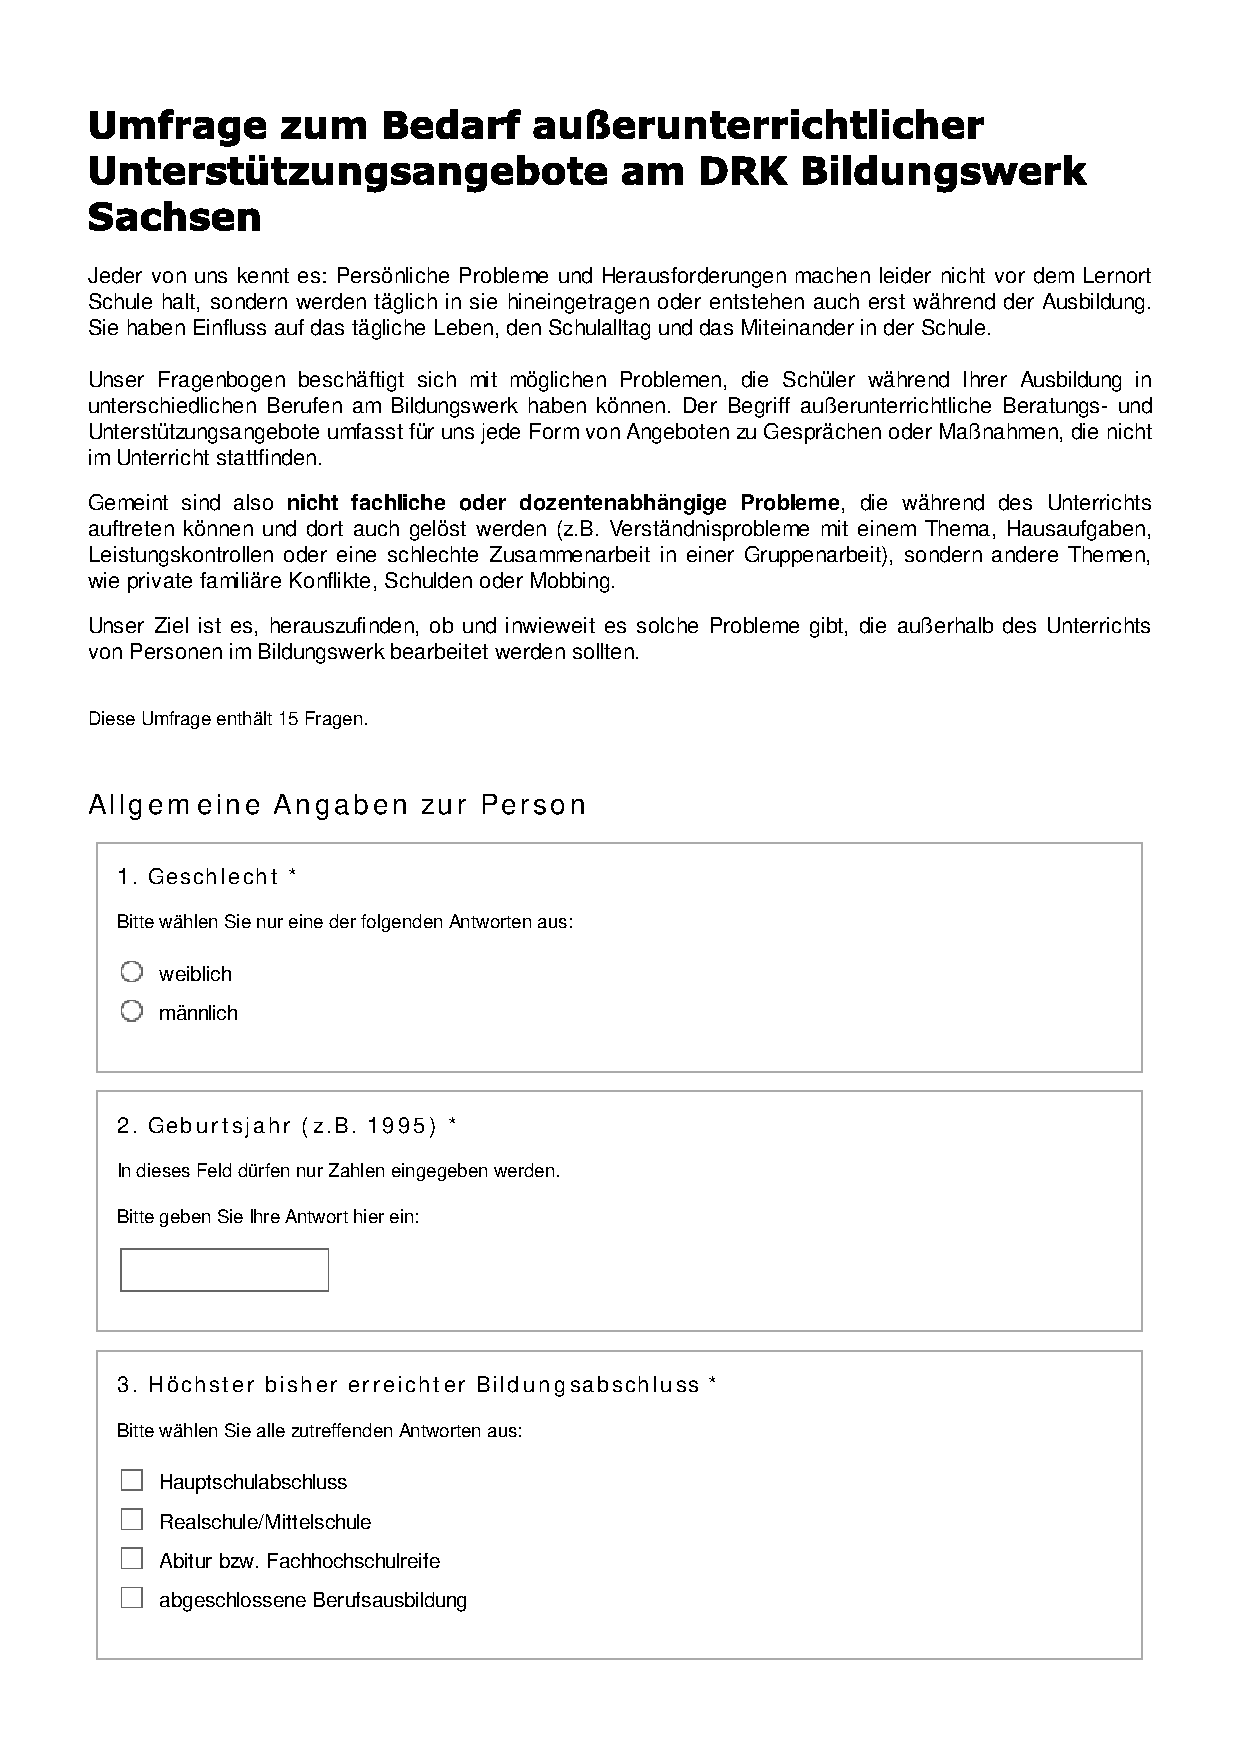
\includepdf[pages=-]{attachments/LimeSurvey-Umfrage-zum-Bedarf-ausserunterrichtlicher-Unterstuetzungsangebote-am-DRK-Bildungswerk-Sachsen.pdf}
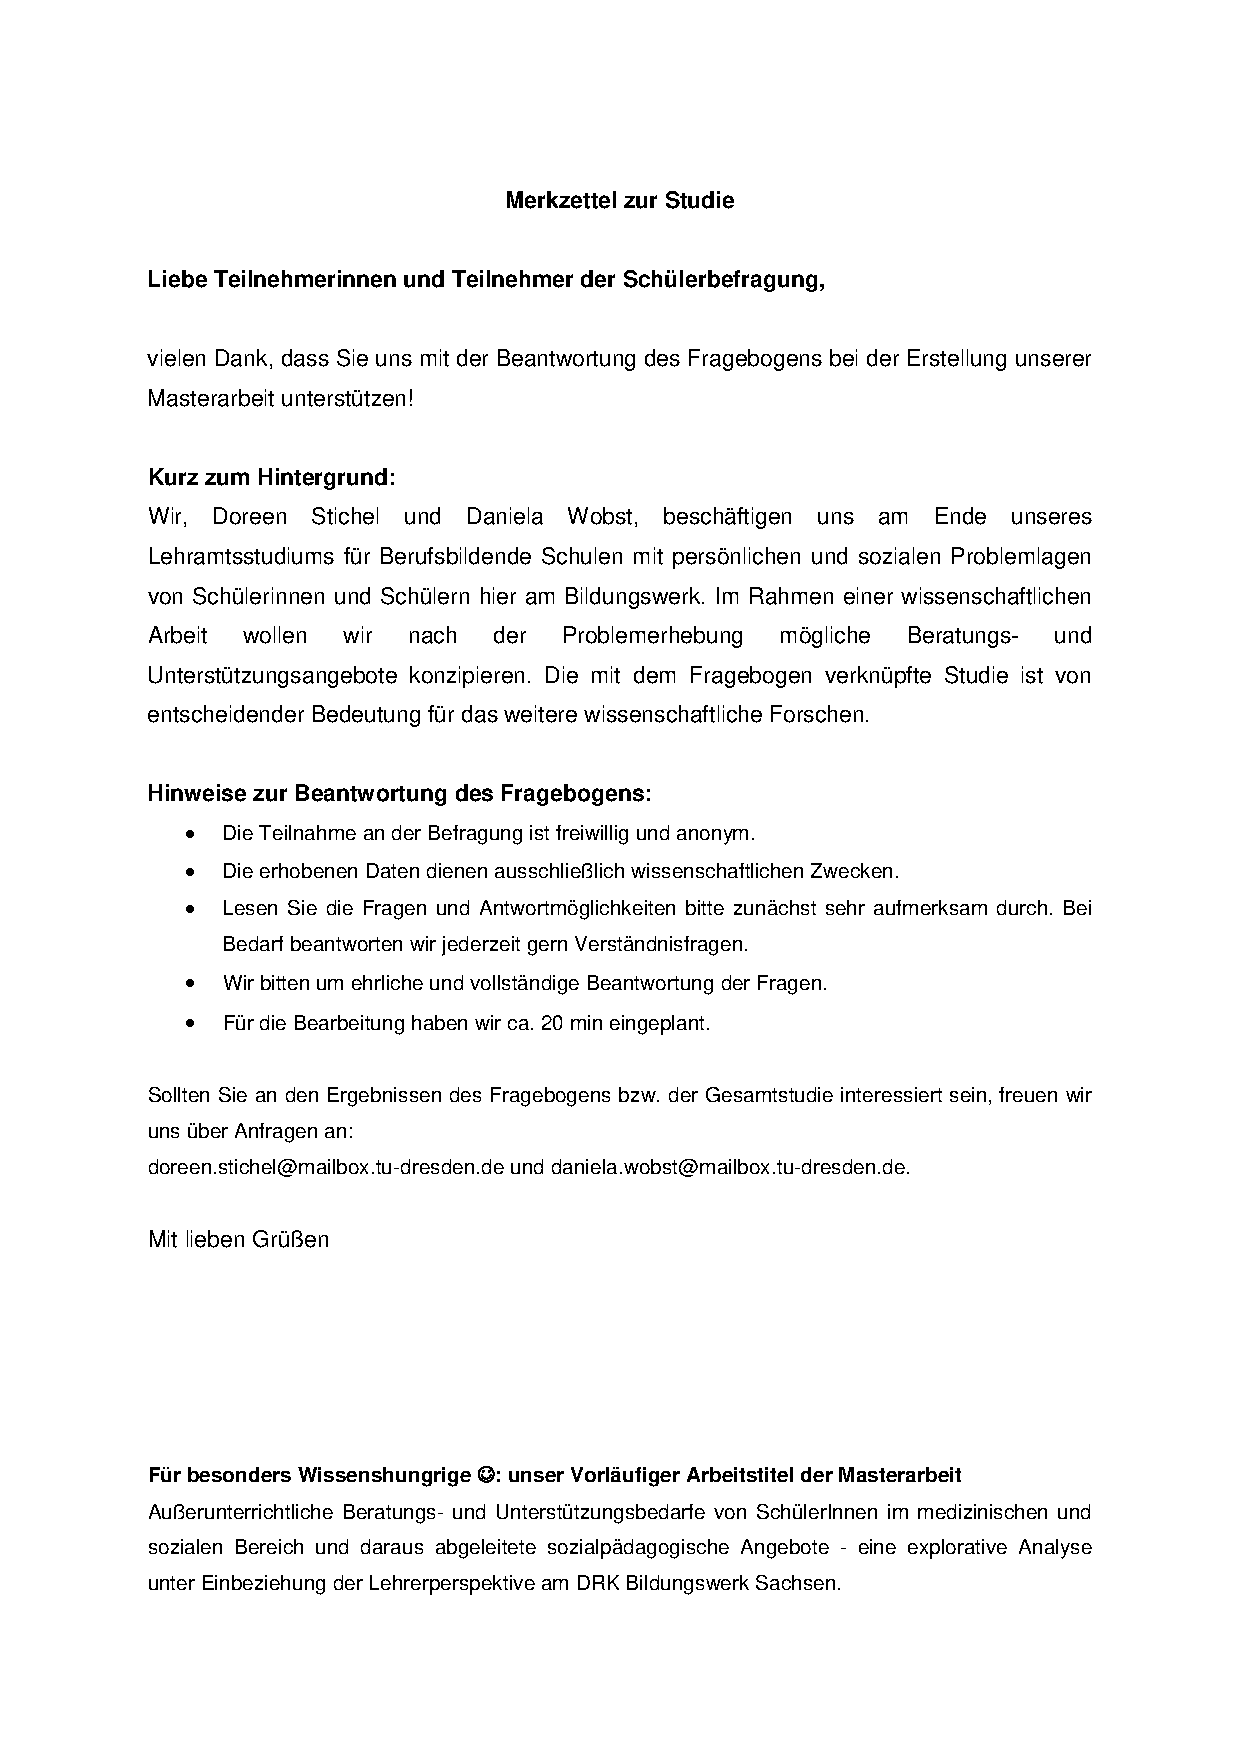
\includepdf[pages=-]{attachments/Merkzettel-zur-Studie.pdf}
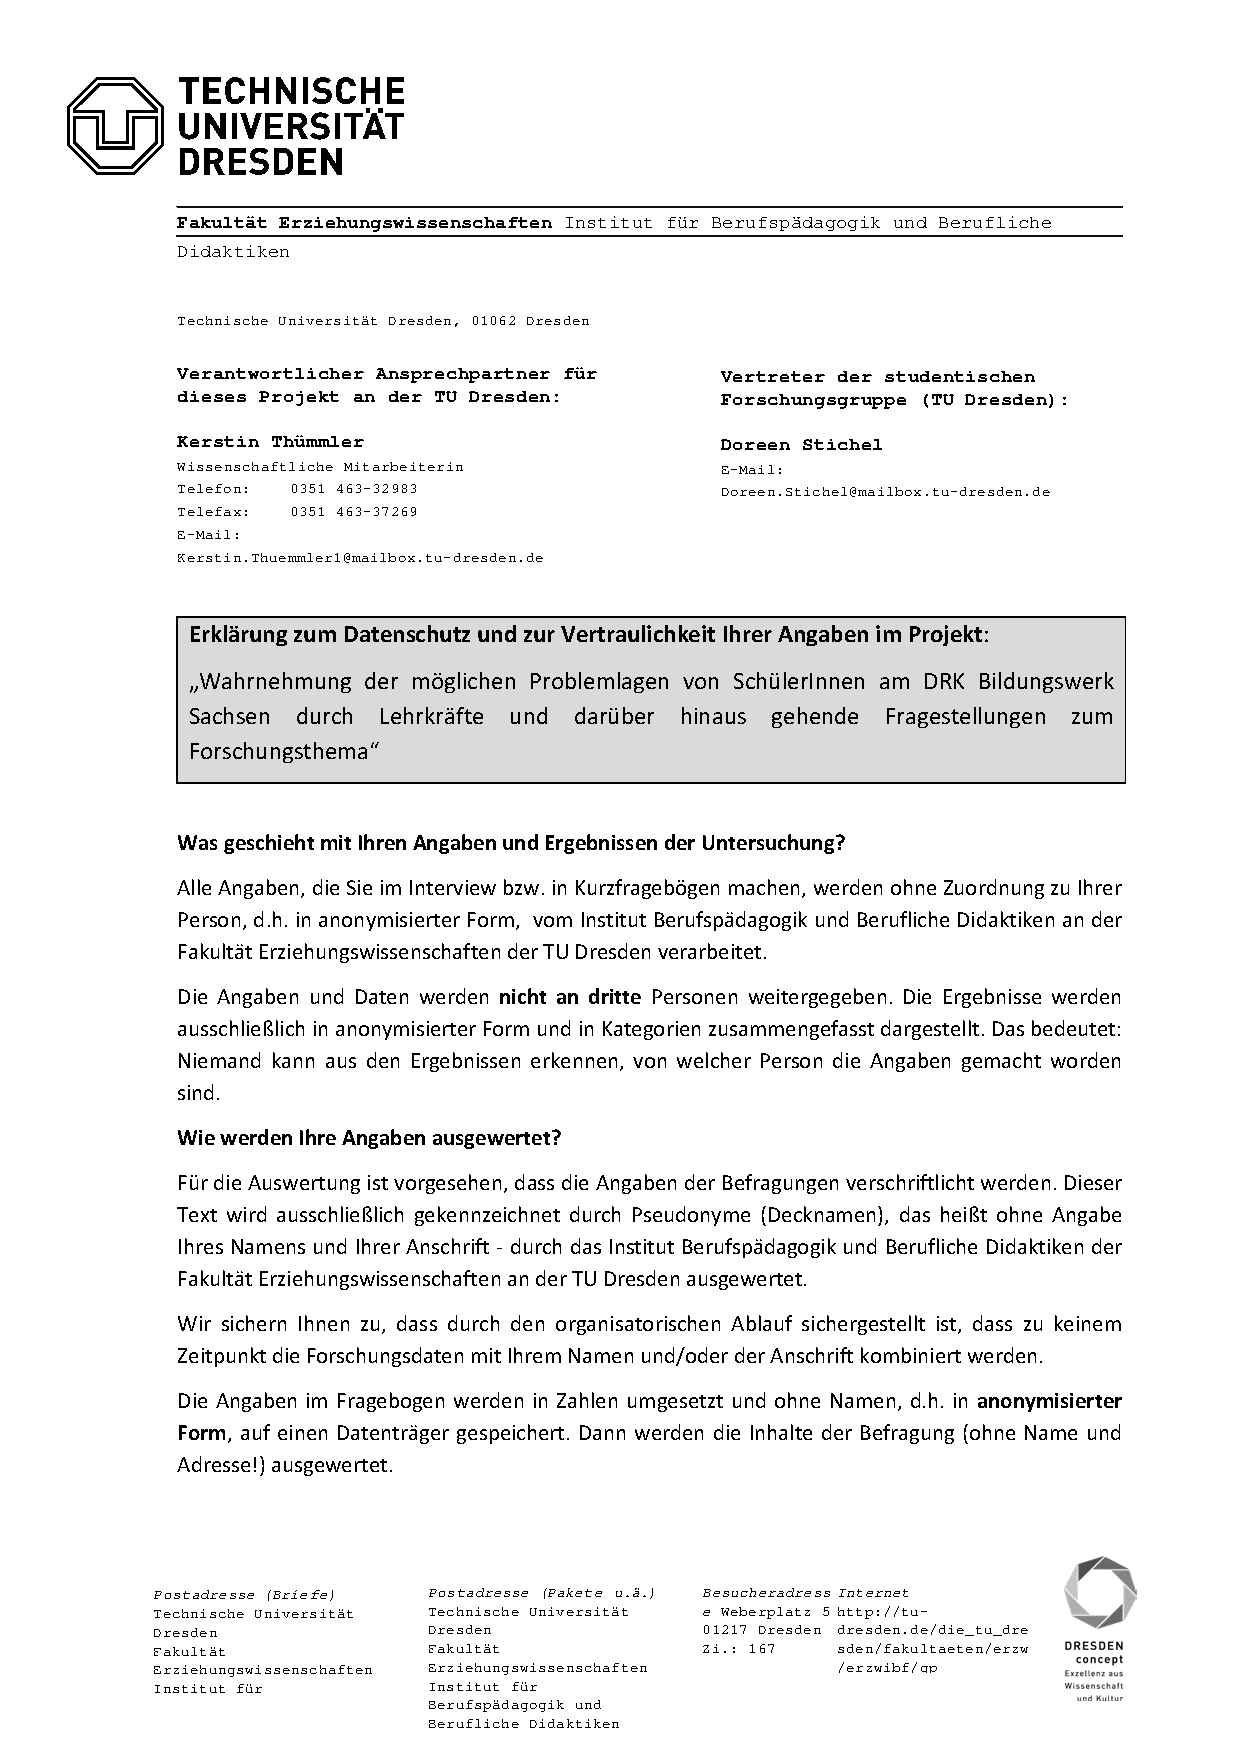
\includepdf[pages=-]{attachments/Datenschutzerklaerung.pdf}

\includepdf[pages=-]{attachments/Einverstaendniserklaerung.pdf}
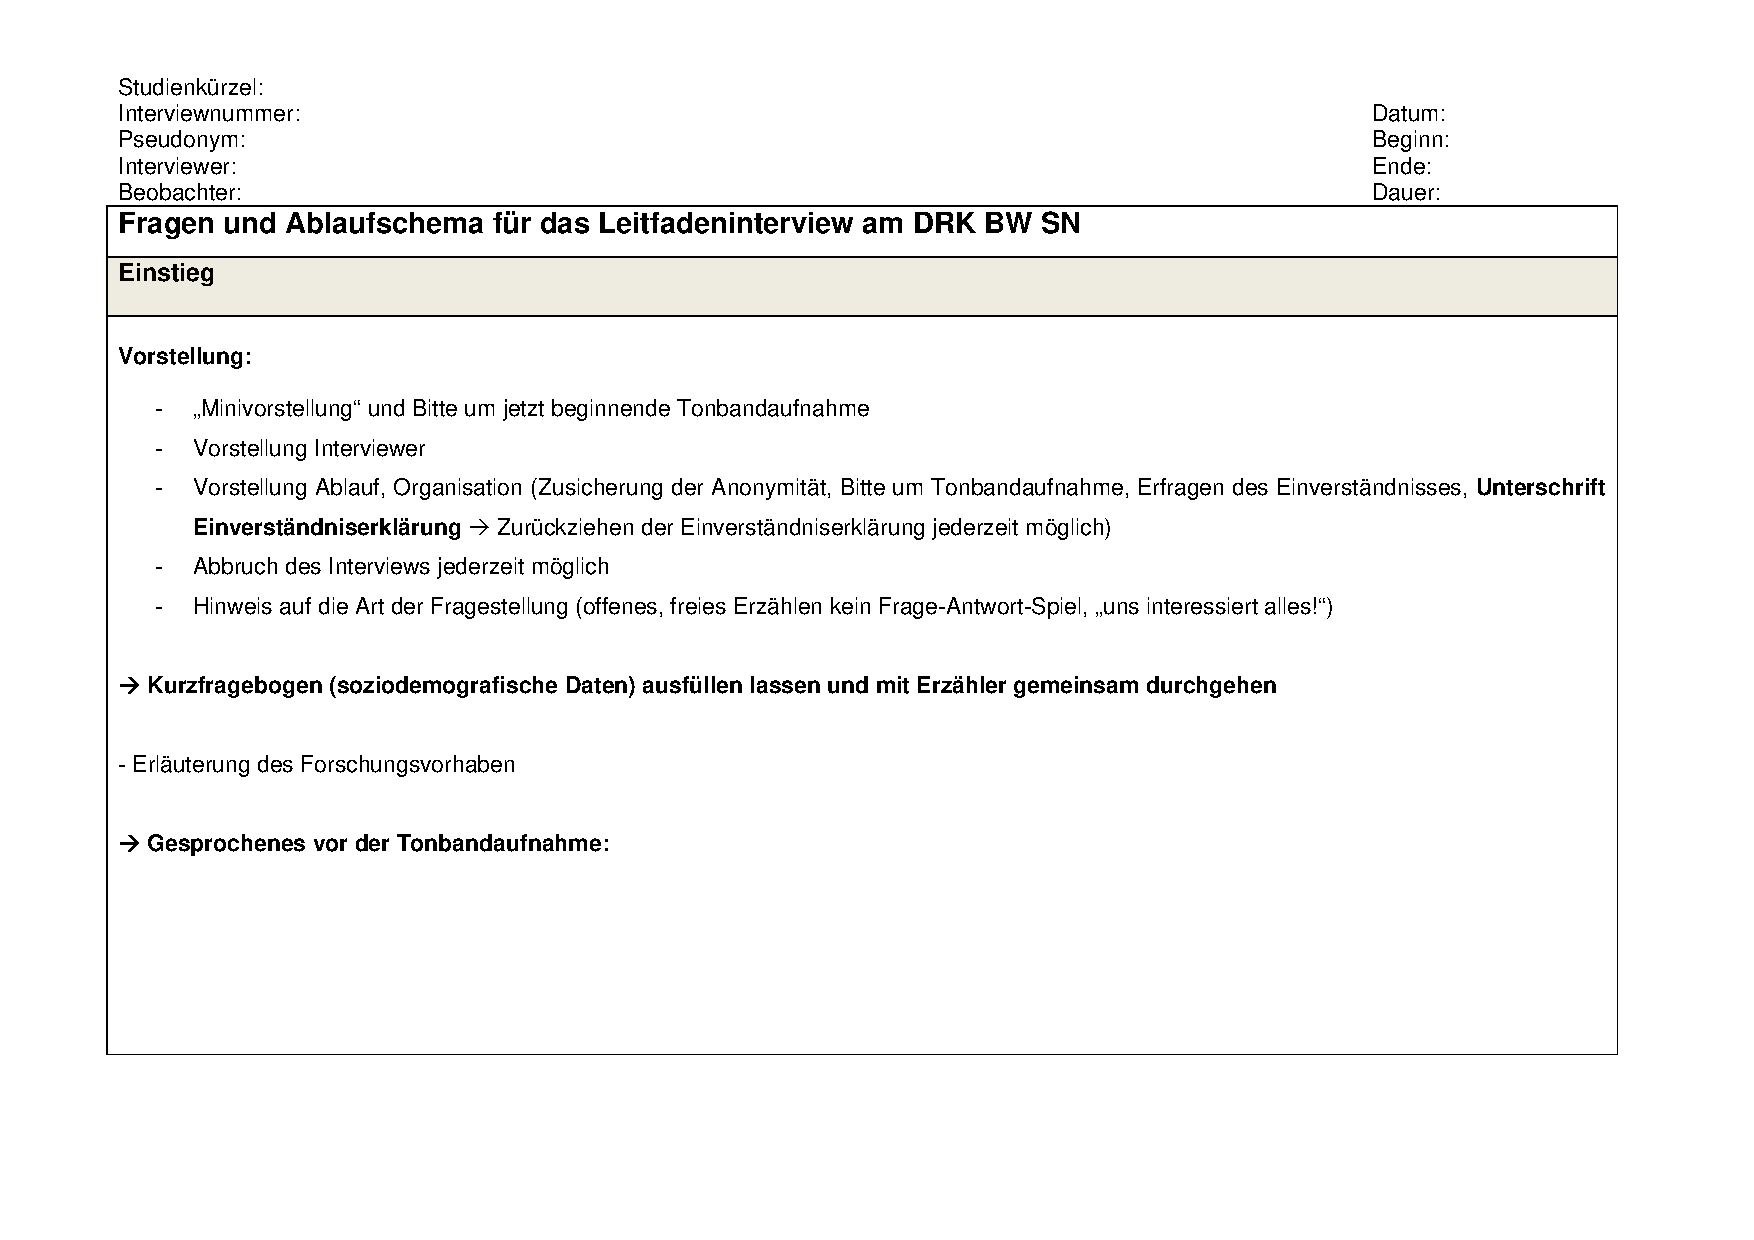
\includepdf[landscape=true,pages=-]{attachments/Struktur-Leitfaden.pdf}
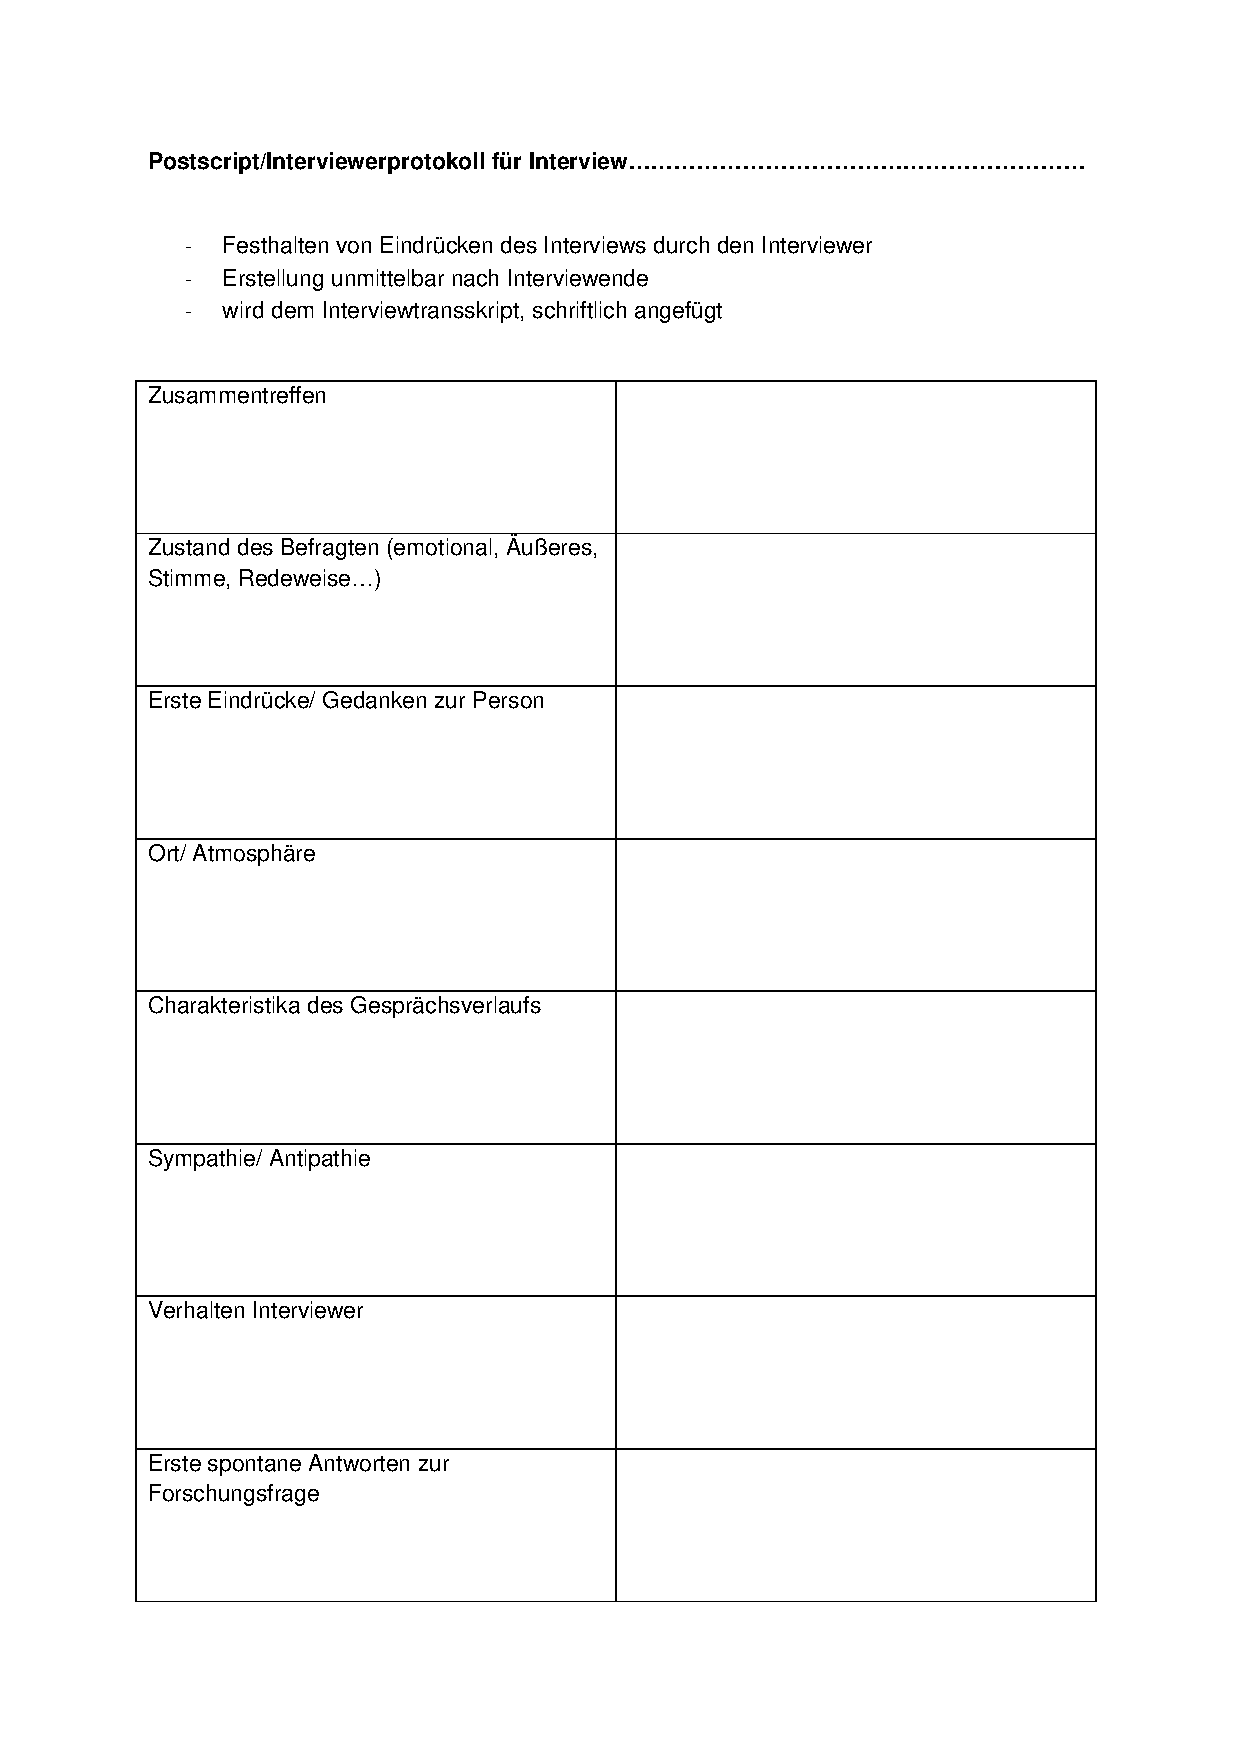
\includepdf[pages=-]{attachments/Postscript.pdf}
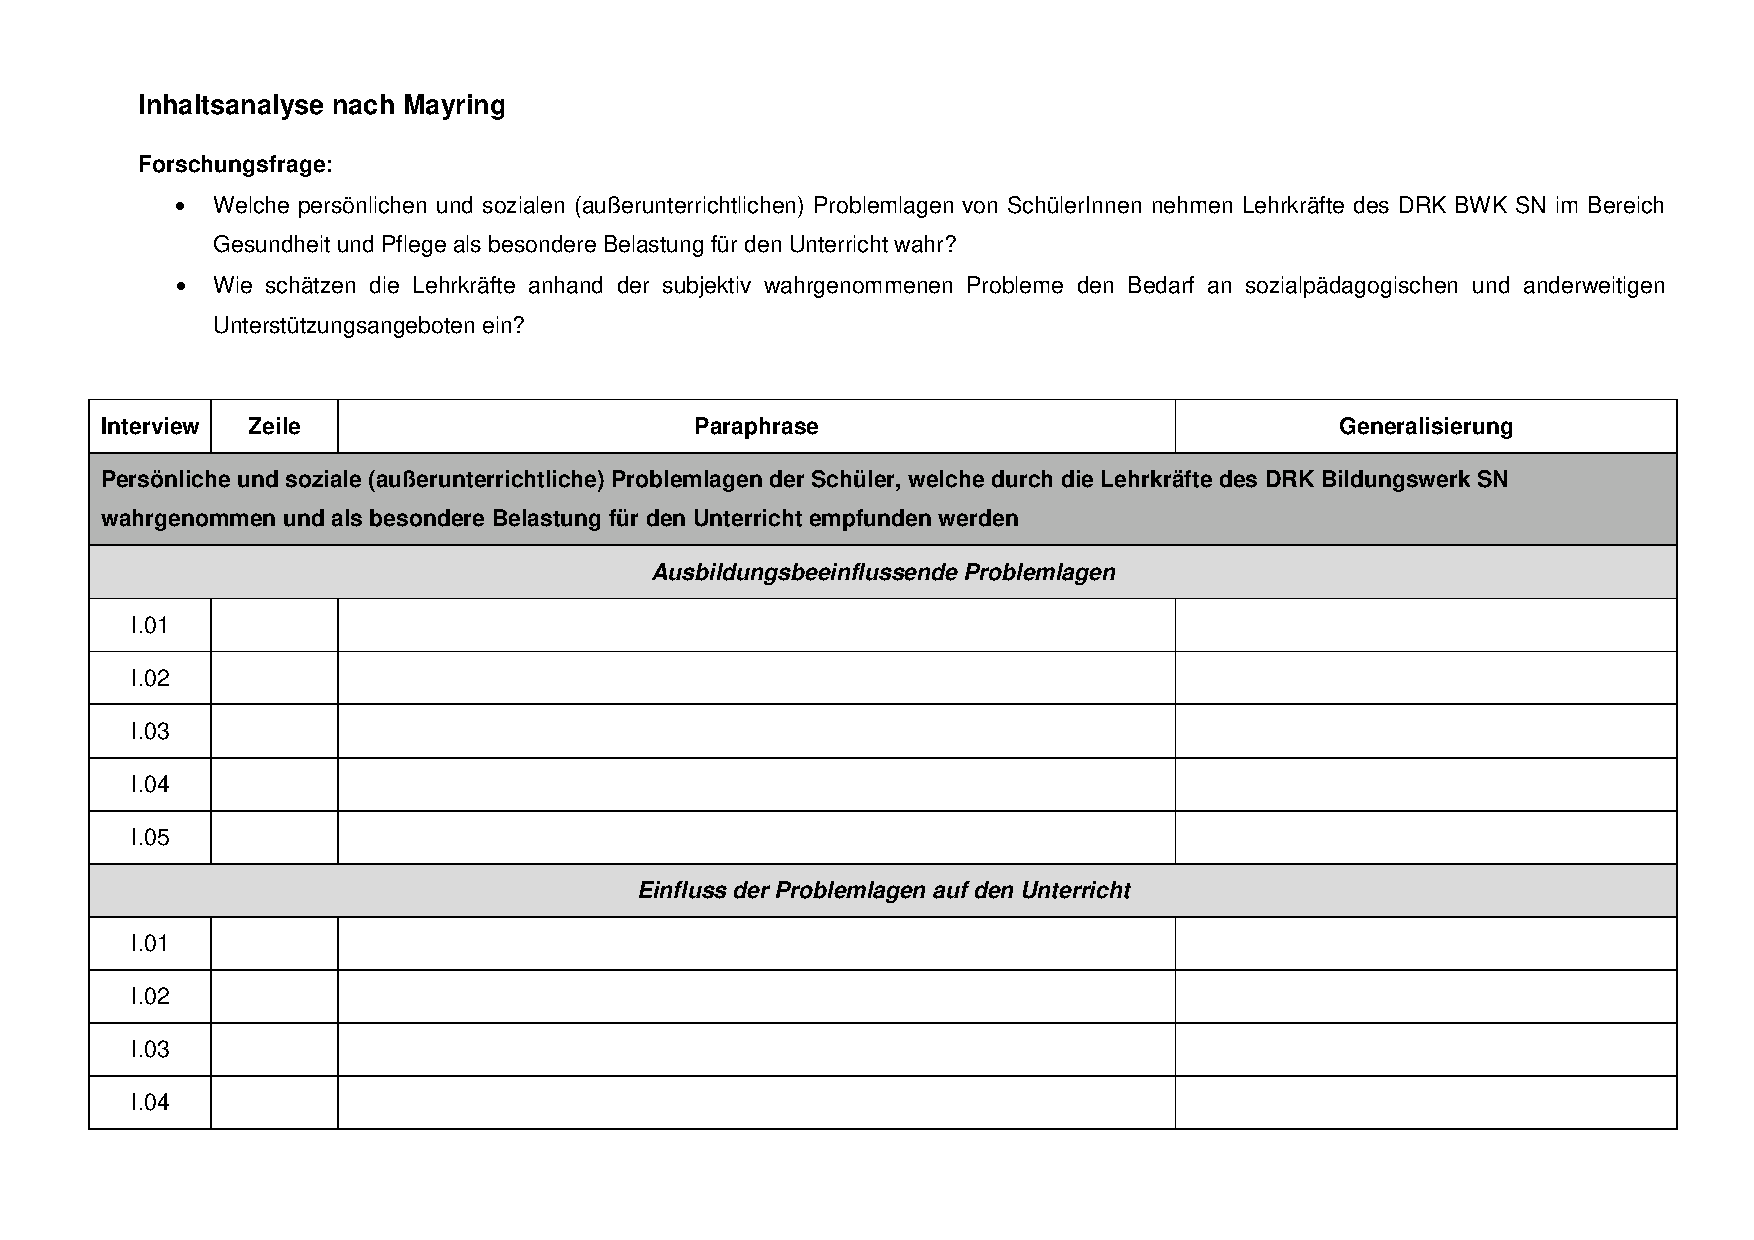
\includepdf[landscape=true,pages=-]{attachments/Vorlage-Paraphrasen-und-Generalisierungen.pdf}
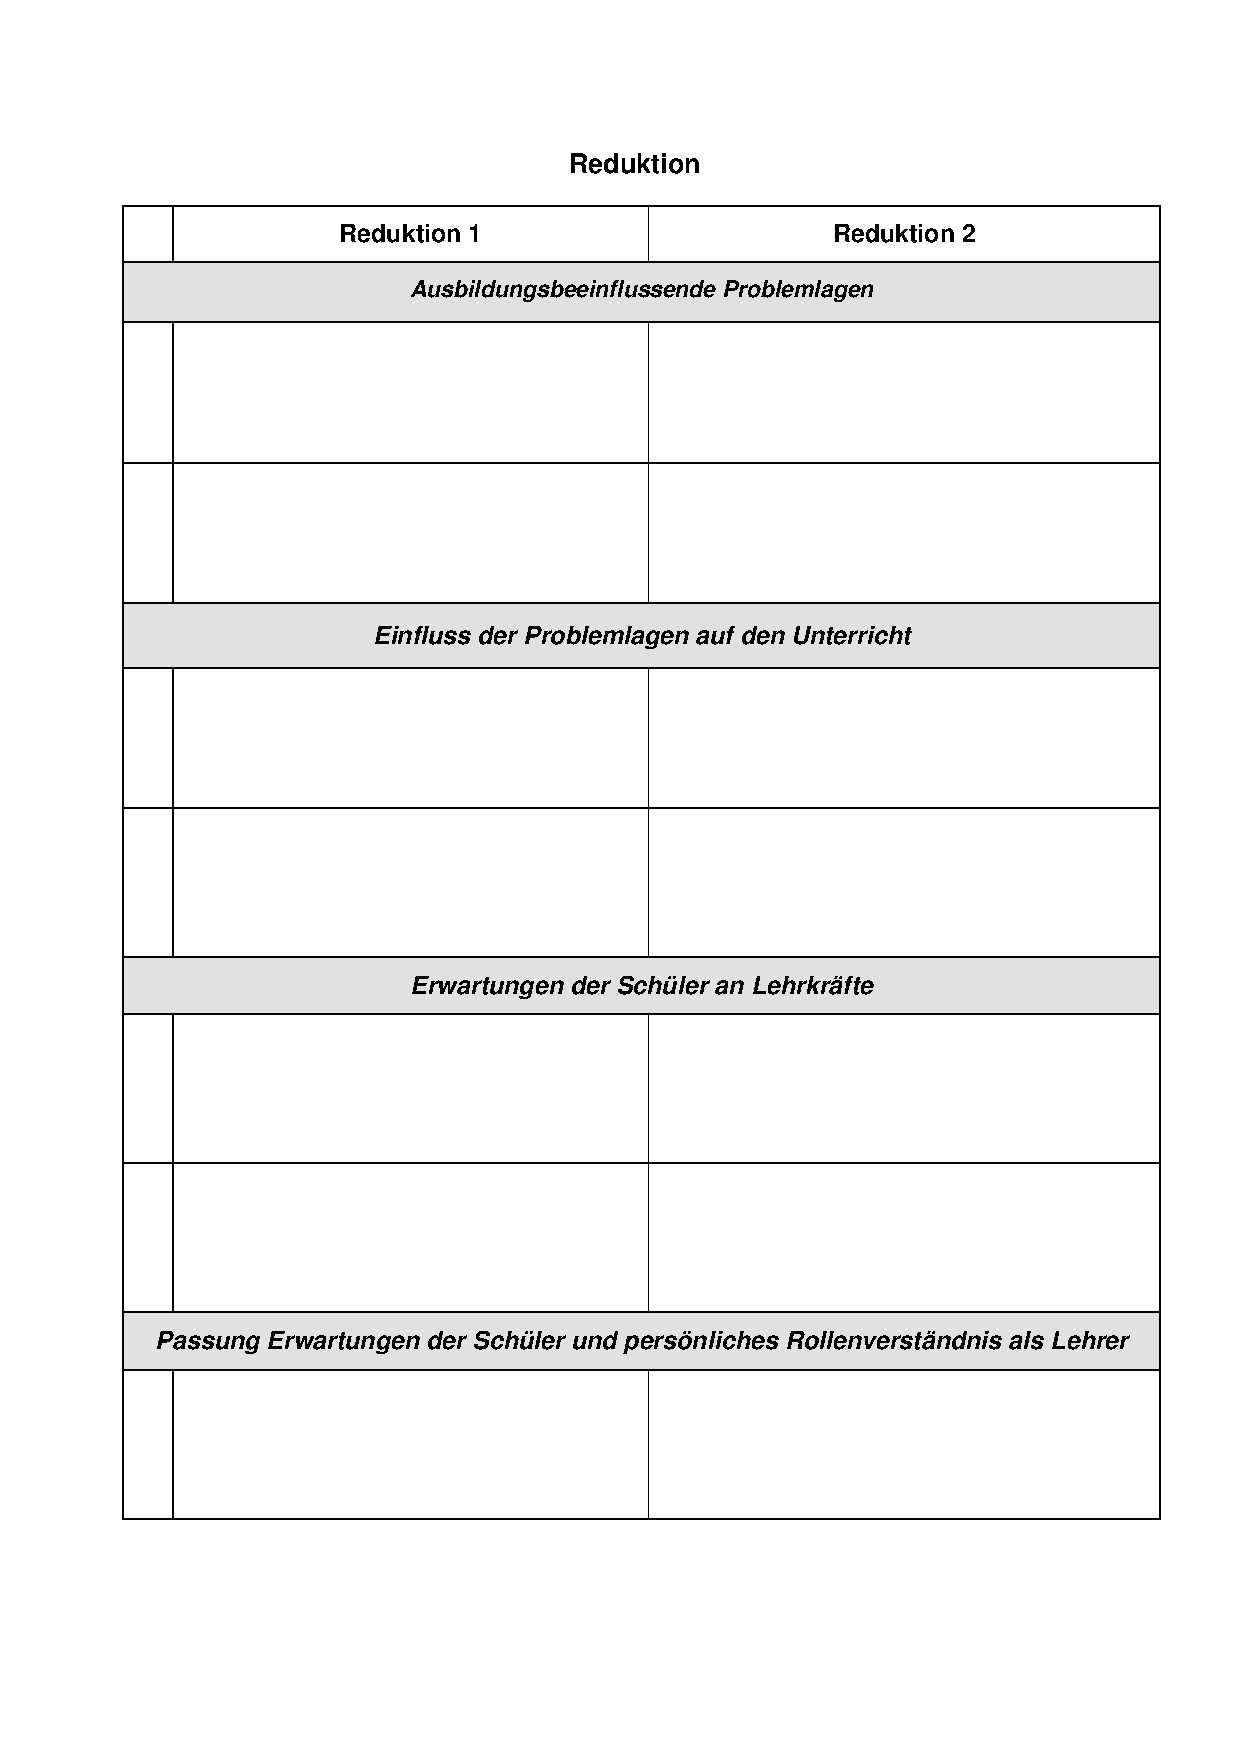
\includepdf[pages=-]{attachments/Vorlage-Reduktion1-und-Reduktion2.pdf}


\listoffigures


%%% Selbstständigkeitserklärung
\section{Selbstständigkeitserklärung}
\label{sec:Selbstständigkeitserklärung}

Ich versichere hiermit, dass ich meinen Anteil an der Arbeit selbstständig verfasst und keine anderen als die angegebenen Quellen und Hilfsmittel benutzt habe.\\[2cm]

$\overline{Stichel, Doreen\hphantom{spaces}\hphantom{spaces}}$ \hfill $\overline{Unterschrift\hphantom{spaces}\hphantom{spaces}}$\\[1cm]

$\overline{Wobst, Daniela\hphantom{spaces}\hphantom{spaces}}$ \hfill $\overline{Unterschrift\hphantom{spaces}\hphantom{spaces}}$\\[2cm]

Dresden, \today

\end{document}
